\documentclass[11pt]{article}

\usepackage[margin=1in]{geometry}
\usepackage{amsmath,amssymb}
\usepackage{bm}
\usepackage{booktabs}
\usepackage{enumitem}
\usepackage{algorithm}
\usepackage{algpseudocode}
\usepackage[numbers,sort&compress]{natbib}
\usepackage{xcolor}
\usepackage{tikz}
\usepackage{graphicx}
\usepackage{caption}
\usepackage[hidelinks]{hyperref}
\usetikzlibrary{arrows.meta,positioning,decorations.pathreplacing,calc}
\emergencystretch=1em
\captionsetup{font=small,labelfont=bf}

\definecolor{tealeafNavy}{HTML}{17324D}
\definecolor{tealeafTeal}{HTML}{168C8C}
\definecolor{tealeafLightTeal}{HTML}{DDF1EF}
\definecolor{tealeafOrange}{HTML}{E6813B}
\definecolor{tealeafLight}{HTML}{F3F6F7}
\definecolor{primerDT}{HTML}{2C7FB8}
\definecolor{primerHex}{HTML}{D95F0E}

\newcommand{\expit}{\operatorname{expit}}
\newcommand{\logit}{\operatorname{logit}}
\newcommand{\BetaDist}{\operatorname{Beta}}
\newcommand{\panel}[1]{\makebox[0pt][l]{\raisebox{-1ex}{\textbf{\sffamily #1}}}}

\title{Differential splicing between cell types from split-pool single-cell RNA-seq with random-hexamer priming}
\author{}
\date{}

\begin{document}
\maketitle

\begin{abstract}
Combinatorial-indexing single-cell RNA-seq profiles hundreds of thousands of cells from tens of donors in one experiment, and its in-cell reverse transcription with random hexamers alongside poly(dT) covers transcript bodies, so the splice junctions of most expressed genes are observed in every cell type of every donor. Methods for differential splicing were designed for bulk or full-length data and use junction-spanning reads of pseudobulk samples. We present Tealeaf, which tests local splice paths, the exon chains that transcripts take through a region bounded by constitutive exons. Every molecule that overlaps the region enters through the set of paths it is compatible with, poly(dT) and random-hexamer molecules enter one likelihood with a label-free primer offset, unannotated paths are built from junction support counted over all cells, and a Beta--logit-normal model with a donor random effect treats donors as replicates. On a mouse brain dataset of 48 animals, Tealeaf replicates more genes across independent halves of the animals than LeafCutter, MAJIQ, scQuint, rMATS and two forms of SUPPA2, its 100 top-ranked tests agree in direction with single-cell long reads as often as the best comparator's, and it has four to twenty-five times as many long-read-evaluable tests. A coverage-only null, applied to every method, shows that MAJIQ and rMATS call many tests from expression differences between cell types alone. In three human blood datasets the top-ranked tests agree with single-cell long reads of a Parse library, and tests between groups of different donors are calibrated.
\end{abstract}

\section{Introduction}

Alternative splicing differs between tissues and cell types \cite{wang2008}, most of all in the nervous system \cite{raj2015}, and single-cell RNA-seq can in principle measure it in every cell type of a tissue at once \cite{arzalluzluque2018}. Droplet methods read the 3$'$ or 5$'$ end of each transcript \cite{zheng2017}, so they observe few splice junctions. Plate methods read whole transcripts \cite{picelli2013,hagemannjensen2020} but profile few cells and donors.

Combinatorial-indexing methods barcode cells in successive rounds of split-pool reactions \cite{cao2017,rosenberg2018,cao2019,martin2023}, so one experiment profiles hundreds of thousands of cells or nuclei from tens of samples, each sample in its own first-round wells. In SPLiT-seq and its commercial form (Parse Biosciences), the first round is reverse transcription inside the cell with a mixture of barcoded poly(dT) and random-hexamer primers \cite{rosenberg2018}, and EasySci combines the two primers in the same way \cite{sziraki2023}. Random-hexamer priming starts along the whole transcript, and the primer of every read is known from its barcode. These data therefore observe splice junctions across transcript bodies, in many cell types and in many donors, the design needed to test splicing differences with donors as biological replicates. In the mouse brain data analysed here, random-hexamer molecules are 45\% of the molecules that overlap alternatively spliced regions and 61\% of those that span a junction distinguishing the alternatives.

Methods for differential splicing were not designed for these data. Event methods (SUPPA2 \cite{trincado2018}, rMATS \cite{shen2014}) test predefined event types, and junction methods (LeafCutter \cite{li2018}, MAJIQ \cite{vaquerogarcia2016,vaquerogarcia2023}, scQuint \cite{benegas2022}) test the relative use of junctions that share a splice site or an exon, from junction-spanning reads of pseudobulk samples. Single-cell methods model cells rather than donors \cite{huang2021,buenabadnajar2022}, and treating cells as replicates inflates false discoveries \cite{squair2021,zimmerman2021}. None uses the reads inside exon bodies, which are most of the reads in a short-read library, and none models the two primers, which sample transcripts with different positional bias.

We present Tealeaf (Testing Exon Alternatives Locally in Exon-Anchored Frames), which tests whether the usage of local splice paths differs between two cell types measured in the same donors, or between two groups of donors within a cell type. We evaluate Tealeaf against six comparators by replication across independent halves of the donors and by agreement of direction with independent single-cell long-read data, after removing, for every method, the tests that a coverage-only null also calls.

\section{Results}

\subsection{Overview of Tealeaf}

Tealeaf works from paired FASTQ files to tests (Fig.~\ref{fig:overview}; Supplementary Fig.~\ref{fig:pipeline}). Reads are aligned to the loci of the target genes by a two-pass spliced aligner that reproduces the scoring and filters of STAR \cite{dobin2013} and replaces whole-genome search for competing alignments by a genome-wide 23-mer uniqueness table (Methods). Against STARsolo \cite{kaminow2021} it reports 97.6\% of STAR's unique alignments in the target loci, with identical junctions for 99.5\% of reads aligned by both, and molecule counts per block, class, donor, cell type and primer agree to within 5\%. A run of 345 million read pairs aligns to all 33{,}755 multi-exon genes in 32 to 67 minutes, against 67 minutes for STARsolo over the whole genome, and its stored alignments take about 1~GB instead of a 46~GB BAM file.

The unit of test is a \emph{splice block}, a window of one gene bounded by constitutive exons in which transcripts take two or more exon chains, the \emph{paths} (Fig.~\ref{fig:overview}b). A path set represents any local pattern, including several adjacent alternative exons, mutually exclusive exons, combinations of alternative splice sites and alternative first or last exons, in one test. Annotated blocks give the annotated paths, and unannotated junctions, with read support counted over all cells and therefore blind to cell-type labels, add novel paths (alternative splice sites, new exons and novel first and last exons) and new blocks (Supplementary Fig.~\ref{fig:novel}). In the brain data the block set has 34{,}677 blocks, 11{,}779 of them new, with 21{,}509 novel paths.

Each UMI molecule that overlaps a block is assigned the set of paths it is compatible with, its \emph{class}, from the parts of its reads inside the block window. A read inside an alternative exon is compatible with the paths that include the exon, and a read inside a constitutive exon with all paths (Fig.~\ref{fig:overview}b). For every path and class, the number of read start positions on the path that produce the class, the \emph{read opportunities}, gives the class probabilities as a function of path usage, so exon-body and junction reads enter one likelihood in proportion to the information they carry. Blocks whose paths differ at a transcript end, \emph{terminal} blocks, use only molecules that span a junction distinguishing the paths, because their exon-body coverage follows the positional capture of the primers (Fig.~\ref{fig:overview}a).

A test compares one block between two cell types (Fig.~\ref{fig:overview}c). Each path is tested against the others with a Beta--logit-normal model in which every donor--cell-type row has its own usage, rows vary around a mean that depends on the cell type through a donor random intercept, and poly(dT) and random-hexamer molecules of a row share the row's usage up to a primer offset estimated without cell-type labels. A likelihood-ratio test of the cell-type effect gives one p-value per path, and the path p-values are combined by Simes' method \cite{simes1986}. Because the donor intercept is shared by the donor's two cell types, the test is paired. The same model compares groups of different donors within a cell type, each donor contributing one row. In count simulations under the null on the real designs, internal tests reject at most 2.9\% of converged fits at nominal 0.05 and at most 1.0\% at 0.01, and junction-only terminal tests 2.7 to 4.3\% at 0.05.

\begin{figure}[t]
\centering
\begin{minipage}[t]{0.47\textwidth}\vspace{0pt}\raggedright\panel{a}\\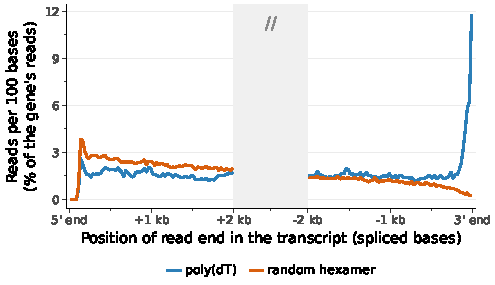
\includegraphics[width=\textwidth]{figures/paper/fig1_profiles.pdf}\end{minipage}\hfill
\begin{minipage}[t]{0.51\textwidth}\vspace{0pt}\raggedright\panel{b}\\[2pt]
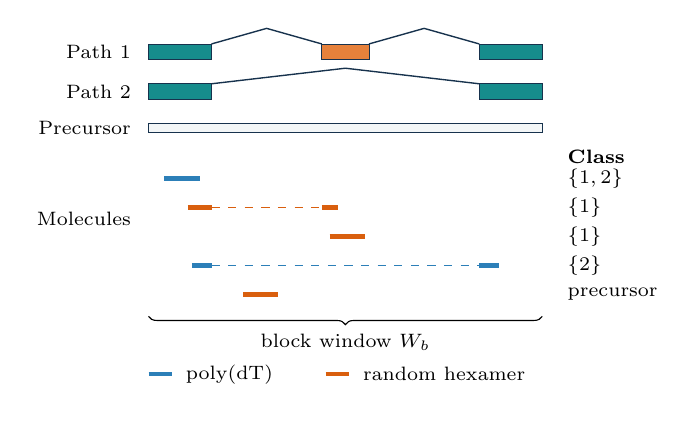
\begin{tikzpicture}[x=0.5mm,y=4.6mm,
  exon/.style={fill=tealeafTeal,draw=tealeafNavy,line width=0.3pt},
  alt/.style={fill=tealeafOrange,draw=tealeafNavy,line width=0.3pt},
  arc/.style={draw=tealeafNavy,line width=0.5pt},
  dT/.style={draw=primerDT,line width=1.6pt},
  hex/.style={draw=primerHex,line width=1.6pt},
  lab/.style={font=\scriptsize,anchor=east},
  cls/.style={font=\scriptsize,anchor=west}]
\node[lab] at (-2,0) {Path 1};
\draw[exon] (0,-0.22) rectangle (16,0.22); \draw[alt] (44,-0.22) rectangle (56,0.22); \draw[exon] (84,-0.22) rectangle (100,0.22);
\draw[arc] (16,0.22) -- (30,0.65) -- (44,0.22); \draw[arc] (56,0.22) -- (70,0.65) -- (84,0.22);
\node[lab] at (-2,-1.1) {Path 2};
\draw[exon] (0,-1.32) rectangle (16,-0.88); \draw[exon] (84,-1.32) rectangle (100,-0.88);
\draw[arc] (16,-0.88) -- (50,-0.45) -- (84,-0.88);
\node[lab] at (-2,-2.1) {Precursor};
\draw[fill=tealeafLight,draw=tealeafNavy,line width=0.3pt] (0,-2.22) rectangle (100,-1.98);
\node[font=\scriptsize\bfseries,anchor=west] at (104,-2.9) {Class};
\node[lab] at (-2,-4.6) {Molecules};
\draw[dT] (4,-3.5) -- (13,-3.5); \node[cls] at (104,-3.5) {$\{1,2\}$};
\draw[hex] (10,-4.3) -- (16,-4.3); \draw[primerHex,line width=0.4pt,dashed] (16,-4.3) -- (44,-4.3); \draw[hex] (44,-4.3) -- (48,-4.3); \node[cls] at (104,-4.3) {$\{1\}$};
\draw[hex] (46,-5.1) -- (55,-5.1); \node[cls] at (104,-5.1) {$\{1\}$};
\draw[dT] (11,-5.9) -- (16,-5.9); \draw[primerDT,line width=0.4pt,dashed] (16,-5.9) -- (84,-5.9); \draw[dT] (84,-5.9) -- (89,-5.9); \node[cls] at (104,-5.9) {$\{2\}$};
\draw[hex] (24,-6.7) -- (33,-6.7); \node[cls] at (104,-6.7) {precursor};
\draw[decorate,decoration={brace,mirror,amplitude=3pt}] (0,-7.3) -- (100,-7.3) node[midway,below=3pt,font=\scriptsize] {block window $W_b$};
\draw[primerDT,line width=1.6pt] (0,-8.9) -- (6,-8.9); \node[cls] at (7,-8.9) {poly(dT)};
\draw[primerHex,line width=1.6pt] (45,-8.9) -- (51,-8.9); \node[cls] at (52,-8.9) {random hexamer};
\end{tikzpicture}

\end{minipage}\\[6pt]
\begin{minipage}[t]{\textwidth}\raggedright\panel{c}\\[2pt]\centering
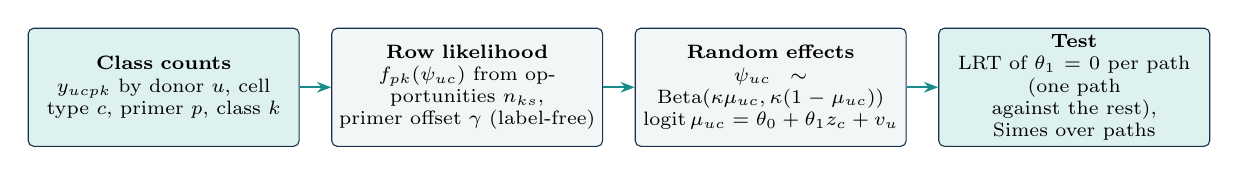
\begin{tikzpicture}[
  box/.style={draw=tealeafNavy,rounded corners=2pt,fill=tealeafLight,align=center,font=\scriptsize,text width=33mm,minimum height=15mm,inner sep=2pt},
  flow/.style={-{Stealth[length=1.8mm]},thick,draw=tealeafTeal},
  node distance=4mm]
\node[box,fill=tealeafLightTeal] (counts) {\textbf{Class counts}\\$y_{ucpk}$ by donor $u$, cell type $c$, primer $p$, class $k$};
\node[box,right=of counts] (row) {\textbf{Row likelihood}\\$f_{pk}(\psi_{uc})$ from opportunities $n_{ks}$,\\primer offset $\gamma$ (label-free)};
\node[box,right=of row] (model) {\textbf{Random effects}\\$\psi_{uc}\sim\BetaDist(\kappa\mu_{uc},\kappa(1-\mu_{uc}))$\\$\logit\mu_{uc}=\theta_0+\theta_1z_c+v_u$};
\node[box,right=of model,fill=tealeafLightTeal] (test) {\textbf{Test}\\LRT of $\theta_1=0$ per path\\(one path against the rest),\\Simes over paths};
\draw[flow] (counts)--(row); \draw[flow] (row)--(model); \draw[flow] (model)--(test);
\end{tikzpicture}

\end{minipage}
\caption{Tealeaf. \textbf{a}, Density of read ends by spliced distance from the 5$'$ and 3$'$ ends of 1{,}500 to 1{,}700 long single-isoform genes per library, relative to the density in the transcript middle, for poly(dT) and random-hexamer molecules of the brain data. \textbf{b}, A splice block with an alternative exon between two constitutive anchor exons, its two paths and the precursor (the unspliced window), and molecules of each class. A molecule's class is the set of paths compatible with its reads inside the window; the read opportunities $n_{ks}$ count the read start positions on path $s$ that give class $k$. \textbf{c}, The test. Class counts of each donor $u$, cell type $c$ and primer $p$ follow from the row usage $\psi_{uc}$ through the opportunities, with a primer offset $\gamma$; $\psi_{uc}$ varies around a mean with a cell-type effect $\theta_1$ and a donor intercept $v_u$, each path is tested against the others by a likelihood-ratio test of $\theta_1=0$, and the path p-values are combined by Simes' method.}
\label{fig:overview}
\end{figure}

\subsection{Evaluation design}

We evaluated Tealeaf on a Parse dataset of mouse brain nuclei from 48 animals in six groups of eight (wild type, the microglia-deficient FIRE line \cite{rojo2019}, 5xFAD \cite{oakley2006}, 5xFAD crossed to FIRE \cite{kianishabestari2022}, and the cross treated with PBS or with a microglia transplant), with 37{,}002 nuclei in 19 cell types and 5.6 billion read pairs. Every pair of cell types is tested.

Two endpoints are used, neither of which needs knowledge of the true splicing differences. For \emph{split replication}, the animals are divided into two halves of 24, balanced by group, and each method is run on each half. A gene replicates when it has signal in both halves, by the BH-adjusted \cite{benjamini1995} conjunction of its two half p-values, each the Simes combination over the gene's tests. Each comparison is scored on the comparator's own universe of (gene, cell-type pair) keys tested in both halves, and on the matched universe, its intersection with the keys Tealeaf tests. For \emph{long-read direction}, the effects of full-data tests are compared with the P56 mouse brain single-cell long-read data of Joglekar et al.\ \cite{joglekar2024}, in eight cell types with a prespecified correspondence. Long-read transcripts are assigned to the tested paths (or junctions or events) of every method by their exon chains in the comprehensive annotation, and the endpoint is the normalized area $A_{100}$ under the cumulative agreement of the 100 top-ranked evaluable tests, ranked by p-value. Split replication does not use direction, and long-read direction does not use replication.

The comparators are LeafCutter, MAJIQ Heterogen, scQuint, paired rMATS (PAIRADISE \cite{demirdjian2020}), SUPPA2 with exact paired signed-rank tests on donor pseudobulks, and a primer-aware SUPPA2 that estimates event usage from the Tealeaf molecule classes with a primer offset (Methods). Each is run on the same donor--cell-type pseudobulks, cell-type pairs and halves. For every method, tests that a coverage-only null also calls are removed before both endpoints (Methods). In this null each sample keeps its coverage of the tested feature and the two cell types share one usage, so a test it calls is driven by coverage, not by splicing. Among the tests that each method's null recomputes ($p<0.01$ on the data), the filter removes 0 to 0.9\% for Tealeaf, LeafCutter and scQuint, close to the 0.7\% expected by chance, 8 to 12\% for rMATS and 43 to 68\% for MAJIQ (Supplementary Table~\ref{tab:coverage-removed}). SUPPA2 is not recomputed.

\subsection{Tealeaf replicates more genes in mouse brain}

On each comparator's matched universe Tealeaf replicates more genes than the comparator (Fig.~\ref{fig:brain}a): 63 against 35 for LeafCutter, 201 against 17 for MAJIQ, 179 against 134 for scQuint, 158 against 4 for rMATS, 124 against 8 for SUPPA2 and 130 against 0 for primer-aware SUPPA2. The comparator universes give the same order (Supplementary Table~\ref{tab:results}). The matched universes differ in size from 263 genes for LeafCutter to 5{,}070 for rMATS, because each method tests the genes where its own features have data in both halves.

Tealeaf's 100 top-ranked long-read-evaluable tests agree with the long reads in direction for 95 ($A_{100}=0.946$), MAJIQ's after the filter for 90 ($0.944$), and those of the other comparators for 77 to 90, except primer-aware SUPPA2 (69; Fig.~\ref{fig:brain}b). Agreement holds further down the ranking. At rank 200 Tealeaf agrees for 94\% of its tests against 80 to 85\% for the junction methods and 81\% for rMATS. Tealeaf has 33{,}872 evaluable tests, against 1{,}351 to 8{,}489 features for the junction methods and 2{,}773 to 4{,}444 events for rMATS and SUPPA2 on their 500 top-ranked events per contrast (Fig.~\ref{fig:brain}c).

On the 28 pairs of the long-read cell types, the contrasts every method tests, Tealeaf makes 3{,}600 discoveries (BH 0.05 within method) in 3{,}005 gene--cell-type pairs, scQuint 2{,}205 pairs, LeafCutter 351, SUPPA2 350, MAJIQ 263, primer-aware SUPPA2 233 and rMATS 164 (Fig.~\ref{fig:brain}d). Tealeaf discovers 1{,}010 cassette exons against 321 for SUPPA2 and 166 for rMATS, and 1{,}464 of its discoveries are alternative first or last exons, which the event sets of SUPPA2 and rMATS do not contain. Over all 190 pairs, Tealeaf has 8{,}975 gene--cell-type pairs with a discovery and scQuint 8{,}742 (Supplementary Fig.~\ref{fig:discoveries-all}). By event class, long-read agreement of Tealeaf's evaluable discoveries is 0.83 to 0.90 for the common classes, and 6{,}895 of its 10{,}742 full-data discoveries retain an unannotated path (Supplementary Table~\ref{tab:events}).

\begin{figure}[t]
\centering
\begin{minipage}[t]{0.5\textwidth}\vspace{0pt}\raggedright\panel{a}\\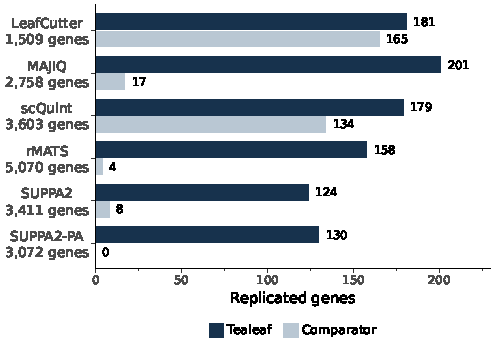
\includegraphics[width=\textwidth]{figures/paper/fig2_split.pdf}\end{minipage}\hfill
\begin{minipage}[t]{0.49\textwidth}\vspace{0pt}\raggedright\panel{b}\\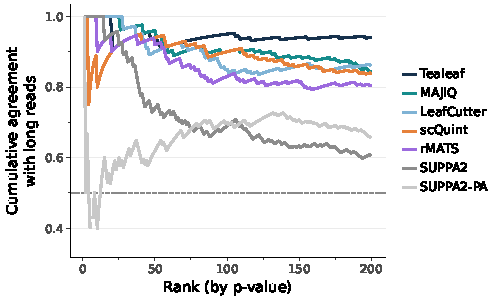
\includegraphics[width=\textwidth]{figures/paper/fig2_lr.pdf}\end{minipage}\\[4pt]
\begin{minipage}[t]{0.37\textwidth}\vspace{0pt}\raggedright\panel{c}\\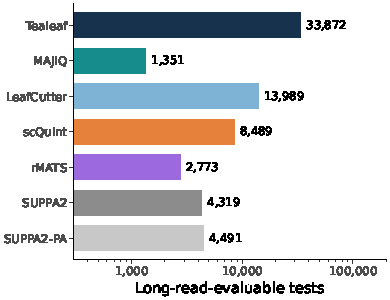
\includegraphics[width=\textwidth]{figures/paper/fig2_evaluable.pdf}\end{minipage}\hfill
\begin{minipage}[t]{0.62\textwidth}\vspace{0pt}\raggedright\panel{d}\\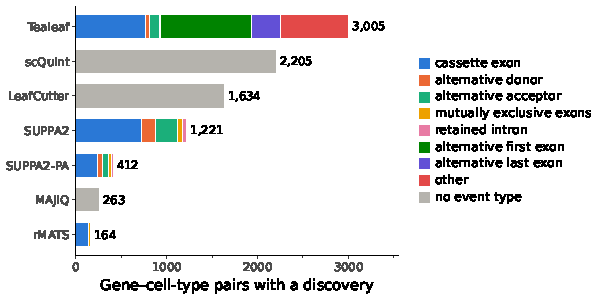
\includegraphics[width=\textwidth]{figures/paper/fig2_discoveries.pdf}\end{minipage}
\caption{Mouse brain. \textbf{a}, Genes replicated across the two halves of the animals by Tealeaf and by each comparator, on the comparator's matched universe (number of genes under the name; SUPPA2-PA is primer-aware SUPPA2). \textbf{b}, Cumulative agreement with long-read directions among the top-ranked full-data tests (Tealeaf) or features (comparators); the dashed line is chance. \textbf{c}, Number of long-read-evaluable tests or features (SUPPA2 and rMATS, 500 top-ranked events per contrast). \textbf{d}, Gene--cell-type pairs with a full-data discovery (BH 0.05 within method) on the 28 pairs of the long-read cell types, by the event class of the pair's smallest-p discovery. LeafCutter, scQuint and MAJIQ test junction clusters, which have no event class. Tests called by the coverage-only null are removed for every method except SUPPA2.}
\label{fig:brain}
\end{figure}

\subsection{Coverage differences produce calls of MAJIQ and rMATS}

Without the coverage-only filter, MAJIQ and rMATS replicate 27 and 4 genes on their matched brain universes, and 991 and 184 on their universes in the human blood dataset GSE320507 described below. To see whether these replications reflect splicing, we recomputed each method's tests on data with the observed coverage and no difference in usage between the cell types. MAJIQ Heterogen compares per-sample PSI estimates whose prior pulls them toward a fixed value at low coverage, so a gene expressed at different levels in two cell types gives significant tests without a difference in PSI (Supplementary Note~\ref{sec:majiq-null}). Under the coverage-only null its call rate follows the coverage ratio between the two cell types and reaches 93\% of tests when the ratio exceeds eightfold, against 94\% on the data (Fig.~\ref{fig:null}a). Because expression differences between cell types are shared by all donors, these calls replicate across halves. In the same null, Tealeaf rejects 0 to 6\% of internal and 2 to 4\% of terminal tests at nominal 0.05 in every class of the coverage ratio, and LeafCutter and scQuint make no discoveries. rMATS, run through PAIRADISE on four whole contrasts of null counts, makes about as many BH calls of mutually exclusive exons as on the data and more of skipped exons (Fig.~\ref{fig:null}c), rejecting 10 to 13\% of skipped-exon and 40 to 51\% of mutually-exclusive-exon tests at 0.05. Most rMATS mutually-exclusive-exon calls in these data have both exons in one annotated transcript, so the event compares junctions of different isoforms.

The filter keeps a test unless the null calls it, so it removes coverage-driven tests but does not recalibrate the remaining ones. It removes 0 to 0.9\% of the recomputed tests of Tealeaf, LeafCutter and scQuint, 8 to 27\% for rMATS and 43 to 96\% for MAJIQ (Fig.~\ref{fig:null}b). After the filter, MAJIQ replicates 17 genes on its matched brain universe and its 100 top-ranked features agree with the long reads for 90; the results without the filter are given in Supplementary Note~\ref{sec:unfiltered}.

\begin{figure}[t]
\centering
\begin{minipage}[t]{0.34\textwidth}\vspace{0pt}\raggedright\panel{a}\\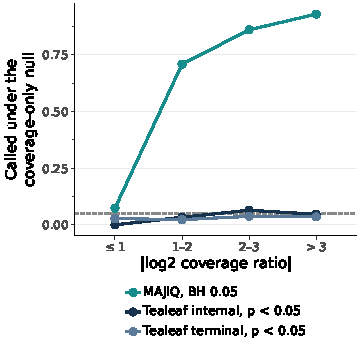
\includegraphics[width=\textwidth]{figures/paper/fig4_null_coverage.pdf}\end{minipage}\hfill
\begin{minipage}[t]{0.33\textwidth}\vspace{0pt}\raggedright\panel{b}\\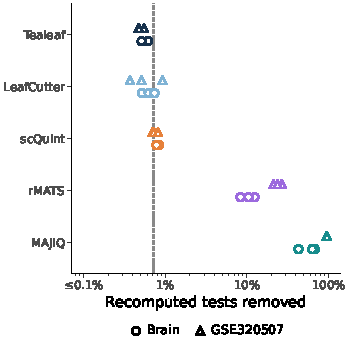
\includegraphics[width=\textwidth]{figures/paper/fig4_removed.pdf}\end{minipage}\hfill
\begin{minipage}[t]{0.31\textwidth}\vspace{0pt}\raggedright\panel{c}\\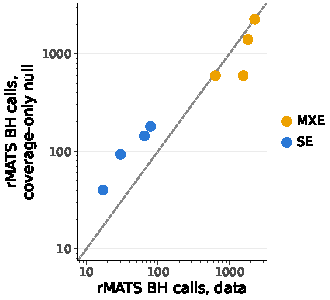
\includegraphics[width=\textwidth]{figures/paper/fig4_rmats.pdf}\end{minipage}
\caption{Coverage-only null. \textbf{a}, Fraction of tests called under the coverage-only null by the absolute log$_2$ ratio of coverage between the two cell types in GSE320507: MAJIQ Heterogen edges at BH 0.05 within contrast, and Tealeaf tests (200 per structure) at nominal $p<0.05$ among converged fits. The dashed line is 0.05. \textbf{b}, Fraction of recomputed tests ($p<0.01$ on the data) that the null calls (median of three null p-values below 0.05) and that are removed, per method and run (full data and the two halves), in brain and GSE320507; the dashed line is the 0.7\% expected for a calibrated test. \textbf{c}, BH calls of paired rMATS on four whole GSE320507 contrasts, on the data and on counts redrawn without a difference in inclusion, for skipped exons (SE) and mutually exclusive exons (MXE).}
\label{fig:null}
\end{figure}

\subsection{Examples in mouse brain}

The full-data tests with the largest effect among those evaluable in the long reads, selected without regard to long-read agreement ($p<10^{-8}$, at least 50 long-read UMIs per cell type, at most four paths, one per gene, at least one internal and one terminal block), all agree with the long reads in direction (Fig.~\ref{fig:examples}; Supplementary Figs.~\ref{fig:nfasc}--\ref{fig:usage}). In \emph{Pkn2}, astrocytes include a cassette exon in 68\% of molecules and cortical excitatory neurons in 27\% (means over 13 animals with both cell types); the long reads show inclusion in 100\% and 87\% of transcripts that span the block. The direction agrees, but cortical neurons skip the exon in 73\% of Parse molecules and 13\% of long-read transcripts. In \emph{Mctp1}, a terminal block with two first exons tens of kilobases apart, dentate gyrus granule neurons use the upstream first exon in 74\% of junction-spanning molecules and medium spiny neurons in 15\% (long-read shares 33\% and 18\%). The other two examples are a short cassette exon in \emph{Nfasc} and a 21-base cassette exon in \emph{Kif21a}, where a second 21-base exon in the same block carries 0.4\% of molecules and is removed by the share screen.

\begin{figure}[p]
\centering
\begin{minipage}{\textwidth}\raggedright\panel{a}\\\centering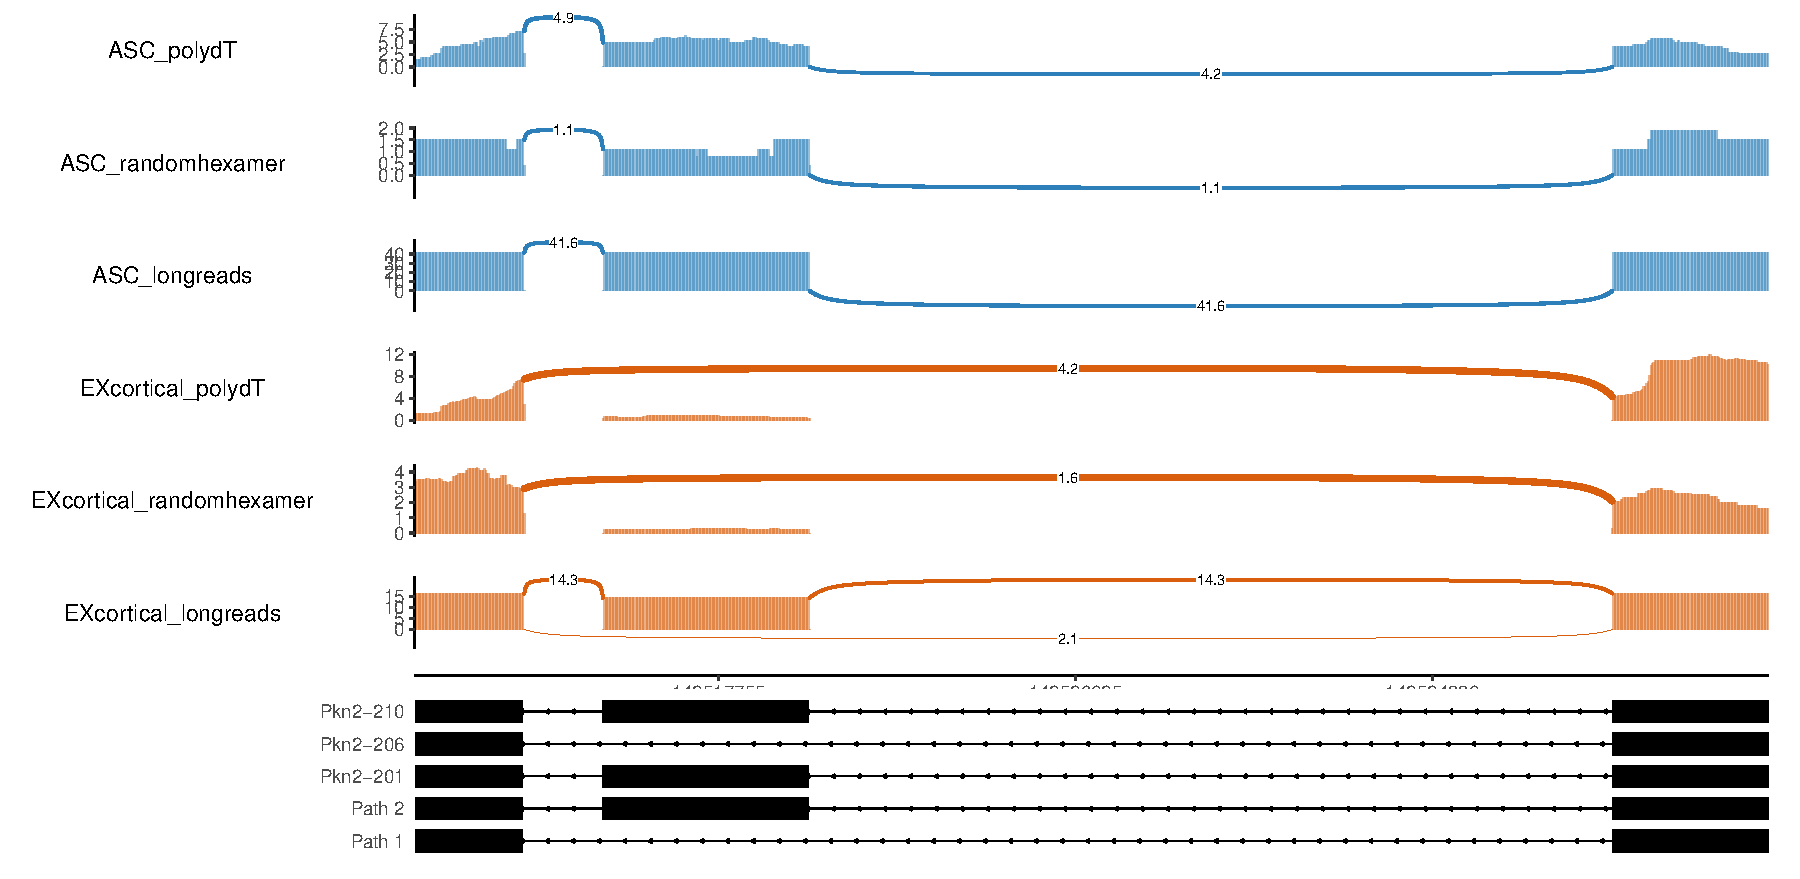
\includegraphics[width=0.8\textwidth]{figures/sashimi_Pkn2_B3.pdf}\end{minipage}\\[2pt]
\begin{minipage}[t]{0.45\textwidth}\vspace{0pt}\raggedright\panel{b}\\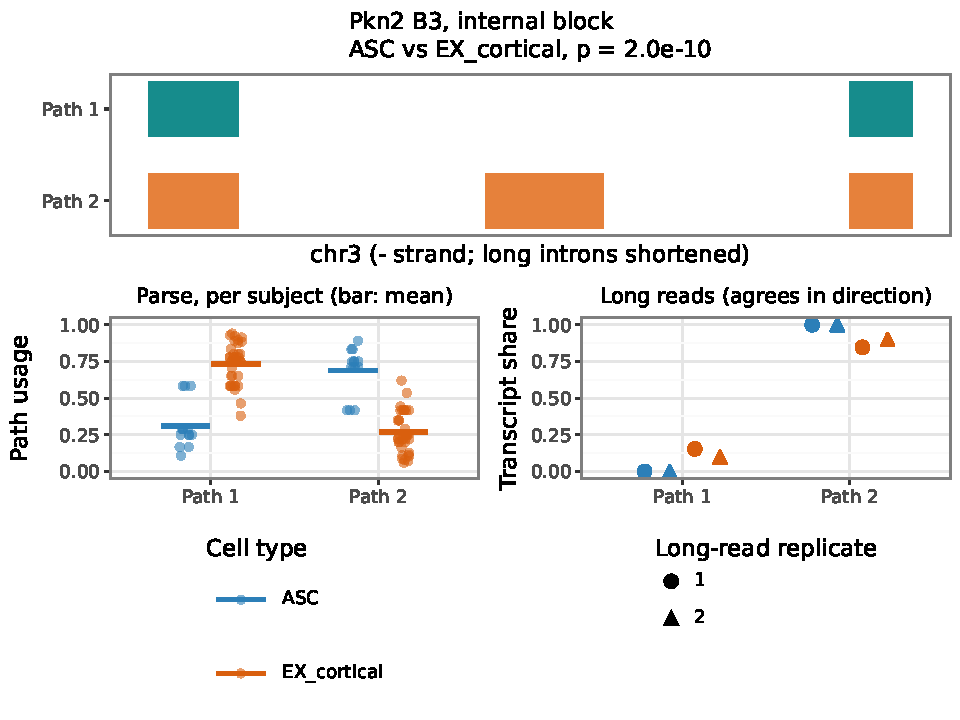
\includegraphics[width=\textwidth]{figures/example_Pkn2_B3.pdf}\end{minipage}\hfill
\begin{minipage}[t]{0.45\textwidth}\vspace{0pt}\raggedright\panel{d}\\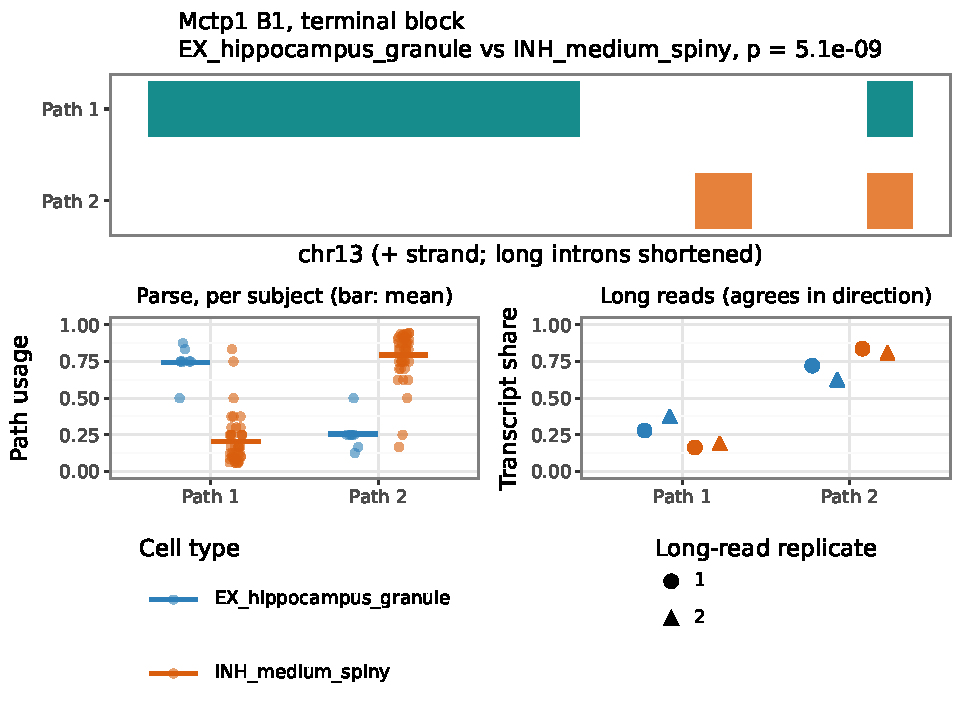
\includegraphics[width=\textwidth]{figures/example_Mctp1_B1.pdf}\end{minipage}\\[2pt]
\begin{minipage}{\textwidth}\raggedright\panel{c}\\\centering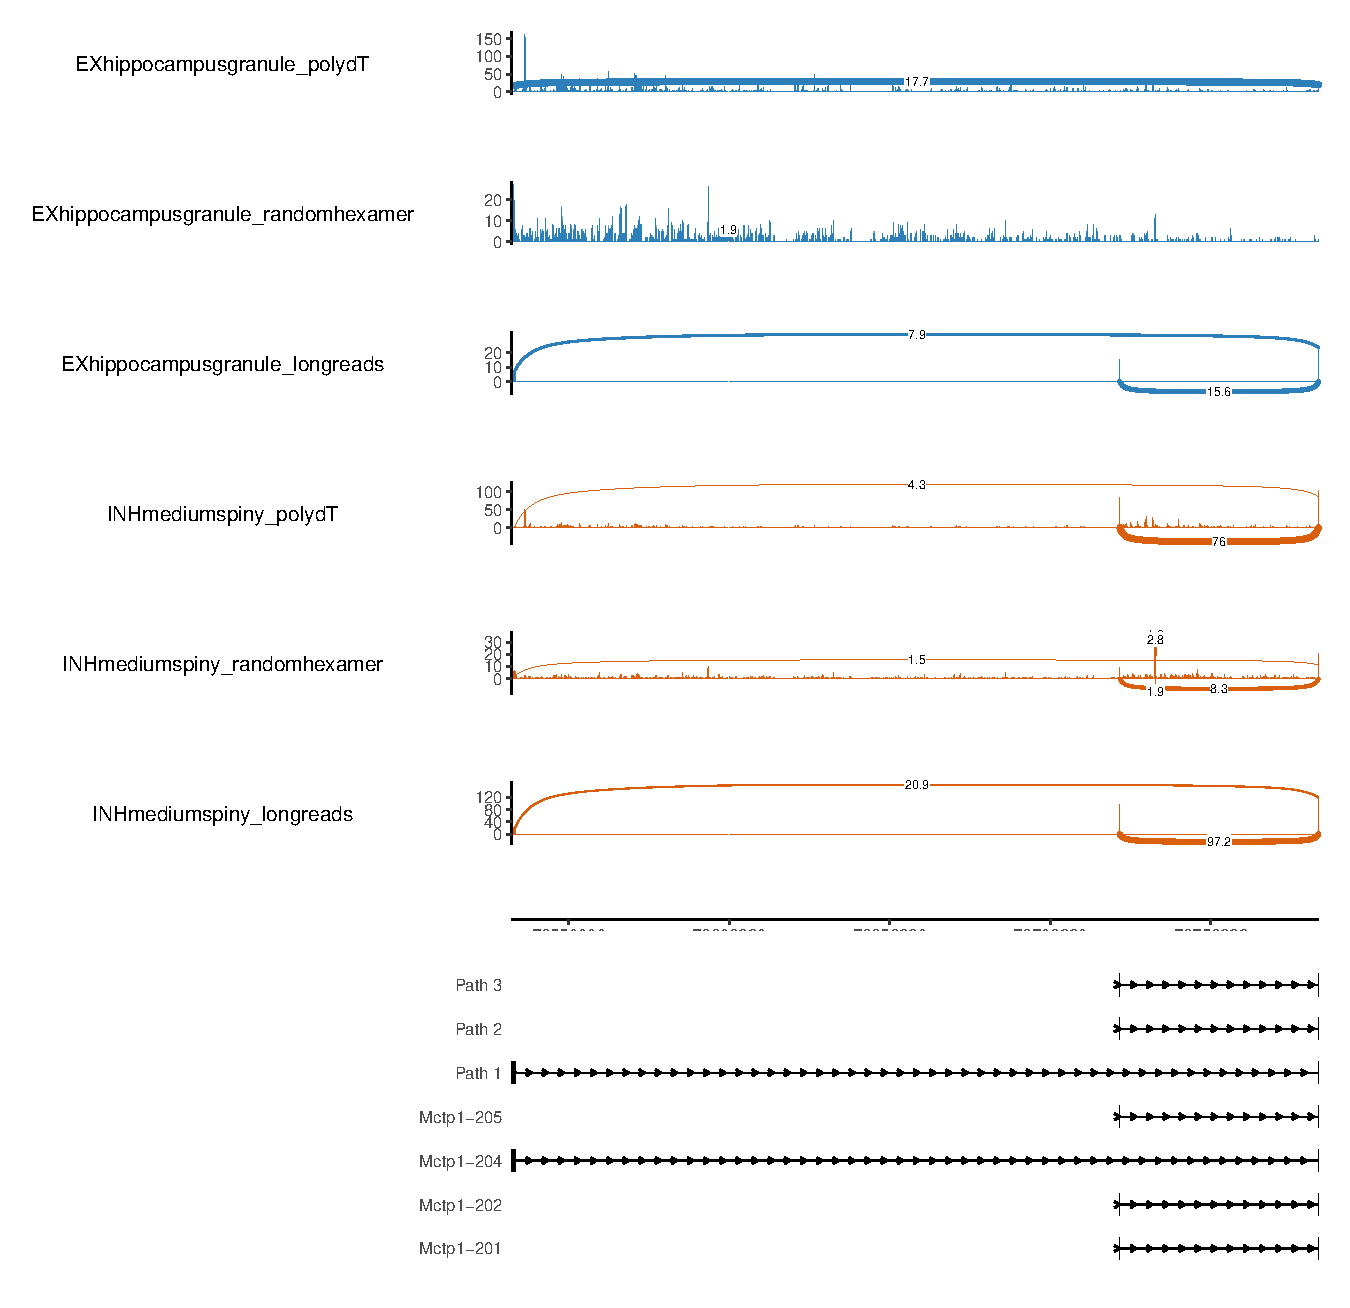
\includegraphics[width=0.8\textwidth]{figures/sashimi_Mctp1_B1.pdf}\end{minipage}
\caption{Examples in mouse brain. \textbf{a}, Sashimi plot of \emph{Pkn2} block 3, a cassette exon included by path 2, in astrocytes and cortical excitatory neurons: Parse coverage from UMI-deduplicated alignments by primer, per 1{,}000 half-cells of the primer, and long-read coverage implied by the UMI counts of annotated transcripts, per million long-read UMIs of the cell type. Arcs are junctions labelled with their coverage, and long introns are shortened; below are the block's paths and the gene's annotated transcripts. \textbf{b}, The tested paths (top), the path usage of each animal in the Parse data with the mean over animals (bottom left) and the transcript share of each path in the two long-read replicates (bottom right). \textbf{c},\textbf{d}, As \textbf{a},\textbf{b} for \emph{Mctp1} block 1, an alternative first exon in a terminal block, in dentate gyrus granule neurons and medium spiny neurons; paths 2 and 3 share their junctions and are merged in the junction-only test. Whole-gene views are in Supplementary Fig.~\ref{fig:gene-views}.}
\label{fig:examples}
\end{figure}

\subsection{Human blood}

Three public Parse datasets of peripheral blood mononuclear cells (PBMCs) were processed by the same pipeline with the GRCh38 genome and the GENCODE v49 basic annotation \cite{frankish2023}: GSE320507, 38 donors with long COVID (LTCS, 26), after recovery from COVID-19 (CONV, 5) and healthy controls (HC, 7), and two stimulation series of 12 and 8 donors, of which only the unstimulated or vehicle-control cells are used for cell-type contrasts. Cell types are CellTypist labels \cite{dominguezconde2022} (19, 10 and 8 types). Long-read directions come from a public PacBio Kinnex library made from a Parse PBMC library of other donors, for which we called cell barcodes, UMIs and the reverse-transcription primer from the reads (93\% of 148 million reads assigned to a cell; Methods).

In GSE320507, with 19 donors per half, 65 genes replicate between halves on the keys Tealeaf tests in both, and 91\% of the genes discovered in one half have $p\le0.05$ in the other (Supplementary Table~\ref{tab:pbmc}). Most replicated genes separate monocytes from lymphocytes. With 6 donors per half GSE327907 replicates 5 genes, and GSE334840, with 4 donors per half and 66-base reads, almost none. Of the 100 top-ranked long-read-evaluable tests, 99, 96 and 82 agree with the long reads in the three datasets (Fig.~\ref{fig:blood}c; Supplementary Table~\ref{tab:pbmc-lr}). Tests in blood reject less often than tests in brain at the same coverage, 2.4\% at $p<0.01$ in GSE320507 against 9.0\% in brain for rows with a median of 20 to 50 molecules, consistent with smaller splicing differences between blood cell types than between neuronal and glial cell types.

We ran the six comparators on GSE320507 as on the brain data, with the same coverage-only filter. In blood, LeafCutter and scQuint replicate about as many genes as Tealeaf on their universes (60 against 56 and 67 against 54; Fig.~\ref{fig:blood}a), and their top-ranked features agree with the long reads as often ($A_{100}$ 0.989 and 1.000 against 0.988; Fig.~\ref{fig:blood}b), over two to three times fewer evaluable tests (13{,}846 to 19{,}875 against 44{,}349). MAJIQ, after the removal of 96\% of its recomputed edges, replicates 26 genes against 68. rMATS replicates 133 genes against 60, but 64 of its 100 top-ranked events agree with the long reads, so most of its replicated genes are not supported by the long reads. SUPPA2 and primer-aware SUPPA2 replicate no genes and their top-ranked events agree at about chance, although SUPPA2 makes 65{,}760 discoveries on the 135 pairs every method tests (Supplementary Fig.~\ref{fig:discoveries-pbmc}).

\subsection{Tests between groups of donors}

GSE320507 also allows tests between disease groups within a cell type, where the two levels are different donors. Each cell type has four contrasts, LTCS against HC, LTCS against CONV, CONV against HC, and LTCS against HC and CONV pooled, and a fifth contrast compares two sets of 26 and 12 donors drawn at random, which has no group effect. The random contrast rejects below the nominal rate at $p<0.01$ and $p<0.001$ and has no discoveries (Fig.~\ref{fig:blood}d), so the test is not anticonservative with 12 donors in the smaller group. LTCS against HC gives 215 discoveries in 153 genes, mostly in naive and central-memory helper T cells and classical monocytes. The CONV donors share these differences. Of the 215 tests, 205 are also tested between CONV and HC, 59\% with $p<0.05$ and 92\% with the same direction, while LTCS against CONV has $p<0.05$ for 9\% (3\% for the random contrast). The differences therefore separate healthy donors from all donors after COVID-19, not long COVID from recovery, and may reflect other differences between the donor groups, such as age or time of sampling, which are not available. Fig.~\ref{fig:blood}e shows the discovery with the largest effect under the selection rule of Methods, a 69-base cassette exon of \emph{ANKRD12} in classical monocytes, included in 42\% of HC and 75\% of LTCS molecules; the other three examples are in Supplementary Figs.~\ref{fig:tcerg1}--\ref{fig:tc2n}.

\begin{figure}[p]
\centering
\begin{minipage}[t]{0.5\textwidth}\vspace{0pt}\raggedright\panel{a}\\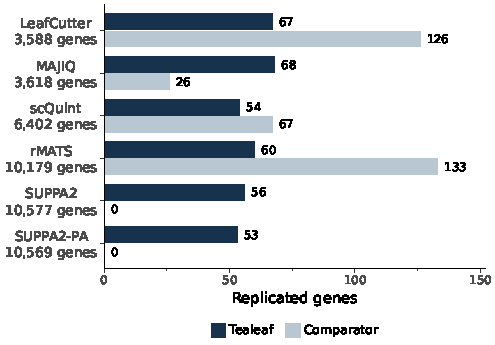
\includegraphics[width=\textwidth]{figures/paper/fig5_split.pdf}\end{minipage}\hfill
\begin{minipage}[t]{0.49\textwidth}\vspace{0pt}\raggedright\panel{b}\\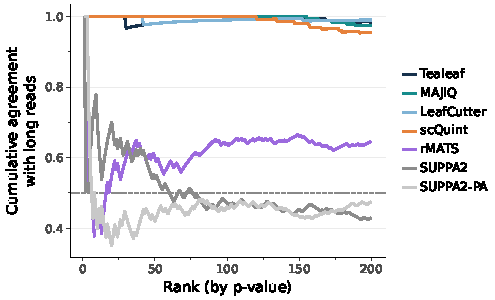
\includegraphics[width=\textwidth]{figures/paper/fig5_lr.pdf}\end{minipage}\\[4pt]
\begin{minipage}[t]{0.45\textwidth}\vspace{0pt}\raggedright\panel{c}\\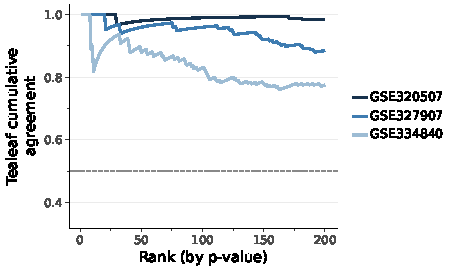
\includegraphics[width=\textwidth]{figures/paper/fig5_datasets.pdf}\end{minipage}\hfill
\begin{minipage}[t]{0.54\textwidth}\vspace{0pt}\raggedright\panel{d}\\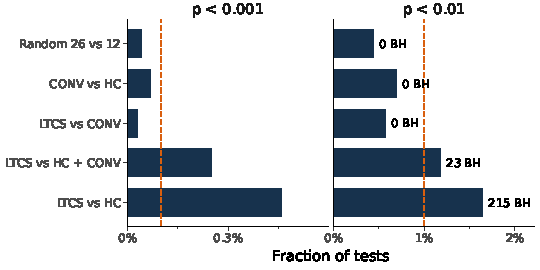
\includegraphics[width=\textwidth]{figures/paper/fig5_disease.pdf}\end{minipage}\\[4pt]
\begin{minipage}[t]{\textwidth}\vspace{0pt}\raggedright\panel{e}\\\centering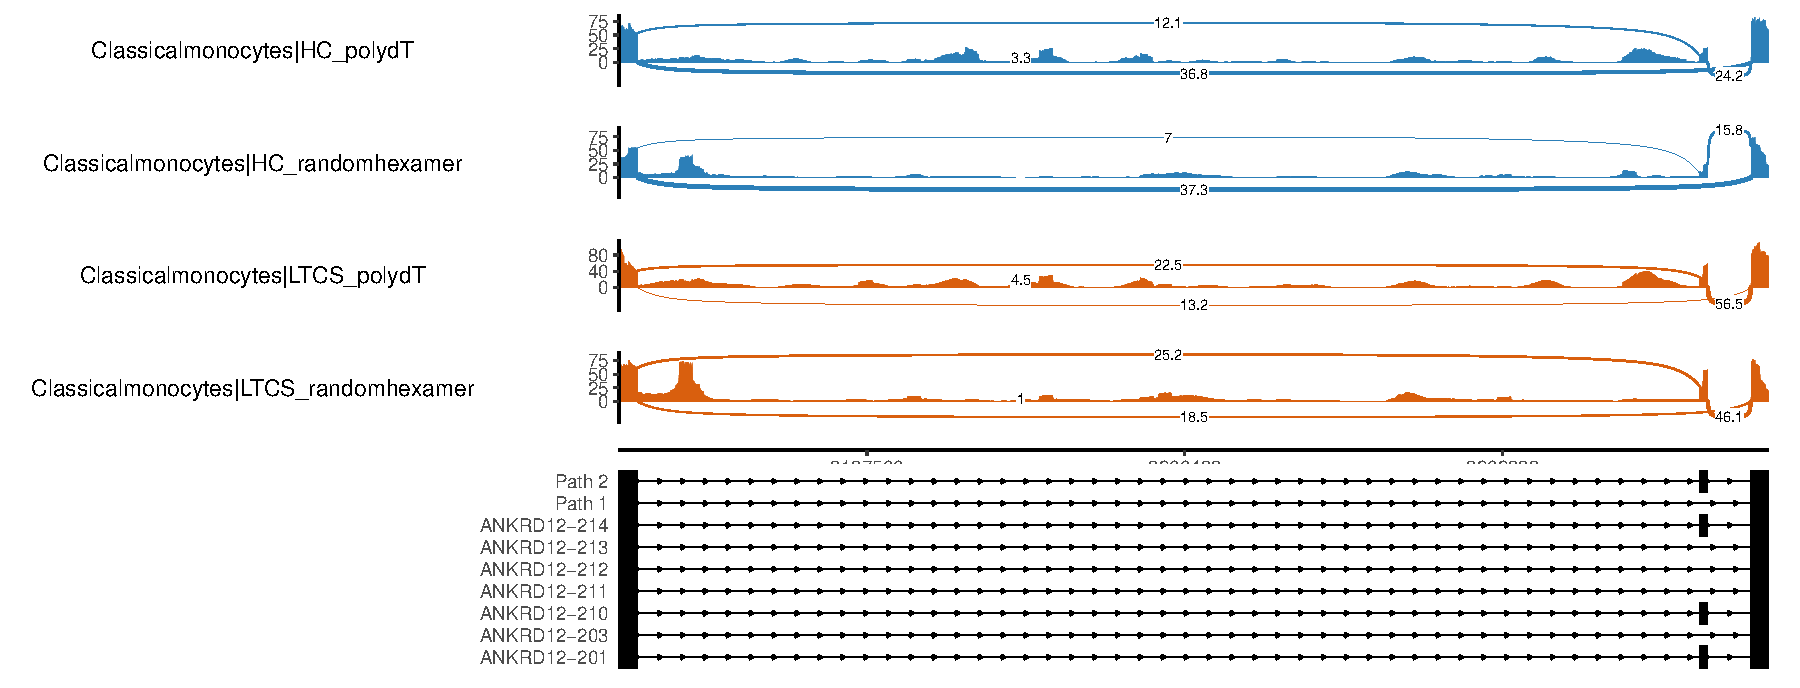
\includegraphics[width=0.85\textwidth]{figures/sashimi_ltcs_ANKRD12_B2.pdf}\end{minipage}
\caption{Human blood. \textbf{a}, Replicated genes in GSE320507 on each comparator's universe, as in Fig.~\ref{fig:brain}a. \textbf{b}, Cumulative agreement with the directions of the Kinnex Parse long reads in GSE320507, as in Fig.~\ref{fig:brain}b. \textbf{c}, Tealeaf cumulative agreement in the three PBMC datasets. \textbf{d}, Fraction of tests with $p<0.001$ and $p<0.01$ for disease-group contrasts within cell types in GSE320507, with the number of BH discoveries within each contrast; Random compares two sets of 26 and 12 donors drawn without regard to group. Dashed lines are the nominal rates. \textbf{e}, \emph{ANKRD12} block 2 in classical monocytes of HC (7 donors) and LTCS (26 donors): Parse coverage by primer per 1{,}000 half-cells, with the block's paths and the gene's annotated transcripts; the long-read library has no disease groups. Tests called by the coverage-only null are removed in \textbf{a} and \textbf{b} for every method except SUPPA2.}
\label{fig:blood}
\end{figure}

\section{Discussion}

Split-pool single-cell RNA-seq with random-hexamer priming observes splice junctions in transcript bodies across many cell types and donors. Tealeaf uses these data by testing local splice paths with every molecule that overlaps a block, both primers in one likelihood and donors as replicates. In mouse brain it replicates more genes across halves of the animals than six comparators, on each comparator's own universe, and its top-ranked directions agree with long reads as often as the best comparator's, over four to twenty-five times as many evaluable tests. Path tests cover alternative first and last exons and unannotated paths in the same framework as cassette exons, and these make up much of its discoveries.

Split replication rewards a test that responds to expression rather than splicing, because expression differences between cell types are shared by all donors and replicate across halves. Long-read direction is less affected, since such tests agree with the long reads at random, but it covers few genes. The coverage-only null addresses this for every method in the same way. It shows that most MAJIQ and many rMATS calls in these data arise from coverage alone, which a per-sample PSI estimate with a prior, or a test with too small a variance, does not separate from splicing. The filter removes such tests but cannot correct a test whose null distribution is too wide, and rMATS keeps more replicated genes than Tealeaf in blood with long-read agreement near 0.6. A comparison of splicing methods on single-cell data needs such a null, and replication alone is not sufficient.

In blood, LeafCutter and scQuint match Tealeaf on both endpoints in the largest dataset, and Tealeaf's advantage is the number of tests it can evaluate. Splicing differences between blood cell types are smaller than between neural cell types, and many blood genes have their alternatives at transcript ends, where Tealeaf uses junction-spanning molecules only. With few donors per half, as in the two stimulation series, few genes replicate for any test.

The evaluation has limits. The long-read data come from other animals or donors and cover eight brain and up to fourteen blood cell types, and the comparison is by direction only. Long reads from the same samples, with the same cell-type labels, would allow comparing effect sizes. Intron retention is tested separately, and with these data it is underpowered (Supplementary Note~\ref{sec:ir}). The disease contrasts in GSE320507 separate healthy donors from donors after COVID-19 and cannot be attributed to disease with the available sample information. Tealeaf's tests are calibrated in simulations on the real designs and in random contrasts between groups of donors, so they can be used for cohort designs in which donors, not cells, are the replicates.

\section{Methods}

\subsection{Mouse brain data and notation}

The brain data are split-pool barcoded single-nucleus RNA-seq (Parse Biosciences) of mouse brain, 48 subjects in six genotype or treatment groups (8 subjects each), in 8 sublibraries sequenced in 16 runs (about 345 million read pairs per run, 5.6 billion in total). Read 1 (151 bases) is cDNA in the sense orientation of the RNA. Read 2 carries the UMI at bases $[0,10)$ and three 8-base barcode segments at $[10,18)$, $[48,56)$ and $[78,86)$. Each cell is barcoded in one first-round well primed with poly(dT) and in one primed with random hexamers, so each cell has two \emph{half-cell} barcodes, one per primer. Cells are the annotated cells of the dataset (cell-type labels from the original clustering) whose pair of half-cell barcodes belongs to that cell only; a barcode pair shared by cells in different sublibraries cannot be resolved from the barcode and is excluded. Both halves of each cell are used, with no count threshold, giving 37{,}002 cells (74{,}004 half-cell barcodes) in 19 cell types, the cells of the comparator methods without the shared barcode pairs. A half-cell barcode determines its subject $u$, cell type $c$ and primer $p\in\{\mathrm{dT},\mathrm{hex}\}$.

Throughout, intervals are 0-based and half-open. A \emph{junction} $(d,a)$ is the intron $[d,a)$, where $d$ is the end of the donor exon and $a$ the start of the acceptor exon. For a block $b$ with $S_b$ mature paths, path $s\in\{1,\ldots,S_b\}$ is an exon chain $E_s=((x_{s1},y_{s1}),\ldots,(x_{sm_s},y_{sm_s}))$ with $m_s$ exons, and $J_s$ is its set of junctions $\{(y_{si},x_{s,i+1}):y_{si}<x_{s,i+1}\}$. The block window is $W_b=[\min_s x_{s1},\max_s y_{sm_s})$. A compatibility class $k$ is a non-empty subset of paths, encoded as a bit mask.

\subsection{Targeted reference and index}

\paragraph{Target loci.} The targets are the 33{,}755 genes with a multi-exon annotated transcript, so that genes without an annotated block of several paths can still receive blocks from unannotated junctions (Section~\ref{sec:novel}). Each gene span (GENCODE vM32 basic annotation, GRCm39), from the first to the last base of its annotated transcripts, is a target interval, and overlapping intervals are merged into a locus. The spans are not padded: novel junctions are used only inside annotated gene spans (Section~\ref{sec:novel}), so flanking sequence contributes no path, and padding each span by 1~kb changes fewer than 0.2\% of block molecules. This gives 26{,}612 loci with 1.19~Gb of sequence. The reference is the concatenation of the locus sequences and the spliced sequences of the 59{,}378 annotated transcripts of the target genes, separated by runs of 300 N, in a 2-bit code with N as a fifth symbol.

\paragraph{Index.} Every k-mer ($k=23$) without N that starts in a locus, and every transcript k-mer that spans an exon junction of its transcript, is indexed. The k-mer codes are sorted, and a table over the leading 24 bits of the code gives the range of each prefix. The index holds 1.19 billion k-mers.

\paragraph{Genome uniqueness.} The aligner sees only the target loci, so a read from a paralog or repeat elsewhere in the genome can align to a locus with a good score. Tealeaf replaces the genome-wide search for competing alignments by a uniqueness flag per indexed k-mer. The canonical code (the smaller of the code and the code of its reverse complement) of every k-mer of the genome is looked up in the index, and occurrences are counted. A locus k-mer is \emph{genome-unique} if its canonical code occurs exactly once in the genome; a transcript junction k-mer is genome-unique if it does not occur in the genome. 83.7\% of indexed k-mers are genome-unique. An alignment is accepted as unique only if one of its aligned blocks contains a k-mer that matches the read exactly and is genome-unique. A read from another genomic copy cannot contain such a k-mer unless a sequencing error creates it.

\subsection{Read alignment}

Each read $q\in\{0,1,2,3,4\}^L$ ($L=151$) is aligned in both orientations, $q$ and its reverse complement $\bar q$, and all candidate alignments of both orientations compete. Algorithm~\ref{alg:align} gives the procedure for one orientation. Scores follow STAR \cite{dobin2013}. For an alignment with $M$ matching and $X$ mismatching bases (read N bases are neutral), aligned blocks separated by junctions $j\in\mathcal J$ and indels $i\in\mathcal D$ of length $g_i$, and reference span $\ell$ (from the first to the last aligned base, introns included), \[\mathrm{score}=M-X+\sum_{j\in\mathcal J}\sigma(j)-\sum_{i\in\mathcal D}(2+2|g_i|)+\min\{0,\lceil-0.25\log_2\ell-0.5\rceil\},\] where the junction score is $\sigma(j)=+2$ for a known junction, $0$ for an unannotated GT/AG (or CT/AC) junction, $-4$ for GC/AG (CT/GC) and $-8$ for AT/AC (GT/AT). A gap of at least 21 bases between consecutive blocks is a junction; shorter gaps of at most 6 bases are deletions (positive gap) or insertions (negative gap).

\begin{algorithm}[ht]
\caption{Alignment candidates of one read orientation $q$ of length $L$.}
\label{alg:align}
\begin{algorithmic}[1]
\State \textbf{Seeds.} For read positions $r=0,4,8,\ldots$ and $r=L-k$, look up the k-mer $q[r,r+k)$ unless it contains N; keep hits of k-mers with at most 32 index occurrences (at most 1{,}024 hits). Each hit at reference position $t$ has diagonal $\delta=t-r$.
\State \textbf{Segments.} Merge hits with equal $\delta$ into segments $(\delta,r_{\rm start},r_{\rm end})$ spanning the read positions of their k-mers.
\For{each segment on a transcript}
  \State Extend ungapped along the transcript in both directions (X-drop, at most 10 mismatches in total); project the aligned read interval onto the transcript's exons to give genomic blocks; add as a candidate.
\EndFor
\State \textbf{Chaining.} Sort locus segments by $r_{\rm start}$. Dynamic programming, $D_j=r^{\rm end}_j-r^{\rm start}_j$, and for each predecessor $i$ in the same locus with $r^{\rm start}_i<r^{\rm start}_j$, $r^{\rm end}_i\le r^{\rm end}_j$ and diagonal gap $g=\delta_j-\delta_i\in[-6,-1]\cup[1,6]\cup[21,10^6]$, $D_j\gets\max\{D_j,D_i+r^{\rm end}_j-\max(r^{\rm start}_j,r^{\rm end}_i)\}$.
\For{each chain end in decreasing $D$, not yet used, with $D\ge k$}
  \State Trace the chain back; extend its first segment to the left (X-drop, at most 10 mismatches).
  \For{consecutive segments $A,B$ of the chain}
    \State Choose the split $s$ within 4 bases of the segment boundary that minimizes mismatches of $q[\cdot,s)$ on $\delta_A$ and $q[s,\cdot)$ on $\delta_B$; for a junction ($g\ge21$) require a known junction or a canonical motif, and break ties by known, then GT/AG, then other canonical motifs.
  \EndFor
  \State Extend the last segment to the right with the remaining mismatch budget.
  \State \textbf{Rescue.} If the right end is soft-clipped by at least 3 bases, try junctions from split points $s$ within 6 bases of the clip to every known acceptor $a$ at intron length 21 to $10^6$; an unknown junction needs a canonical motif and a tail of at least 5 bases. Accept the best split whose tail has at most $\max(1,\lfloor (L-s)/10\rfloor)$ mismatches and whose score gain over clipping is positive. Do the same for a clipped left end and every known donor.
  \State Add the alignment as a candidate.
\EndFor
\end{algorithmic}
\end{algorithm}

\paragraph{X-drop extension.} An extension from a seed boundary scores $+1$ per match and $-1$ per mismatch, stops when the score falls 8 below its maximum, at an N in the reference, at the locus or transcript boundary, or at the mismatch budget, and ends at the position of the maximum. The unaligned remainder is soft-clipped.

\paragraph{Overhang minimum and candidate scoring.} Before scoring, a terminal block shorter than the minimum overhang of its junction is removed, as with STAR's \texttt{alignSJDBoverhangMin} and \texttt{alignSJoverhangMin}, 3 bases for a known junction and 5 for an unannotated one. Candidates with identical reference start, end, block count and orientation are merged keeping the higher score. A table holds at most 24 candidates; when it is full, a new candidate replaces the lowest-scoring one if it scores higher.

\paragraph{Read status.} Let $c^\star$ be the highest-scoring candidate over both orientations. The read is
\begin{enumerate}[leftmargin=*]
  \item \emph{too short} if $\mathrm{score}(c^\star)<\lfloor0.66(L-1)\rfloor$, $M(c^\star)<\lfloor0.66(L-1)\rfloor$, $X(c^\star)>10$ or $X(c^\star)>0.3(M+X)$;
  \item \emph{multi-mapping} if another candidate scores at least $\mathrm{score}(c^\star)-1$ and does not overlap $c^\star$ on the reference, or lies on the other orientation;
  \item \emph{not genome-unique} if no aligned block of $c^\star$ contains an exactly matching genome-unique k-mer;
  \item \emph{unique} otherwise.
\end{enumerate}
Only unique alignments are used. The aligned blocks of $c^\star$ are mapped back to genomic coordinates.

\paragraph{Two passes.} The first pass uses the annotated junctions of the target transcripts as known junctions. For each run, the junctions of unique alignments are counted with the largest overhang (shorter flanking block) among their reads. An annotated junction is kept; an unannotated one is kept if its largest overhang is at least 12 bases and it has at least 4 reads, or 3 reads and an intron of at most 200~kb, 2 reads and at most 100~kb, or 1 read and at most 50~kb (STAR's \texttt{outSJfilter} defaults for canonical motifs). The intron strand is the strand of the motif. Counts are summed over runs, and for each junction the number of sublibraries with reads is recorded. These counts use every uniquely aligned read, irrespective of its barcode, and never use cell-type labels. The second pass adds to the known junctions every first-pass junction with a canonical motif, at least 20 reads and at least 4 of the 8 sublibraries, the support required of a novel path (Section~\ref{sec:novel}); junction counts from the second pass then define the novel paths. Known junctions receive the $+2$ score, the 3-base overhang minimum and the rescue of clipped ends, as in STAR's two-pass mode.

\subsection{Cell barcodes, UMIs and molecules}

Each 8-base barcode segment of read 2 is corrected to its 96-entry whitelist, by replacing it with the unique nearest whitelist entry within Hamming distance 2 (N read as T); a segment without such an entry is uncorrectable. A read is assigned to a half-cell barcode if all three segments correct and the triple is the barcode of a retained cell in its sublibrary. Its UMI is valid if it contains no N and is not a homopolymer. Unique alignments with an assigned barcode and a valid UMI are kept.

Within each (half-cell barcode, locus), UMIs at Hamming distance 1 are joined transitively and replaced by the smallest UMI of their component (STARsolo's \texttt{1MM\_All}). A \emph{molecule} is a (half-cell barcode, collapsed UMI, block) triple, over the reads of both sequencing runs of a sublibrary.

\subsection{Splice blocks and paths}

\subsubsection{Annotated blocks}
\label{sec:blocks}

Annotated splice blocks are local regions between constitutive exonic anchors in the annotation. Transcripts of a gene that take the same exon chain through the region are collapsed into one path, and a block has the paths of all annotated transcripts that traverse it. Each path is the chain left anchor exon, internal exons, right anchor exon, with exons that touch merged into one, so transcripts whose chains differ only by an exon boundary inside a continuous exonic interval share a path. A path whose chain is the whole window duplicates the precursor path below and is removed. Blocks of the target genes with 2 to 30 annotated paths are used. Every block also carries a \emph{precursor} path, the single exon $W_b$, which is compatible with reads without a junction inside the window (intronic or exon-body reads).

A block is \emph{internal} if all its annotated paths start with the same exon and end with the same exon, and \emph{terminal} otherwise (alternative first or last exons, transcript starts or ends). The structure is decided from the annotated paths only, so adding novel paths does not change it.

\subsubsection{Novel paths}
\label{sec:novel}

Novel paths are built from the second-pass junction support. For a block $b$, let $\mathcal A_b=\bigcup_sJ_s$ be its annotated junctions, $R(j)$ and $\Lambda(j)$ the read count and number of sublibraries of junction $j$, and $R_b^\star=\max_{j\in\mathcal A_b}R(j)$. A junction $(d,a)\notin\mathcal A_b$ is a \emph{novel junction} of $b$ if $d,a\in W_b$, its intron strand is the gene's strand, and \[R(d,a)\ge\max\{20,\,0.02R_b^\star\},\qquad \Lambda(d,a)\ge4.\] For an annotated path $E$, the donor $d$ attaches to exon $i$ of $E$ if $x_i<d\le y_i$ (an earlier donor within the exon) or $y_i<d<x_{i+1}$ with $d-y_i\le300$ (an exon extension into the intron); the acceptor $a$ attaches to exon $j$ if $x_j\le a<y_j$ or $y_{j-1}<a<x_j$ with $x_j-a\le300$. Novel junctions modify one annotated path each, by the rules of Algorithm~\ref{alg:novel} and Supplementary Fig.~\ref{fig:novel}. At most 8 novel paths are kept per block, ordered by the smallest read count of their novel junctions, and a novel path identical to an annotated one is discarded.

\begin{algorithm}[ht]
\caption{Novel paths of block $b$ from its novel junctions $\mathcal N_b$; $T=151$ is the new terminal exon length.}
\label{alg:novel}
\begin{algorithmic}[1]
\State \textbf{Pairs.} For novel junctions $(d,x),(y,a)\in\mathcal N_b$ with $d<x<y<a$ and $y-x\le1{,}000$, form the candidate $(d,a)$ with new exon $[x,y)$; mark both junctions as paired.
\State \textbf{Singles.} Every $(d,a)\in\mathcal N_b$ is also a candidate without a new exon.
\For{each candidate and each annotated path $E$}
  \If{$d$ attaches to exon $i$ and $a$ to exon $j\ge i$ of $E$}
    \State New chain: exons $1..i-1$ of $E$, $(x_i,d)$, the new exon if any, $(a,y_j)$, exons $j+1..m$ of $E$. A single that is paired may not use an exon extension.
  \ElsIf{the candidate is an unpaired single, $d$ attaches to no exon of $E$ and $a$ attaches to exon $j$}
    \State New first exon: $(\max\{d-T,\,y^-\},d)$, then $(a,y_j)$ and exons $j+1..m$, where $y^-$ is the largest exon end of $E$ before $d$ (or the window start).
  \ElsIf{the candidate is an unpaired single, $d$ attaches to exon $i$ and $a$ to no exon of $E$}
    \State New last exon: exons $1..i-1$, $(x_i,d)$, then $(a,\min\{a+T,\,x^+\})$, where $x^+$ is the smallest exon start of $E$ after $a$ (or the window end).
  \EndIf
\EndFor
\State For each candidate, keep the chain from the path where it replaces a junction sharing its donor or acceptor, then with the least exon extension, then whose least supported junction has most reads.
\end{algorithmic}
\end{algorithm}

\paragraph{New blocks.} Novel junctions inside a gene that lie in no annotated block window, for example a junction that skips an exon constitutive in the annotation, define new blocks. Such a junction is used if it satisfies the support criteria above, with $R^\star$ the largest read count of the annotated junctions overlapping it. Used junctions with overlapping introns are clustered. For a cluster with first donor $d$ and last acceptor $a$, each annotated transcript gives the segment of its exon chain from the exon to which $d$ attaches to the exon to which $a$ attaches; if only one end attaches, the segment starts at the last exon ending before $d$ or ends at the first exon starting after $a$, which allows novel first and last exons. Segments are clipped to their shared extent, distinct clipped segments are the annotated paths of the new block, and Algorithm~\ref{alg:novel} adds its novel paths. A new block is kept if it has at least one novel path.

\paragraph{Block set.} On the second pass the block set has 34{,}677 blocks, 22{,}898 annotated and 11{,}779 new, with 21{,}509 novel paths.

\subsection{Molecule classes}
\label{sec:classes}

\paragraph{Read compatibility.} For a read with aligned blocks $\{[\alpha_r,\beta_r)\}$ and junctions $\mathcal J_{\rm read}$, and a block $b$ whose window it overlaps, the read's blocks are clipped to $W_b$ and its junctions restricted to those inside $W_b$. The read is compatible with path $s$ (or the precursor path) if every clipped block lies within one exon of $E_s$ and every junction inside the window belongs to $J_s$. The read's class in block $b$ is the mask of compatible paths. A read of class 0, compatible with no path (for example a read with an unannotated junction not represented by a novel path, or a block reaching into an intron), is left out of the block. A molecule's class is the bitwise AND of the classes of its remaining reads that overlap the window; a molecule whose reads are compatible with disjoint sets of paths has class 0 and is discarded. A read enters every block of its locus whose window it overlaps.

\paragraph{Junction-only classes.} A junction is \emph{variable} in block $b$ if it belongs to some but not all mature paths. The junction-only collection keeps a molecule only if at least one of its reads of non-zero class has a variable junction inside the window.

\paragraph{Counts.} For each block, molecule counts are summed over the half-cell barcodes of each (subject, cell type, primer) and over sublibraries, giving $y_{ucpk}\in\mathbb N_0$ for subject $u$, cell type $c$, primer $p$ and class $k$. Internal blocks use the all-read counts and terminal blocks the junction-only counts.

\subsection{Read opportunities}

The probability of each class given the path composition is determined by read geometry. For path $s$ with spliced length $\lambda_s=\sum_i(y_{si}-x_{si})$, consider a read of length $L=151$ starting at every position $t\in\{1-L,\ldots,\lambda_s-1\}$ of the path's spliced sequence, so that it overlaps the path by at least one base, with the part outside the path clipped, as reads leaving the window are clipped in the data. The read's spliced interval is mapped to genomic blocks and junctions and classified with the same compatibility rule. The opportunity $n_{ks}\in\mathbb N_0$ is the number of start positions on path $s$ that give class $k$, and $L_s=\sum_kn_{ks}$ is the effective length of path $s$. For junction-only classes, only start positions whose read spans a variable junction count. Opportunities are computed for the $S_b$ mature paths and the precursor path.

Under a model in which molecules of path $s$ arise in proportion to an abundance $\rho_s$ per position and start uniformly along it, $P(\text{class }k)=\sum_s\rho_sn_{ks}/\sum_s\rho_sL_s$. The molecule share of path $s$ is $\pi_s=\rho_sL_s/\sum_{s'}\rho_{s'}L_{s'}$.

\subsection{Block test}
\label{sec:block}

\subsubsection{Projection and screens}

A test is indexed by a block $b$ and an unordered pair of cell types $\{c_0,c_1\}$, with $c_0$ the first in alphabetical order; effects are reported as $c_1$ minus $c_0$. The data of a test are the counts $y_{ucpk}$ for $c\in\{c_0,c_1\}$.
\begin{enumerate}[leftmargin=*]
  \item \textbf{Eligibility.} At least 4 subjects have molecules in both cell types, and the block has at least 20 molecules in the two cell types.
  \item \textbf{Same-junction groups (terminal blocks).} Paths with identical junction sets cannot be separated by junction-spanning reads and are merged into one group. A class is compatible with a group if it is compatible with any member, and the group opportunity is the mean of its members' opportunities. A block with fewer than two groups is not tested.
  \item \textbf{Share screen.} Molecule shares $\widehat{\bm\pi}$ are estimated from the class counts pooled over both cell types, both primers and all subjects, by the EM algorithm for $P(k)=\sum_s\pi_sn_{ks}/L_s$, with a pseudocount of 0.5 molecules per path per iteration (tolerance $10^{-10}$, at most 1{,}000 iterations). For internal blocks the precursor path is a component of the EM and is removed afterwards, with the mature shares renormalized. Paths with $\widehat\pi_s<0.01$ are removed. A block with fewer than two remaining paths is not a hypothesis and leaves the family. The screen uses no cell-type labels within the pair.
  \item \textbf{Projection.} Masks are restricted to the retained mature paths and the precursor bit is dropped. Molecules compatible only with the precursor or only with removed paths are discarded; classes that become identical are merged, with opportunities summed. The eligibility criteria are then applied again to the projected counts.
\end{enumerate}
After projection let $S$ be the number of retained paths and $K$ the number of classes.

\subsubsection{Likelihood of one path against the rest}

For target path $s$, the other paths are collapsed into one component with weights \[w_j=\frac{\widehat\pi_j/L_j}{\sum_{j'\ne s}\widehat\pi_{j'}/L_{j'}},\qquad j\neq s,\] the per-position abundances implied by the pooled molecule shares, so that the collapsed component's molecules divide among its paths in proportion to $\widehat\pi_j$. For class $k$ let \[\beta_k=n_{ks},\qquad \eta_k=\sum_{j\ne s}w_jn_{kj},\qquad B=\sum_k\beta_k,\qquad H=\sum_k\eta_k.\] All classes are kept, including the class compatible with all paths, whose relative frequency informs $\psi$ through coverage. For a subject--cell-type row $(u,c)$ with target usage $\psi\in(0,1)$, the class probabilities in primer $p$ are \[f_{pk}(\psi)=\frac{\psi_p\beta_k+(1-\psi_p)\eta_k}{\psi_pB+(1-\psi_p)H},\qquad \psi_p=\expit(\logit\psi+\gamma_p),\] with $\gamma_{\rm dT}=0$ and $\gamma_{\rm hex}=\gamma$, a primer offset that absorbs differences in positional capture between the primers. $\psi$ is the target's share of per-position abundance (the $\rho$ scale of the previous section), so its expected molecule share in primer $p$ is $\psi_pB/\{\psi_pB+(1-\psi_p)H\}$. Conditioning on the primer totals, the row log-likelihood is \[\ell_{uc}(\psi)=\sum_{p\in\{\mathrm{dT},\mathrm{hex}\}}\sum_{k=1}^Ky_{ucpk}\log f_{pk}(\psi).\] 
\paragraph{Primer offset.} $\gamma$ is estimated before the test without cell-type labels, by maximizing the profile likelihood in which every row has its own usage, \[\widehat\gamma=\arg\max_{\gamma\in[-4,4]}\sum_{(u,c)}\max_{t\in\mathbb R}\left[\ell_{uc,\mathrm{dT}}(\expit t)+\ell_{uc,\mathrm{hex}}(\expit(t+\gamma))\right],\] over rows observed with both primers, where $\ell_{uc,p}$ is the primer-$p$ term of $\ell_{uc}$. The maximization uses a grid of step 0.05 in $\gamma$ and in $t\in[-22,22]$, refined by a parabola through the three best points. $\widehat\gamma$ is estimated for each target path and held fixed in both hypotheses.

\subsubsection{Random-effects model}

Let $z_c=\mathbf 1[c=c_1]$. Usage varies between subjects through a subject intercept and between rows through a Beta distribution, \[v_u\sim\mathcal N(0,\sigma^2),\qquad \mu_{uc}=\expit(\theta_0+\theta_1z_c+v_u),\qquad \psi_{uc}\mid v_u\sim\BetaDist\big(\kappa\mu_{uc},\kappa(1-\mu_{uc})\big),\] with fixed effects $\theta_0,\theta_1\in\mathbb R$, subject standard deviation $\sigma>0$ and row concentration $\kappa>0$. The subject intercept is shared by the subject's two cell types, which makes the test paired. Subjects observed in only one cell type contribute to $\theta_0$, $\sigma$ and $\kappa$. The marginal likelihood is \[\mathcal L(\theta_0,\theta_1,\kappa,\sigma)=\prod_u\int_{\mathbb R}\phi(v;0,\sigma^2)\prod_{c\in\mathcal C_u}\int_0^1e^{\ell_{uc}(\psi)}\,\BetaDist\big(\psi;\kappa\mu_{uc}(v),\kappa(1-\mu_{uc}(v))\big)\,d\psi\,dv,\] where $\mathcal C_u$ is the set of cell types observed for subject $u$.

\paragraph{Levels in different subjects.} The two levels of a test can also be groups of different subjects within one cell type, such as disease groups (Section~\ref{sec:pbmc}). Each subject then has one row, and $z_u$ indicates the subject's group. The model and test are unchanged; the subject intercept and the row Beta distribution both describe variation between subjects of a group. Eligibility requires a minimum number of subjects with molecules in each level instead of in both.

\paragraph{Numerical integration.} The inner integral is evaluated in $t=\logit\psi$ on $[-18,18]$ by the trapezoid rule, with the tails beyond $\pm18$ added analytically at the boundary value of $\ell_{uc}$. The grid spacing for row $(u,c)$ is $\min\{0.03,\,s_{uc}/1.5\}$, where $s_{uc}$ is a quarter of the width of the region where $\ell_{uc}(\expit t)$ is within 2 of its maximum. The outer integral uses adaptive Gauss--Hermite quadrature with 9 nodes, centred on each subject's posterior mode $\widehat v_u$ (damped Newton iterations) and scaled by the inverse square root of the negative second derivative of the log integrand at the mode.

\paragraph{Estimation.} Maximum-likelihood estimates are found by the L-BFGS-B algorithm with analytic gradients in the coordinates $(\theta_0,\theta_1,\log\kappa,\log\sigma)$, within the bounds $-12\le\theta_0,\theta_1\le12$, $0.1\le\kappa\le2000$ and $0.01\le\sigma\le3$. The null fit ($\theta_1=0$) starts from least-squares coefficients on the rows' maximum-likelihood usages, $\kappa=20$ and $\sigma=0.5$; the alternative starts from the null solution, and is refitted from $\theta_1=0$ if it ends below the null log-likelihood.

\paragraph{Test.} With $(\widehat\theta_0,\widehat\theta_1,\widehat\kappa,\widehat\sigma)$ the alternative and $(\widetilde\theta_0,0,\widetilde\kappa,\widetilde\sigma)$ the null estimates, the statistic is \[T_s=2\left\{\log\mathcal L(\widehat\theta_0,\widehat\theta_1,\widehat\kappa,\widehat\sigma)-\log\mathcal L(\widetilde\theta_0,0,\widetilde\kappa,\widetilde\sigma)\right\},\] and $p_s=P(\chi^2_1>T_s)$. Both optima are re-evaluated at half the $\psi$ grid spacing and 19 quadrature nodes; if the log-likelihoods or the statistic change by more than $10^{-3}$, the test is refitted at the finer setting and checked again at quarter spacing and 39 nodes. A test is converged if both fits succeed and the change is at most $10^{-3}$; the reported statistic is $\max(T_s,0)$ at the finer setting. A path test that does not converge has $p_s=1$.

\subsubsection{Block p-value and effect}

For $S=2$ there is one test, of path 1. For $S>2$, each of the $S$ paths is tested against the rest and the block p-value is the Simes combination \cite{simes1986} \[p_b=\min\left\{1,\ \min_{i=1,\ldots,S}\frac{S\,p_{(i)}}{i}\right\},\] where $p_{(1)}\le\cdots\le p_{(S)}$ are the ordered path p-values. The effect for $S=2$ is $\bar m_{c_1}-\bar m_{c_0}$ for path 1 (and its negative for path 2), where $\bar m_c=\int\expit(\widehat\theta_0+\widehat\theta_1z_c+v)\phi(v;0,\widehat\sigma^2)\,dv$ is the marginal usage on the poly(dT) scale. For $S>2$, the molecule-share composition of each row is estimated by the EM algorithm of the share screen with primers pooled, compositions are averaged over the subjects observed in both cell types (over the subjects of each level when the levels are groups of different subjects), and the effect is the difference of the averages.

\subsubsection{Hypothesis family}

Internal-block tests and terminal-block tests form one family, with BH applied over all tests of a cohort. A test that fails to converge, or has fewer than four subjects in its fit, enters with $p=1$; a block removed by a screen does not enter.

\subsection{Calibration}
\label{sec:calibration}

Calibration is checked by count simulations under the null on real designs. For randomly chosen blocks and cell-type pairs of the full data (200 for internal and 800 for terminal blocks, on the 1{,}163-gene block set of an earlier target list), the observed molecule totals per (subject, cell type, primer) are kept, and class counts are redrawn from compositions in which the two cell types share the same path usage. A subject composition is drawn from a Dirichlet distribution with concentration 20 around the pooled shares, the row composition from a Dirichlet with concentration $\varsigma\in\{5,20,\infty\}$ around the subject composition, and class counts from the multinomial implied by the opportunities, two draws per test. Internal tests reject at most 2.9\% of converged fits at nominal 0.05 and at most 1.0\% at 0.01. Junction-only terminal tests reject 3.4--4.3\% (two-path) and 2.7--4.1\% (multi-path) at 0.05, at most 1.1\% at 0.01 and at most 0.5\% at 0.001.

\subsection{Human blood data}
\label{sec:pbmc}

Three public Parse datasets of human peripheral blood mononuclear cells (PBMCs) were processed by the same pipeline as the brain data, with the GRCh38 genome and the GENCODE v49 basic annotation, all multi-exon genes as targets, two alignment passes and novel paths. A leading template-switch oligo is removed from read 1 before alignment, since on short reads the remainder would fall below the minimum aligned length.
\begin{enumerate}[leftmargin=*]
  \item \textbf{GSE320507} (Ray et al.\ 2026), PBMCs of donors with long COVID (LTCS), convalescent donors (CONV) and healthy controls (HC). Each sample occupies one first-round well. The well-to-donor map provided by the authors agrees with genotypes called from expressed variants in every well but one, which holds cells of two donors and is excluded. This leaves 38 donors (26 LTCS, 5 CONV, 7 HC).
  \item \textbf{GSE327907}, PBMCs of 12 donors in two batches under 12 in-vitro conditions; only the unstimulated cells enter the cell-type contrasts.
  \item \textbf{GSE334840}, PBMCs of 8 donors in two hormone treatments and a vehicle control (DMSO); only the control cells enter the cell-type contrasts.
\end{enumerate}
Cell types are CellTypist \cite{dominguezconde2022} labels with majority voting, from the fine-grained immune model for GSE320507 (19 types) and from the coarse model for the stimulation series, with macrophages merged into monocytes (10 and 8 types), because fine-grained labels separate stimulated monocytes by stimulus. Every pair of cell types is tested, and BH is applied over the internal and terminal tests of the cell-type pairs of a cohort. Donors are split into halves stratified by group (GSE320507) or batch (GSE327907). With no comparator fitted, the split universe is the set of (gene, cell-type pair) keys with a Tealeaf test in both halves, and replication is scored as in Section~\ref{sec:evaluation}.

Long-read directions come from a public PacBio Kinnex library made from a Parse whole-transcriptome library of commercial PBMCs, from donors other than those of the three datasets. The library provides segmented reads without cell calls, so the three barcodes, the UMI and the reverse-transcription primer of each read are called here. The two linkers are placed by semi-global alignment, each barcode is corrected to the unique barcode within edit distance 1, and the poly(T) and the template-switch oligo are trimmed. Of 148 million reads, 93\% are assigned to a cell. Reads are aligned to the genome with minimap2 \cite{li2018b} in spliced mode with the annotated junctions as hints. A read with mapping quality at least 5 is assigned to the gene with which it has the largest same-strand exonic overlap, and reads of a cell and gene whose UMIs differ by at most one base form a molecule, which takes the most frequent exon chain of its reads. Cells with at least 1{,}000 reads (10{,}077 cells, 26.4 million molecules) are labelled by CellTypist with the model used for each short-read dataset.

In GSE320507 the disease groups are compared within each cell type, with the levels in different donors (Section~\ref{sec:block}) and at least 4 donors in each level. Each cell type has four contrasts, LTCS against HC, LTCS against CONV, CONV against HC, and LTCS against HC and CONV pooled. A fifth contrast compares two sets of 26 and 12 donors drawn at random from the 38 without regard to group, the same draw in every cell type. Discoveries are BH-adjusted $p\le0.05$ within each contrast over its internal and terminal tests, with tests that do not converge entering at $p=1$. In the long-read data, cell types with at least one evaluable test are used, and directions are scored as in Section~\ref{sec:evaluation}.

\subsection{Evaluation in mouse brain}
\label{sec:evaluation}

\subsubsection{Subject-split replication}

The 48 subjects are divided into two halves of 24 with 4 subjects of each group in each half (subjects shuffled within group and assigned alternately). Tealeaf and every comparator are fitted separately on each half. For each comparator $m$, the universe $\mathcal K_m$ is the set of (gene, cell-type pair) keys with a finite p-value for $m$ in both halves, taken from the comparator's own results, over up to 190 cell-type pairs; no Tealeaf result enters it. SUPPA2 and primer-aware SUPPA2 use exact paired signed-rank tests over the full event catalogue. Tealeaf is fitted on every key of these universes. Each comparison is scored on two universes, the \emph{matched} universe $\mathcal U_m=\mathcal K_m\cap\mathcal T_1\cap\mathcal T_2$, with $\mathcal T_h$ the keys with a Tealeaf test in half $h$, and the \emph{comparator} universe $\mathcal K_m$. In each half $h$, block p-values of a (gene, pair) key are combined by Simes, keys of the universe without a test receive $p=1$, and the key p-values of a gene are combined by Simes into $p_{gh}$. Comparator feature p-values (LeafCutter intron clusters, MAJIQ Heterogen edges, scQuint intron groups, SUPPA2 and rMATS events) are aggregated in the same way. Tests that the coverage-only null calls are removed for every method except SUPPA2 before both evaluations (Section~\ref{sec:coverage-null}). The conjunction p-value $p_g^{\rm rep}=\max(p_{g1},p_{g2})$ tests for signal in both halves, and a gene is \emph{replicated} if its BH-adjusted conjunction p-value over the genes of the universe is at most 0.05; both methods are scored on the same universe. Replication does not require agreement of direction.

\subsubsection{Long-read direction}

Directions of full-data tests are compared with the P56 mouse brain single-cell long-read data of Joglekar et al.\ \cite{joglekar2024} (ScISOr-Seq2), using its UMI-filtered annotated-transcript count matrix. Transcript names are matched to the comprehensive GENCODE vM32 annotation, which gives each counted transcript an exon chain. Eight cell types have a prespecified correspondence, astrocytes (with Bergmann glia), mature oligodendrocytes, cerebellar granule neurons, cortical excitatory neurons, dentate gyrus and CA excitatory neurons, thalamic excitatory neurons and medium spiny neurons; glial samples are pooled over regions within replicate. The full data are tested on all pairs of these eight cell types in addition to the split universe. A transcript counts for a tested path if its exon chain is compatible with that path and no other, by the rule used for reads (Section~\ref{sec:classes}): its exons clipped to the block window lie within exons of the path and its junctions inside the window are junctions of the path. Transcripts compatible with several paths, which do not cover the region where the paths differ, and transcripts compatible with none are not counted. A novel path is evaluable when an annotated transcript of the comprehensive annotation has its structure. A test is evaluable if every tested path has at least one counted transcript, both cell types have at least 20 counted long-read UMIs, and both effects are finite and non-zero; 33{,}887 tests are evaluable before the coverage-only filter. With long-read counts $\bm n_c\in\mathbb N_0^S$ of the paths in cell type $c$ (summed over replicates and over the transcripts of each path), the long-read effect is $\bm\Delta^{\rm L}=\bm n_{c_1}/\|\bm n_{c_1}\|_1-\bm n_{c_0}/\|\bm n_{c_0}\|_1$, and the test agrees if $(\bm\Delta^{\rm T})^{\mathsf T}\bm\Delta^{\rm L}>0$ for the Tealeaf effect $\bm\Delta^{\rm T}$. Evaluable tests are ranked by p-value, then by decreasing statistic. With $a_j\in\{0,1\}$ the agreement of the test at rank $j$ and $c_r=r^{-1}\sum_{j\le r}a_j$ the cumulative agreement, the endpoint is the normalized area $A_{100}=\frac{1}{100}\sum_{r=1}^{100}c_r$, the mean cumulative agreement over the 100 top-ranked tests. Comparators are ranked and scored in the same way, with long-read counts assigned by the same annotation and the same use of exon chains: junction usage of LeafCutter, MAJIQ and scQuint features is computed from the junctions of each counted transcript's exon chain on both strands, and each event of SUPPA2 and rMATS is scored from transcripts whose exon chain has its inclusion or its exclusion form.

\subsection{Comparators}
\label{sec:comparators}

Junction and event comparators are run on donor--cell-type pseudobulks, on the full data and on each half, for every cell-type pair with enough data. Junction counts come from STARsolo \cite{kaminow2021} alignments to the whole genome with the same annotation, from unique spliced reads deduplicated by cell barcode and UMI and summed over the cells of each donor and cell type. LeafCutter \cite{li2018} clusters introns over all pseudobulks and tests each contrast with \texttt{leafcutter\_ds}, requiring at least 3 samples per intron and per group and 20 reads per cluster. scQuint \cite{benegas2022} tests its intron groups with default settings. MAJIQ Heterogen \cite{vaquerogarcia2023} runs on per-pseudobulk BAM files with a splice graph built from junctions in at least 3 samples with at least 3 reads; it requires half of each group's samples in the full data and 3 samples in each half, and its edge p-values are the Mann--Whitney test on per-sample posterior means of PSI. rMATS \cite{shen2014} counts junction and exon-body reads (JCEC) of all pseudobulks in one pass, and each contrast is tested with PAIRADISE \cite{demirdjian2020}, pairing the two cell types of each donor. SUPPA2 \cite{trincado2018} computes event PSI from transcript abundances of each pseudobulk (alevin-fry quantification per sublibrary) and compares cell types with an exact paired signed-rank test over donors. Primer-aware SUPPA2 quantifies the SUPPA2 events of each donor, cell type and primer from the Tealeaf molecule classes, with an event-specific primer offset and Beta-binomial overdispersion, and uses the same paired test. Feature p-values are aggregated to (gene, cell-type pair) keys by Simes' method, as for Tealeaf blocks.

\subsection{Coverage-only null}
\label{sec:coverage-null}

Each method is recomputed on counts with the coverage of the data and no difference between the two cell types. For a test of a contrast, every sample (a subject--cell-type row for Tealeaf, a pseudobulk for the comparators) keeps its total count on the tested feature, and the counts of the feature's components are redrawn from proportions pooled over the samples of both cell types. For Tealeaf the components are the compatibility classes of the block, redrawn with each row's molecule total per primer from one set of path shares without subject or row variation, and the test is refitted with the production model (a failed fit has $p=1$). For LeafCutter and scQuint the junction counts of an intron cluster or intron group are redrawn from a multinomial distribution, and the method is run with its production settings on the redrawn features. For rMATS the inclusion count $I_s$ of an event in sample $s$ is redrawn as $\mathrm{Binomial}(I_s+S_s,f_0)$, with $S_s$ the skipping count and $f_0=\sum_s I_s/\sum_s(I_s+S_s)$, and PAIRADISE is rerun. MAJIQ is described in Supplementary Note~\ref{sec:majiq-null}. In each run, the full data and each half, the tests with $p<0.01$ on the data are recomputed on three draws, and a test is removed when the median of its three null p-values is below 0.05. Tests with $p\ge0.01$ are kept. SUPPA2 and primer-aware SUPPA2 are not recomputed; they replicate 0 to 8 genes, so removal would not change the comparison. For a test with null p-values $p^0_1,p^0_2,p^0_3$, the test is removed when $\mathrm{median}(p^0_1,p^0_2,p^0_3)<0.05$, which for a calibrated test removes $3(0.05)^2(0.95)+(0.05)^3\approx0.7\%$ of the recomputed tests at random. Removal is applied in every run separately, the full data for long-read direction and discoveries and each half for split replication; the universes are formed after removal.

\subsection{Event classes and discoveries}

Each test is assigned an event class from the exon chains of its retained paths. If all chains start and end at the same bases the block is internal, and two chains are classified by the exons in which they differ as a cassette exon, multi-exon skipping, an alternative donor or acceptor, mutually exclusive exons or a retained intron (a differing pattern outside these is complex internal); more than two chains are compound internal. Otherwise the paths differ at a transcript end, an alternative first exon, an alternative last exon, or both, oriented by the strand; when the differing terminal exons share their splice site, only the transcript start or end moves. For discoveries, each method's finite p-values on the contrasts it shares with every other method form one BH family, and a discovery has adjusted $p\le0.05$. Methods test different units, a block for Tealeaf, an intron cluster for LeafCutter, an intron group for scQuint, a local splice variant (LSV) for MAJIQ and an event for SUPPA2 and rMATS, so discoveries are also counted as gene--cell-type pairs with at least one discovery, which take the class of their smallest-p discovery. A MAJIQ LSV takes the smallest p-value of its edges that remain after the coverage-only filter. SUPPA2 and rMATS events are mapped to the Tealeaf classes, skipped exon to cassette exon, alternative 5$'$ and 3$'$ splice sites to alternative donor and acceptor, alternative first and last exons and mutually exclusive exons and retained introns to themselves.

\subsection{Examples}

Brain examples are the full-data tests with the largest effect among those evaluable in the long-read data, selected without regard to long-read agreement: tests with $p<10^{-8}$, at least 50 long-read UMIs per cell type and at most four paths, one per gene, ranked by the norm of the fitted path-usage difference, with at least one internal and one terminal block. Disease-contrast examples are LTCS against HC discoveries with at most four paths, a median of at least 50 gene molecules per donor row and a block window of at most 20~kb, one per gene, ranked by the same norm. The window limit keeps the block view readable; without it the first choice is a terminal block of \emph{RNF213} spanning 79~kb and 52 exons. The path usage of each row is the molecule-share composition estimated by the EM algorithm of the share screen with primers pooled. Sashimi plots are drawn with ggsashimi \cite{garridomartin2018} from UMI-deduplicated native alignments.

\subsection{Implementation}

The alignment kernel exists in two implementations with identical output, a numba implementation in the Python package and a Rust library called through a C interface. The Rust library also reads the paired gzipped FASTQ files. Each mate is decompressed and parsed on its own thread ahead of alignment, read 1 is converted to 2-bit codes, and read 2 is reduced to the corrected barcode and UMI. A run of 345 million read pairs aligns to the 1{,}163 genes of an earlier target list in 45~min with 16 threads, and to all 33{,}755 multi-exon genes in 32--67~min with 18 threads, compared with 67~min for STARsolo on 12 threads over the whole genome. Read opportunities, the row integrals and the subject quadrature are compiled numba kernels. Against STARsolo alignments of 2 million reads (earlier target list), the targeted aligner reports 97.6\% of STAR's unique alignments in the target loci as unique, with identical junctions for 99.5\% of reads aligned uniquely by both, and gives the same block class for 99.7\% of reads entering a block. Molecule counts per block, class, subject, cell type and primer agree with those from STARsolo alignments to within 5\% (overlap of 0.95 of STAR's counts), and the class distributions within blocks differ by a mean total-variation distance of 0.005.

\subsection*{Code and data availability}

Tealeaf, the aligner and the evaluation scripts are available at the project repository. GSE320507, GSE327907 and GSE334840 are public in the Gene Expression Omnibus, the Kinnex PBMC library is a public PacBio dataset, and the mouse brain long-read data are those of Joglekar et al.\ \cite{joglekar2024}.

\bibliographystyle{unsrtnat}
\bibliography{tealeaf2_paper}

\clearpage
\appendix
\renewcommand{\thefigure}{S\arabic{figure}}
\renewcommand{\thetable}{S\arabic{table}}
\setcounter{figure}{0}
\setcounter{table}{0}
\section*{Supplementary Information}
\addcontentsline{toc}{section}{Supplementary Information}

\renewcommand{\thesubsection}{\arabic{subsection}}

\subsection*{Supplementary Figures}

\begin{figure}[p]
\centering
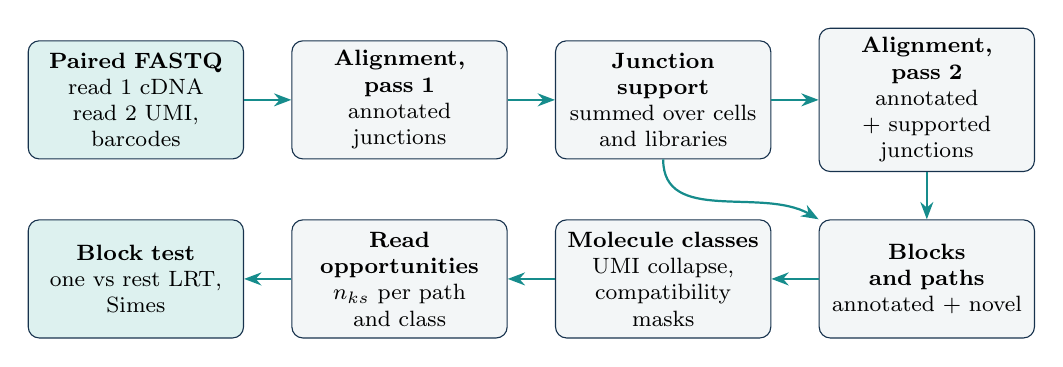
\begin{tikzpicture}[
  stage/.style={draw=tealeafNavy,rounded corners,fill=tealeafLight,align=center,font=\footnotesize,text width=25mm,minimum height=15mm},
  flow/.style={-{Stealth[length=2.2mm]},thick,draw=tealeafTeal},
  node distance=6mm and 6mm]
\node[stage,fill=tealeafLightTeal] (fastq) {\textbf{Paired FASTQ}\\read 1 cDNA\\read 2 UMI, barcodes};
\node[stage,right=of fastq] (pass1) {\textbf{Alignment, pass 1}\\annotated junctions};
\node[stage,right=of pass1] (junc) {\textbf{Junction support}\\summed over cells\\and libraries};
\node[stage,right=of junc] (pass2) {\textbf{Alignment, pass 2}\\annotated + supported\\junctions};
\node[stage,below=of pass2] (blocks) {\textbf{Blocks and paths}\\annotated + novel};
\node[stage,left=of blocks] (classes) {\textbf{Molecule classes}\\UMI collapse,\\compatibility masks};
\node[stage,left=of classes] (opps) {\textbf{Read}\\\textbf{opportunities}\\$n_{ks}$ per path and class};
\node[stage,left=of opps,fill=tealeafLightTeal] (test) {\textbf{Block test}\\one vs rest LRT,\\Simes};
\draw[flow] (fastq)--(pass1);
\draw[flow] (pass1)--(junc);
\draw[flow] (junc)--(pass2);
\draw[flow] (pass2)--(blocks);
\draw[flow] (junc.south) to[out=-90,in=150] (blocks.north west);
\draw[flow] (blocks)--(classes);
\draw[flow] (classes)--(opps);
\draw[flow] (opps)--(test);
\end{tikzpicture}
\caption{Tealeaf from reads to block tests. Junction support from the first alignment pass defines the known junctions of the second pass; support from the second pass defines the novel paths. No step before the test uses cell-type labels.}
\label{fig:pipeline}
\end{figure}

\begin{figure}[p]
\centering
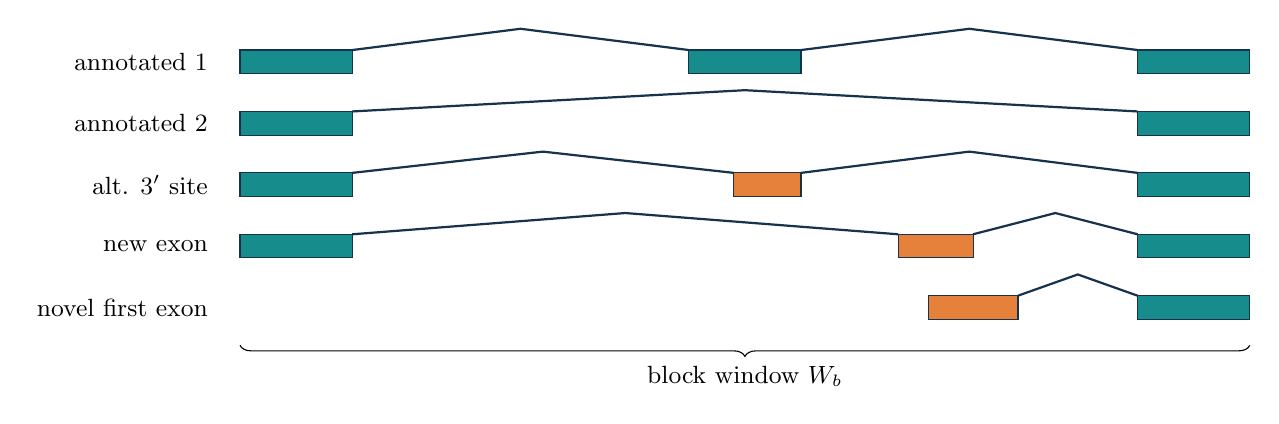
\begin{tikzpicture}[x=0.95mm,y=6mm,
  exon/.style={fill=tealeafTeal,draw=tealeafNavy},
  novel/.style={fill=tealeafOrange,draw=tealeafNavy},
  junction/.style={draw=tealeafNavy,thick}]
\def\pathlabel#1#2{\node[anchor=east,font=\small] at (-3,#1) {#2};}
% annotated paths
\pathlabel{0}{annotated 1}
\draw[exon] (0,-0.25) rectangle (15,0.25); \draw[exon] (60,-0.25) rectangle (75,0.25); \draw[exon] (120,-0.25) rectangle (135,0.25);
\draw[junction] (15,0.25) -- (37.5,0.7) -- (60,0.25); \draw[junction] (75,0.25) -- (97.5,0.7) -- (120,0.25);
\pathlabel{-1.3}{annotated 2}
\draw[exon] (0,-1.55) rectangle (15,-1.05); \draw[exon] (120,-1.55) rectangle (135,-1.05);
\draw[junction] (15,-1.05) -- (67.5,-0.6) -- (120,-1.05);
% alternative acceptor
\pathlabel{-2.6}{alt. 3$'$ site}
\draw[exon] (0,-2.85) rectangle (15,-2.35); \draw[novel] (66,-2.85) rectangle (75,-2.35); \draw[exon] (120,-2.85) rectangle (135,-2.35);
\draw[junction] (15,-2.35) -- (40.5,-1.9) -- (66,-2.35); \draw[junction] (75,-2.35) -- (97.5,-1.9) -- (120,-2.35);
% new exon
\pathlabel{-3.9}{new exon}
\draw[exon] (0,-4.15) rectangle (15,-3.65); \draw[novel] (88,-4.15) rectangle (98,-3.65); \draw[exon] (120,-4.15) rectangle (135,-3.65);
\draw[junction] (15,-3.65) -- (51.5,-3.2) -- (88,-3.65); \draw[junction] (98,-3.65) -- (109,-3.2) -- (120,-3.65);
% novel first exon
\pathlabel{-5.2}{novel first exon}
\draw[novel] (92,-5.45) rectangle (104,-4.95); \draw[exon] (120,-5.45) rectangle (135,-4.95);
\draw[junction] (104,-4.95) -- (112,-4.5) -- (120,-4.95);
% window
\draw[decorate,decoration={brace,mirror,amplitude=4pt}] (0,-6) -- (135,-6) node[midway,below=4pt,font=\small] {block window $W_b$};
\end{tikzpicture}
\caption{Novel paths in a block with two annotated paths (teal). Orange exons are created from novel junctions, an alternative acceptor in an existing exon, a new exon from a pair of novel junctions, and a novel first exon of length $T$ from a donor deep in an intron (more than 300 bases from any exon) whose junction pairs with no other.}
\label{fig:novel}
\end{figure}

\begin{figure}[p]
\centering
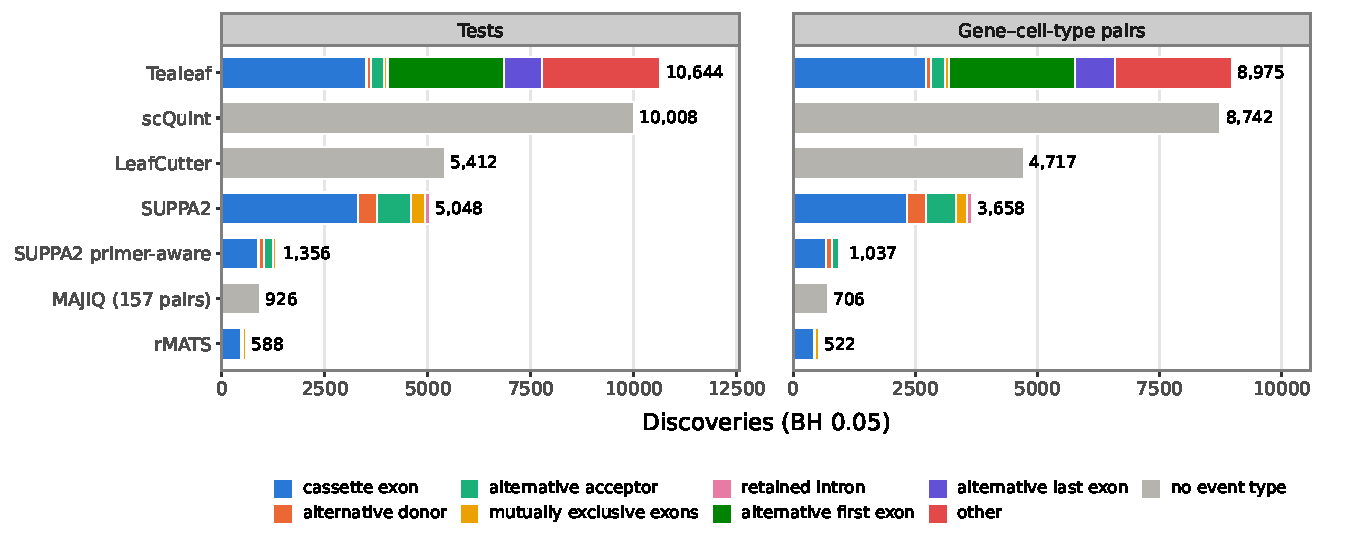
\includegraphics[width=\textwidth]{figures/discoveries_by_event_all.pdf}
\caption{Full-data discoveries as in Fig.~\ref{fig:brain}d, on all 190 cell-type pairs each method tests; methods tested on fewer pairs give their number of pairs.}
\label{fig:discoveries-all}
\end{figure}

\begin{figure}[p]
\centering
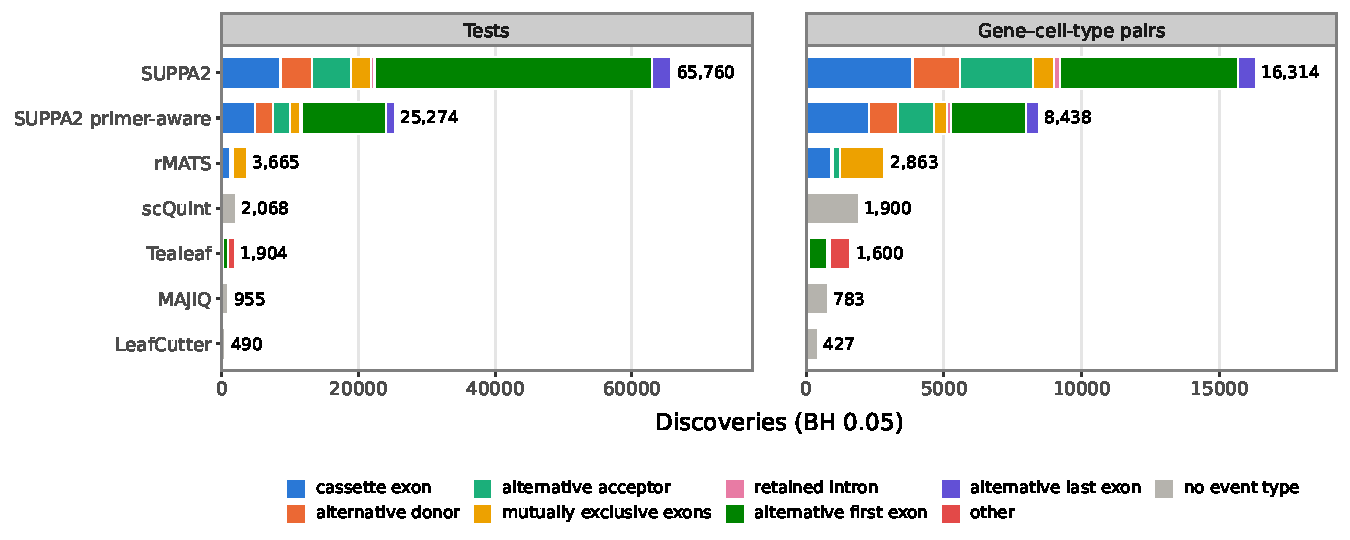
\includegraphics[width=\textwidth]{figures/discoveries_by_event_GSE320507.pdf}
\caption{GSE320507 full-data discoveries (BH 0.05 within method) on the 135 cell-type pairs tested by every method, counted as tests (left) and as gene--cell-type pairs with at least one discovery (right), by event class, as in Fig.~\ref{fig:brain}d. Tests called by the coverage-only null are removed for every method except SUPPA2.}
\label{fig:discoveries-pbmc}
\end{figure}

\begin{figure}[p]
\centering
\panel{a}\\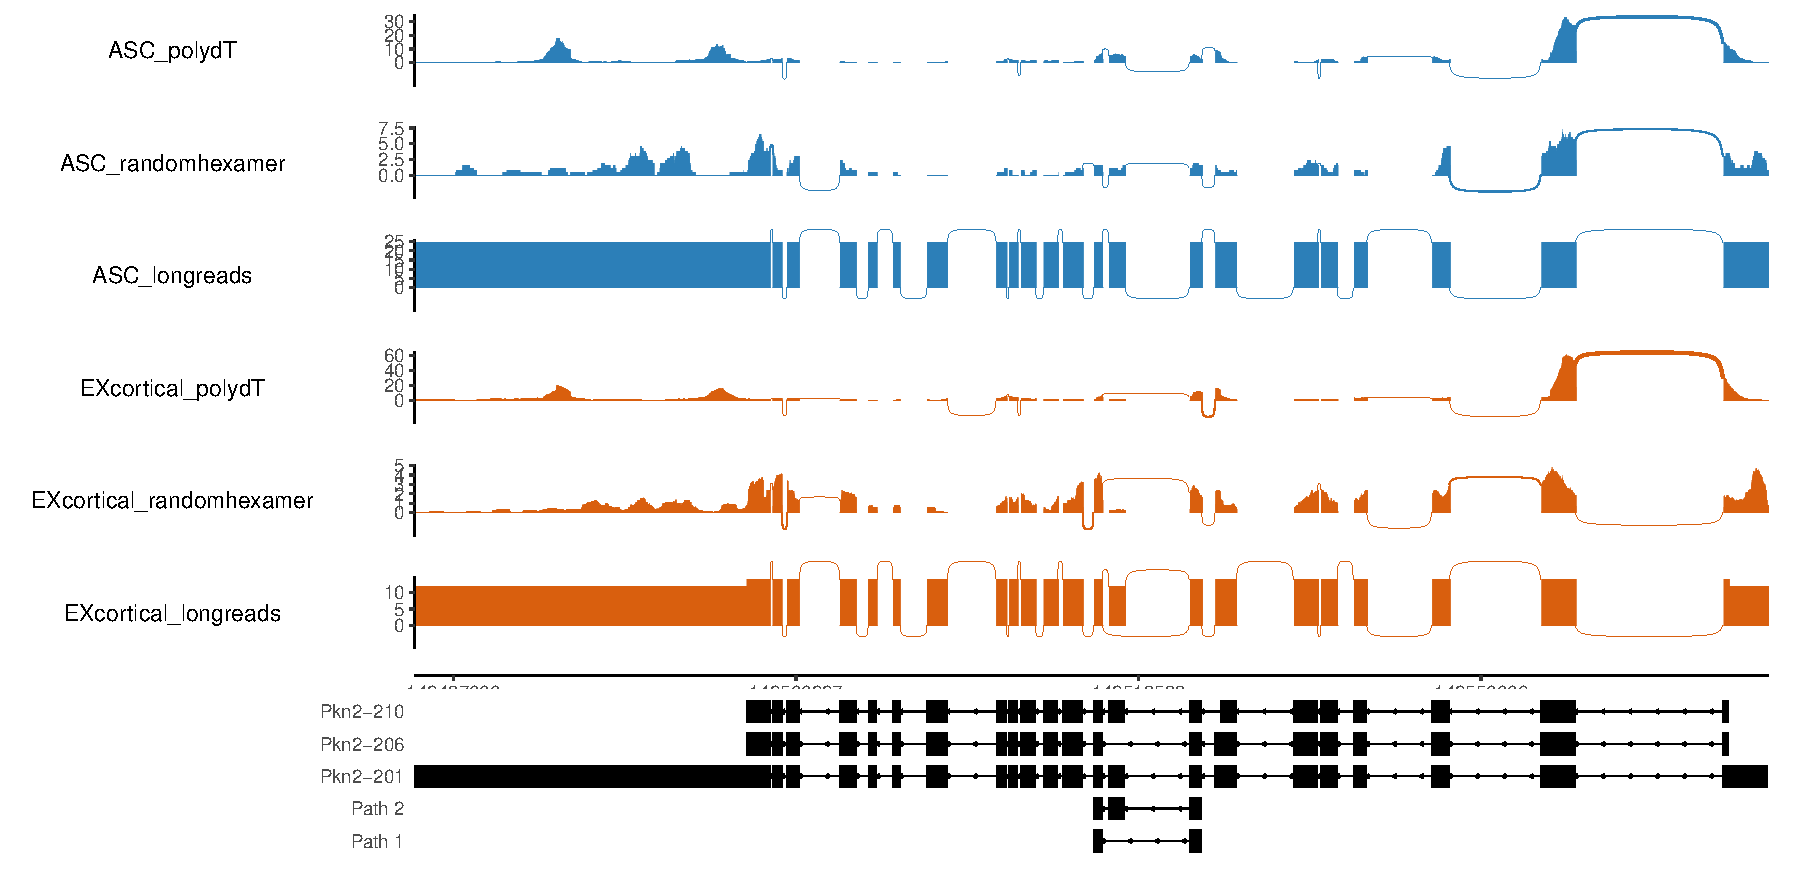
\includegraphics[width=0.95\textwidth,height=0.28\textheight,keepaspectratio]{figures/sashimi_Pkn2_B3_gene.pdf}\\[4pt]
\panel{b}\\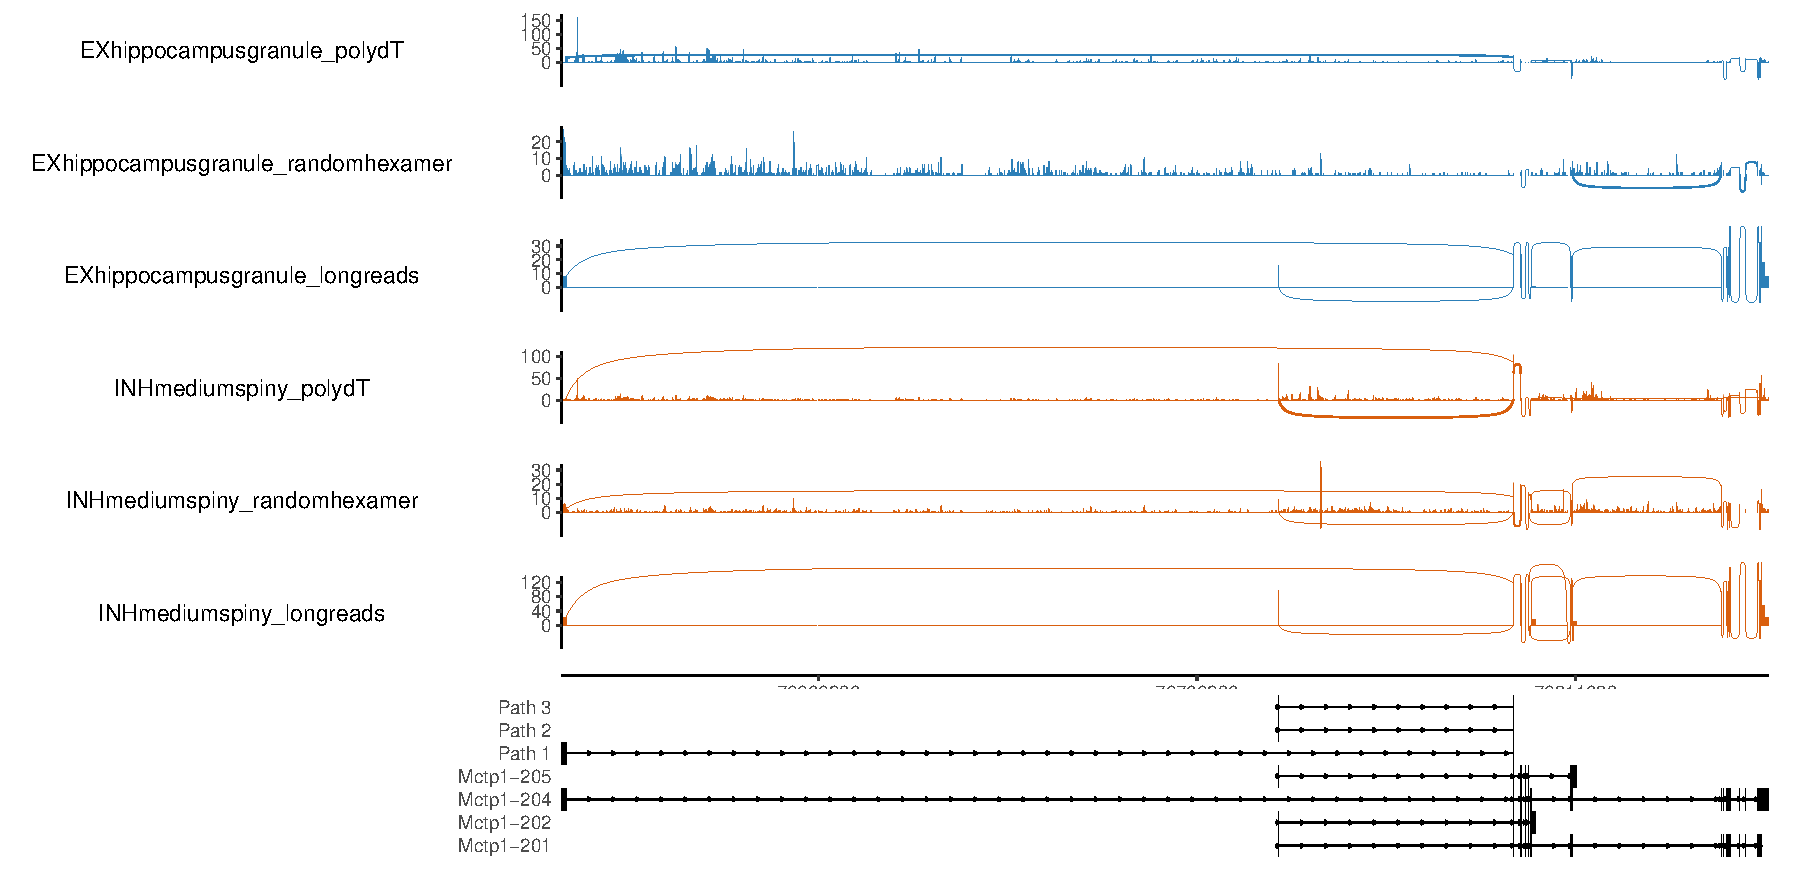
\includegraphics[width=0.95\textwidth,height=0.28\textheight,keepaspectratio]{figures/sashimi_Mctp1_B1_gene.pdf}\\[4pt]
\panel{c}\\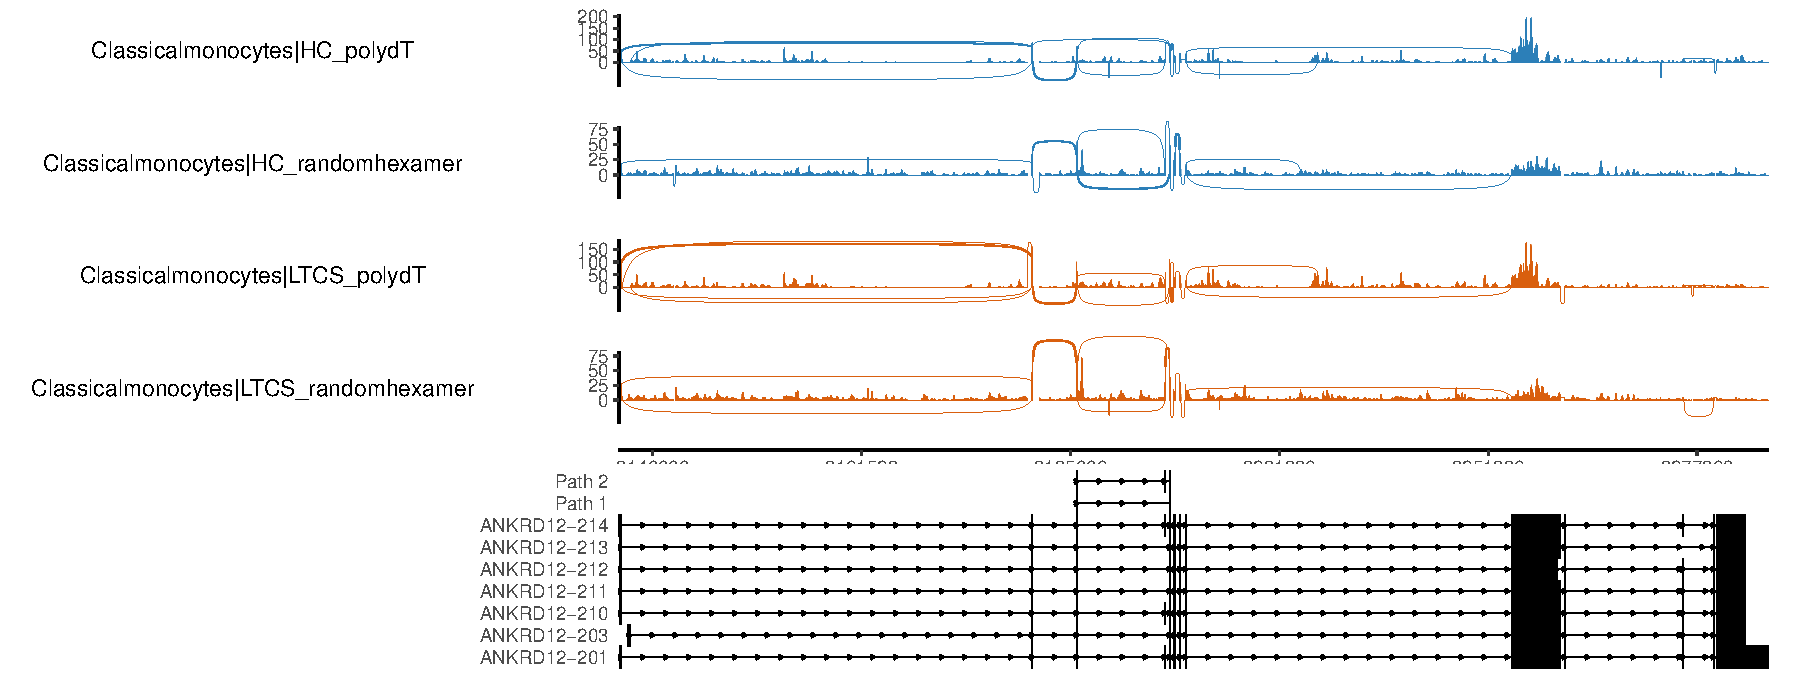
\includegraphics[width=0.95\textwidth,height=0.28\textheight,keepaspectratio]{figures/sashimi_ltcs_ANKRD12_B2_gene.pdf}
\caption{Whole-gene sashimi views of the examples of Figs.~\ref{fig:examples} and \ref{fig:blood}: \textbf{a}, \emph{Pkn2}; \textbf{b}, \emph{Mctp1}; \textbf{c}, \emph{ANKRD12}. Tracks as in the block views; junction labels are omitted, and the block's paths mark the block.}
\label{fig:gene-views}
\end{figure}

\begin{figure}[p]
\centering
\makebox[\textwidth][c]{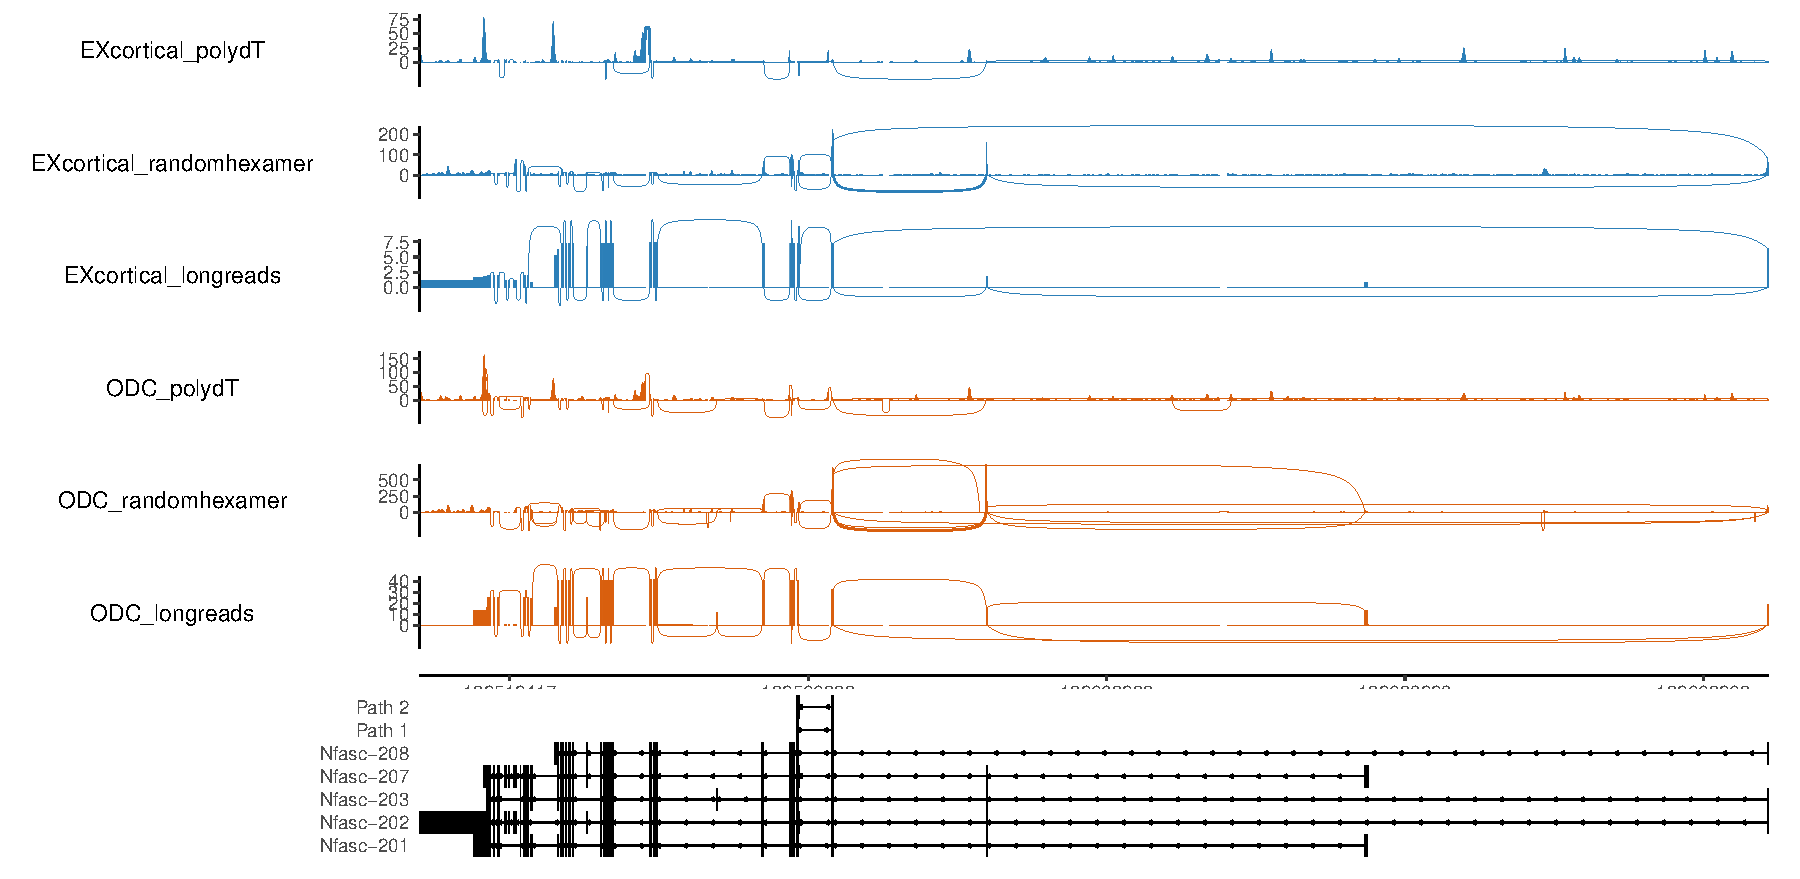
\includegraphics[width=1.15\textwidth,height=0.4\textheight,keepaspectratio]{figures/sashimi_Nfasc_B2_gene.pdf}}\\
(a)\\[4pt]
\makebox[\textwidth][c]{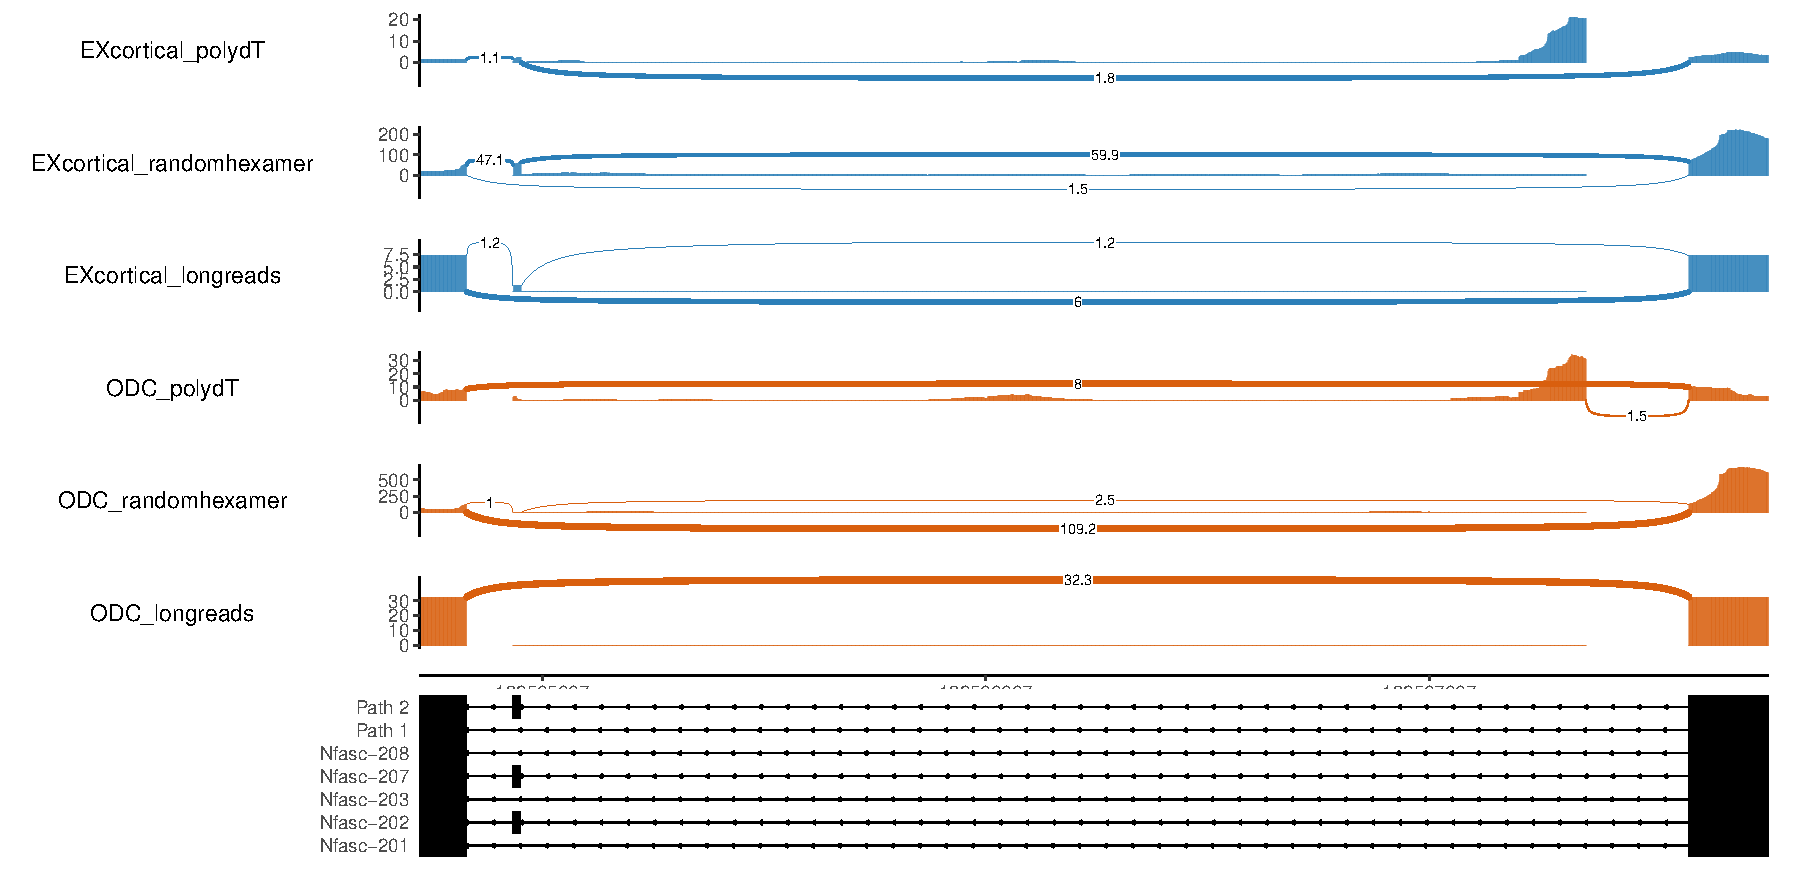
\includegraphics[width=1.15\textwidth,height=0.4\textheight,keepaspectratio]{figures/sashimi_Nfasc_B2.pdf}}\\
(b)
\caption{Nfasc block 2, cortical excitatory neurons against oligodendrocytes. Panels as in Fig.~\ref{fig:examples}a, with the whole gene in (a).}
\label{fig:nfasc}
\end{figure}

\begin{figure}[p]
\centering
\makebox[\textwidth][c]{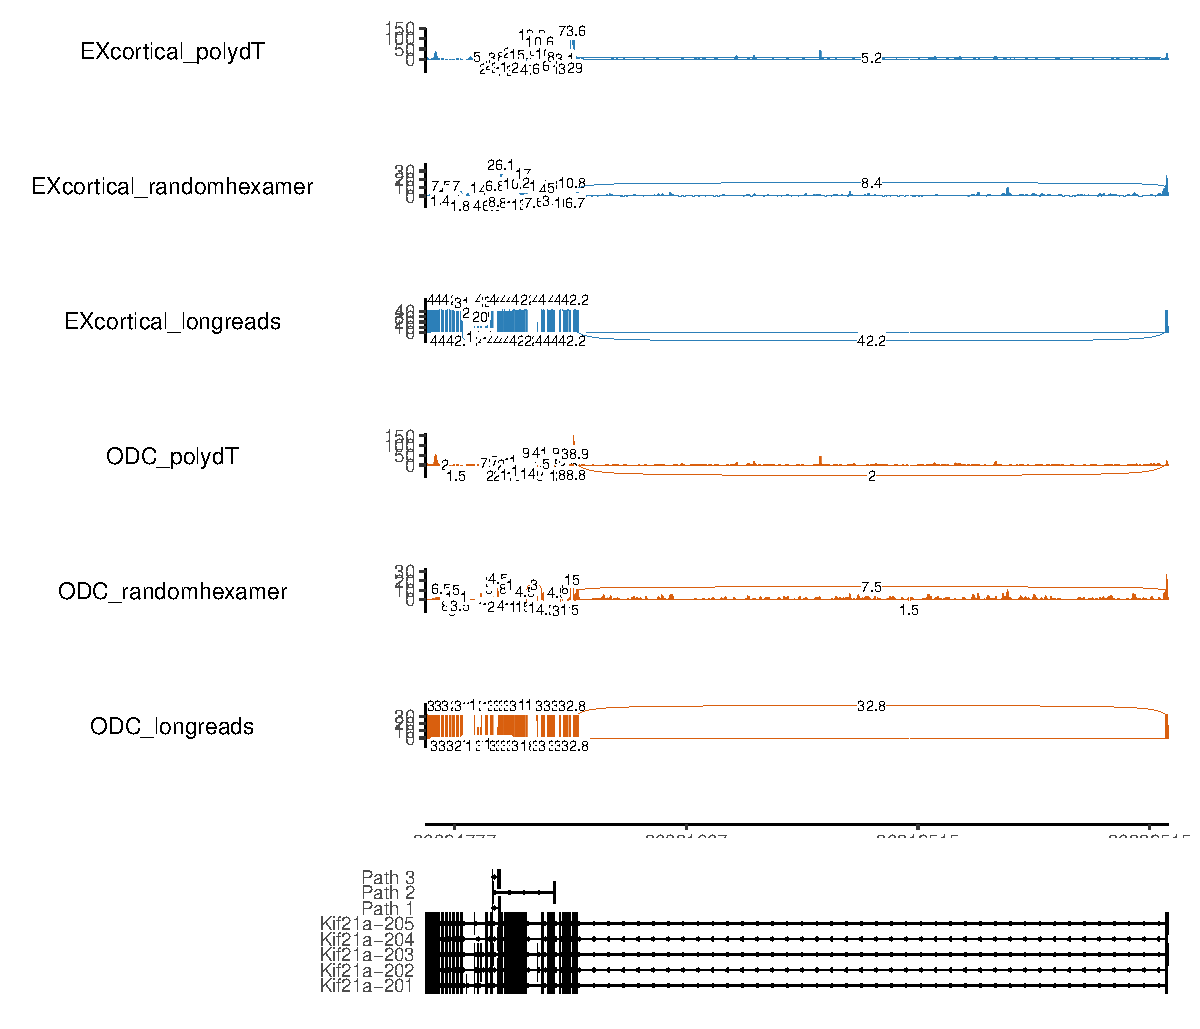
\includegraphics[width=1.15\textwidth,height=0.4\textheight,keepaspectratio]{figures/sashimi_Kif21a_B3_gene.pdf}}\\
(a)\\[4pt]
\makebox[\textwidth][c]{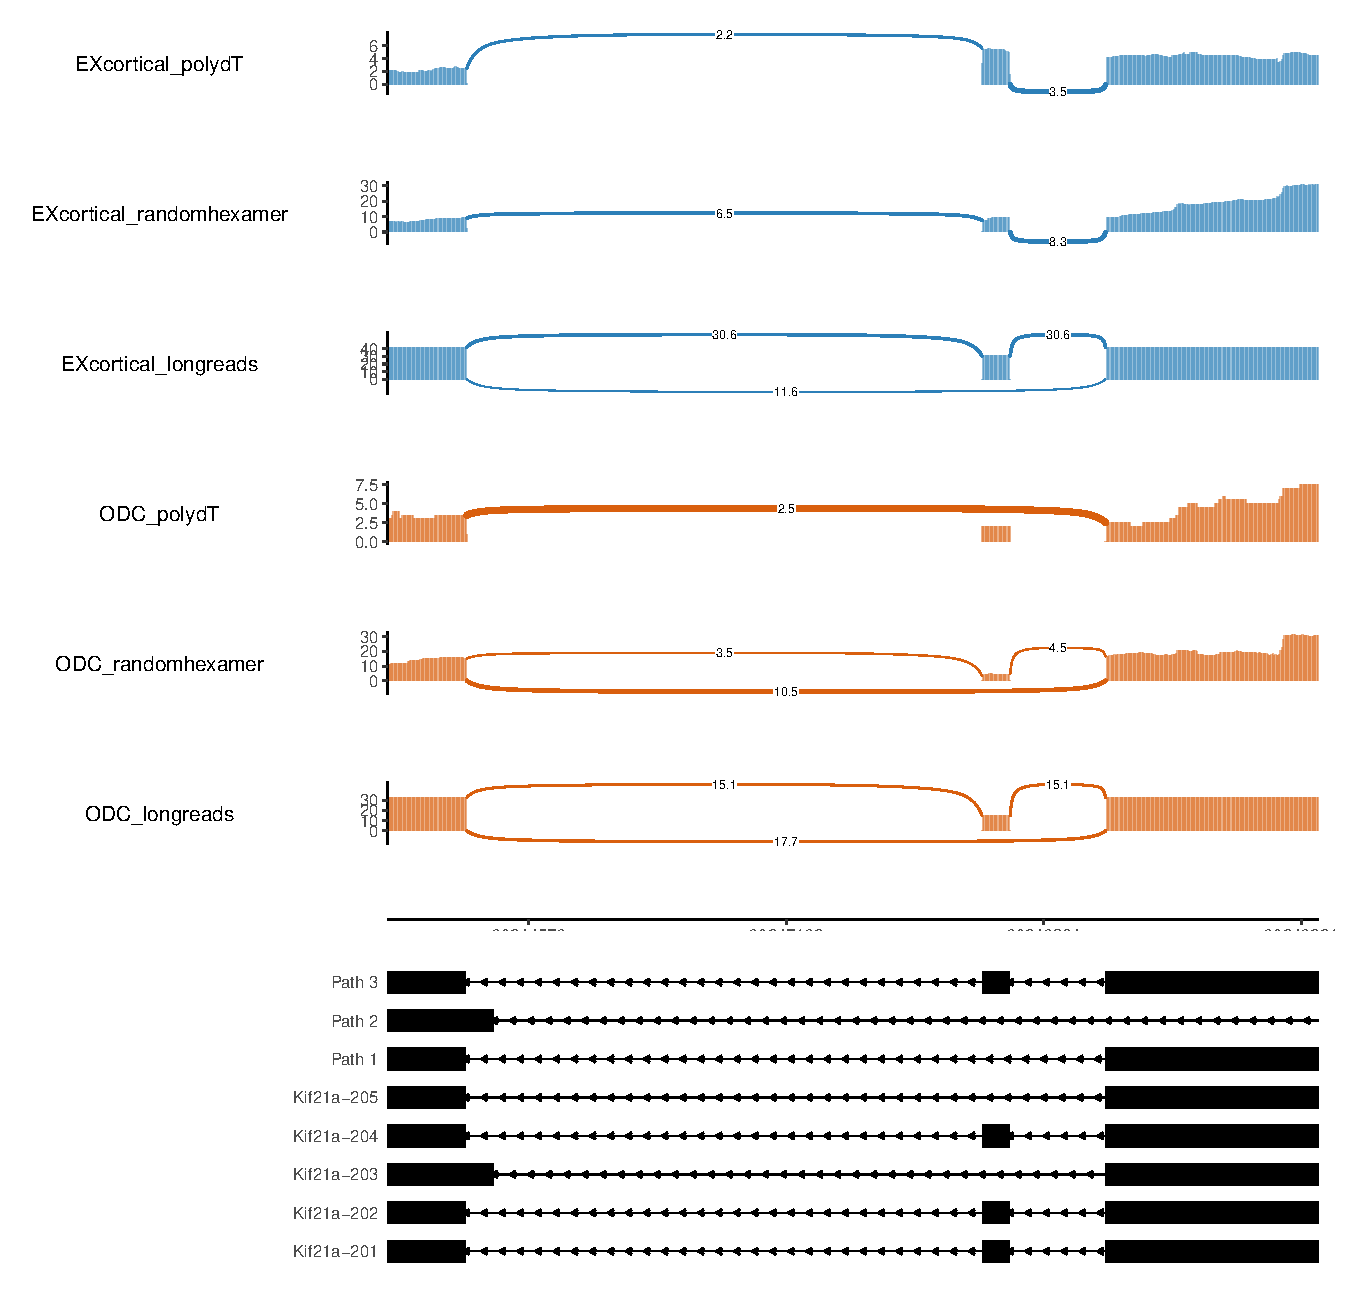
\includegraphics[width=1.15\textwidth,height=0.4\textheight,keepaspectratio]{figures/sashimi_Kif21a_B3.pdf}}\\
(b)
\caption{Kif21a block 3, cortical excitatory neurons against oligodendrocytes. Panels as in Fig.~\ref{fig:examples}a, with the whole gene in (a).}
\label{fig:kif21a}
\end{figure}

\begin{figure}[p]
\centering
\begin{minipage}[t]{0.49\textwidth}\centering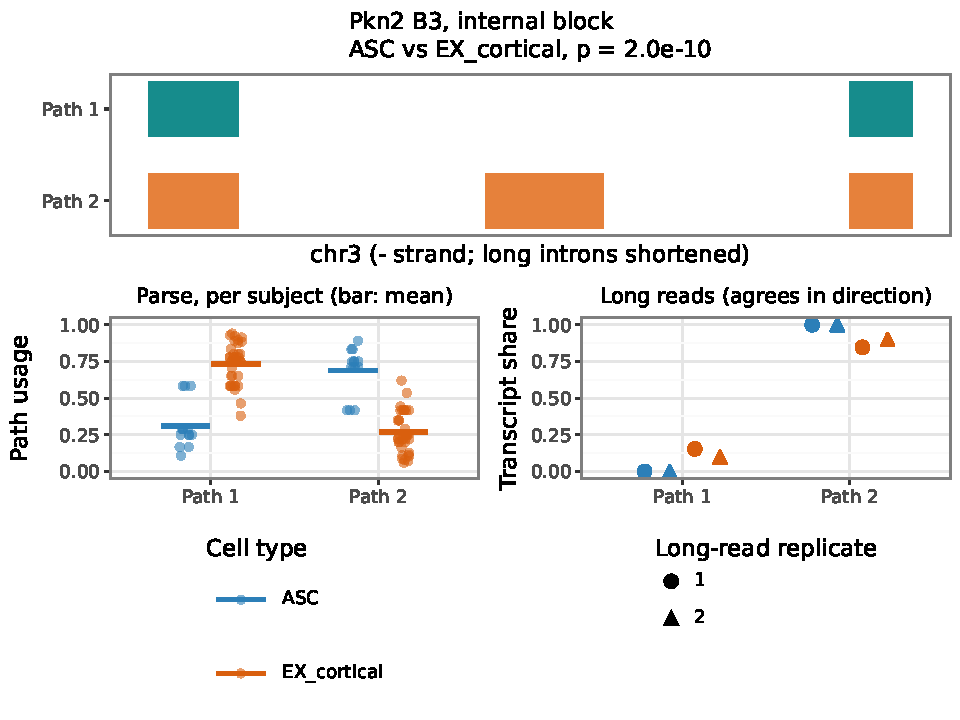
\includegraphics[width=\textwidth]{figures/example_Pkn2_B3.pdf}\\(a)\end{minipage}\hfill
\begin{minipage}[t]{0.49\textwidth}\centering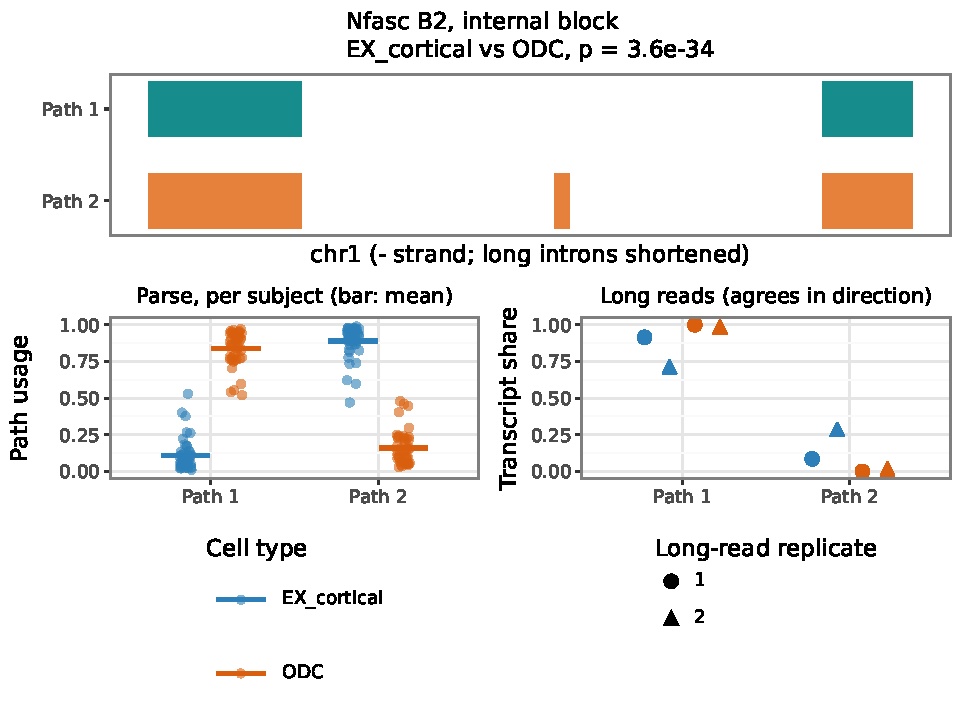
\includegraphics[width=\textwidth]{figures/example_Nfasc_B2.pdf}\\(b)\end{minipage}\\[6pt]
\begin{minipage}[t]{0.49\textwidth}\centering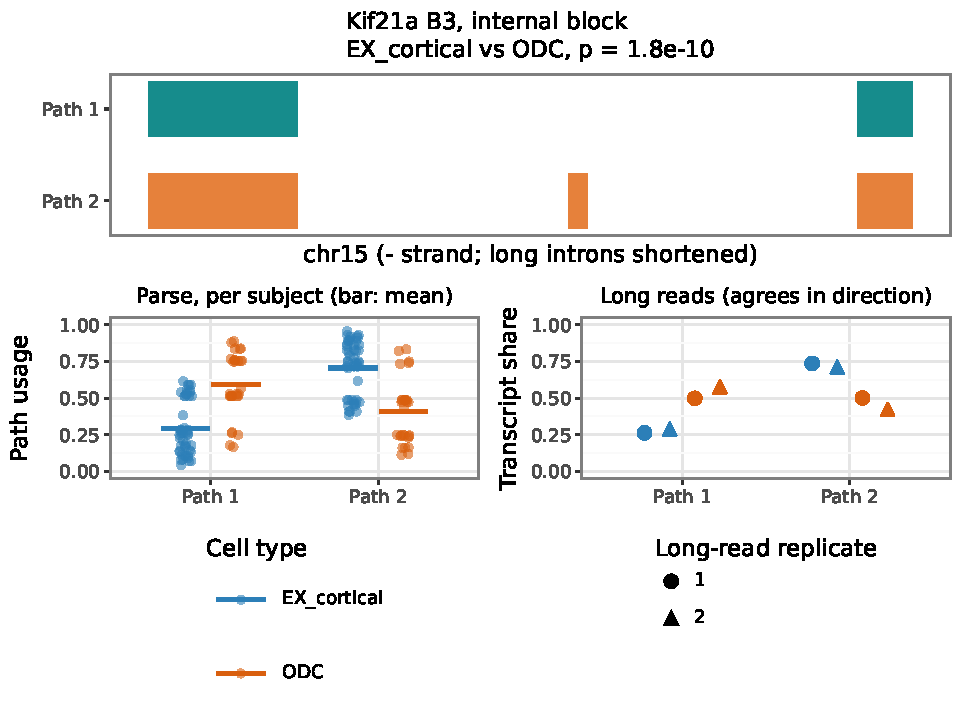
\includegraphics[width=\textwidth]{figures/example_Kif21a_B3.pdf}\\(c)\end{minipage}\hfill
\begin{minipage}[t]{0.49\textwidth}\centering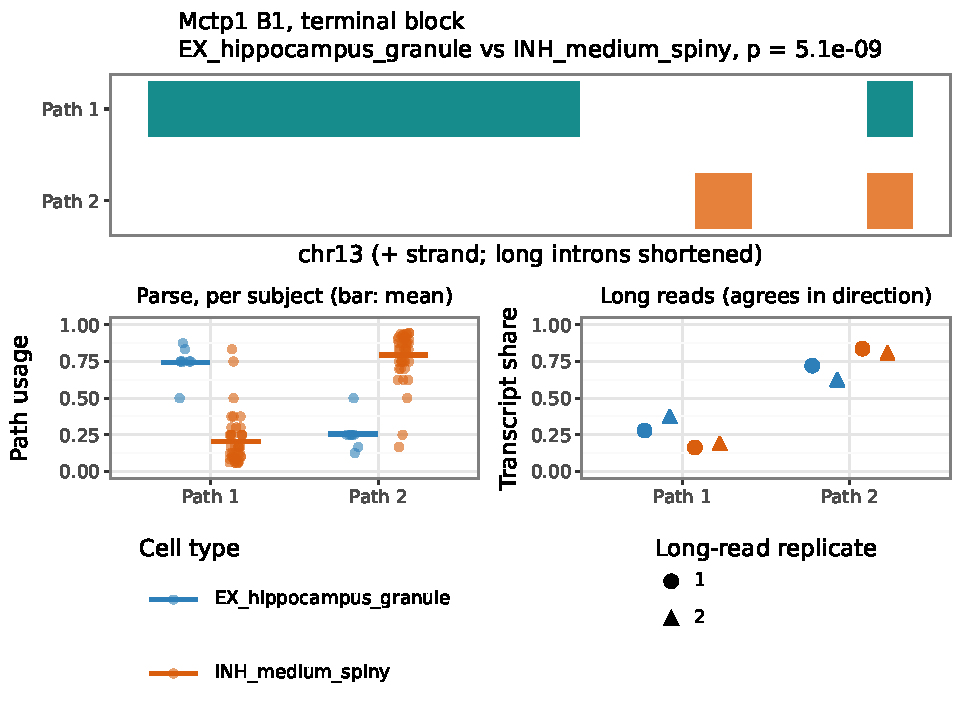
\includegraphics[width=\textwidth]{figures/example_Mctp1_B1.pdf}\\(d)\end{minipage}\\[6pt]
\caption{Path usage in the four examples: (a) Pkn2, (b) Nfasc, (c) Kif21a, (d) Mctp1. In each panel, top, the tested paths, numbered as in the sashimi plots (introns longer than 300 bases shortened; merged paths are drawn by their first member); bottom left, the path usage of each subject in the Parse data with the mean over subjects (bars); bottom right, the transcript share of each path in the two long-read replicates.}
\label{fig:usage}
\end{figure}

\begin{figure}[p]
\centering
\makebox[\textwidth][c]{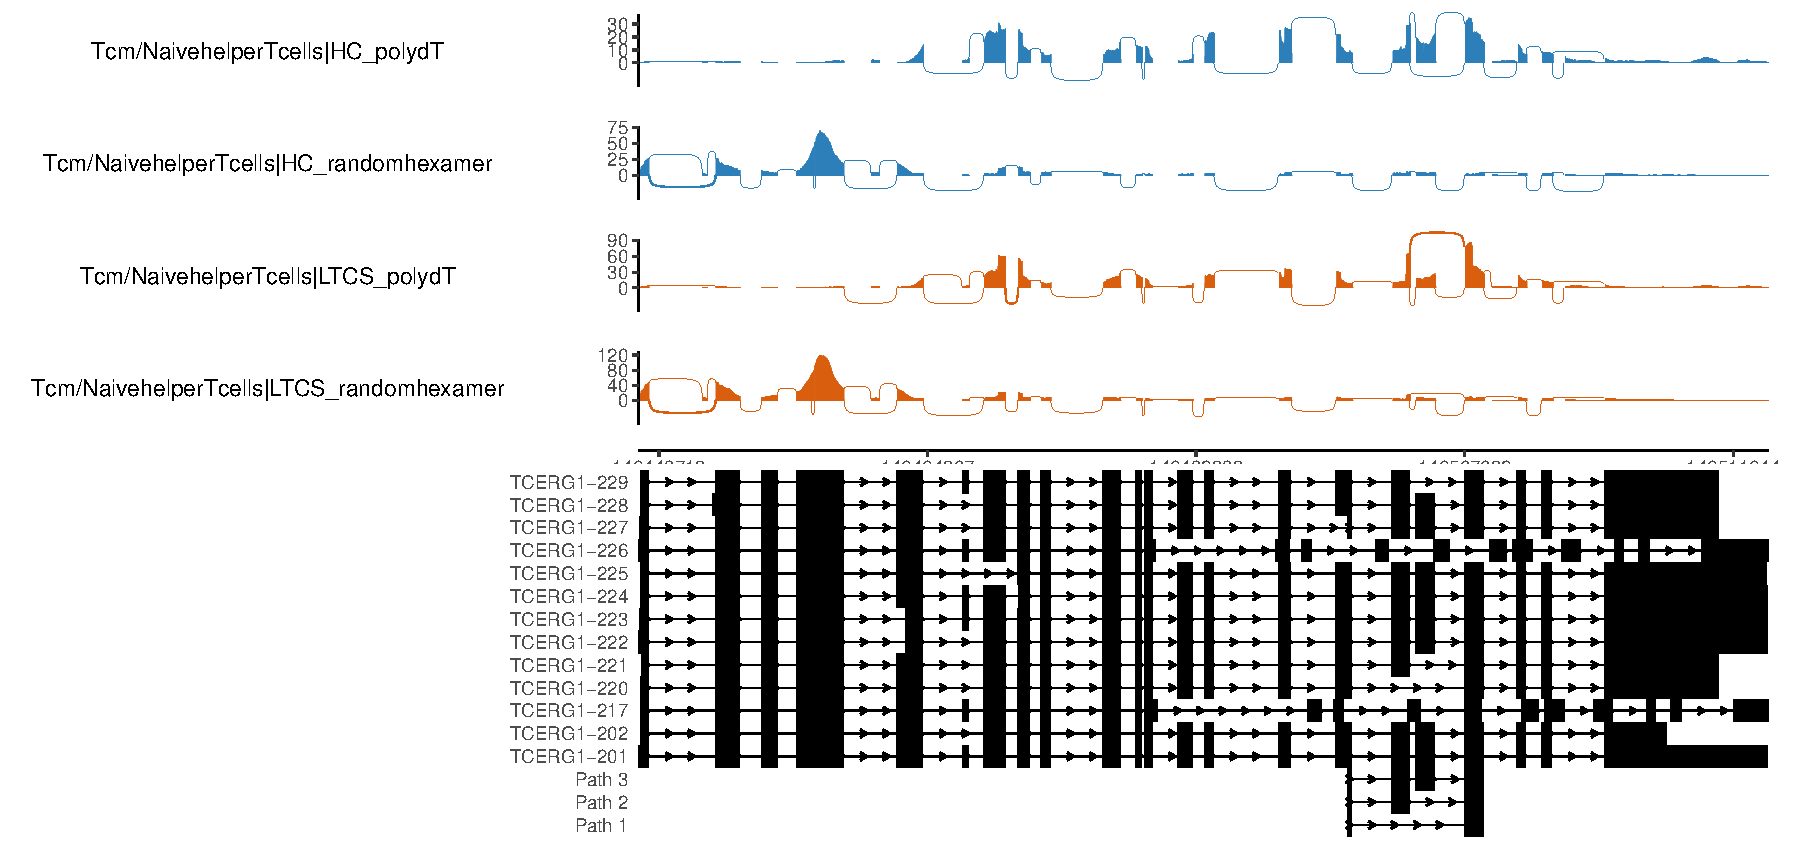
\includegraphics[width=1.15\textwidth,height=0.4\textheight,keepaspectratio]{figures/sashimi_ltcs_TCERG1_B7_gene.pdf}}\\
(a)\\[4pt]
\makebox[\textwidth][c]{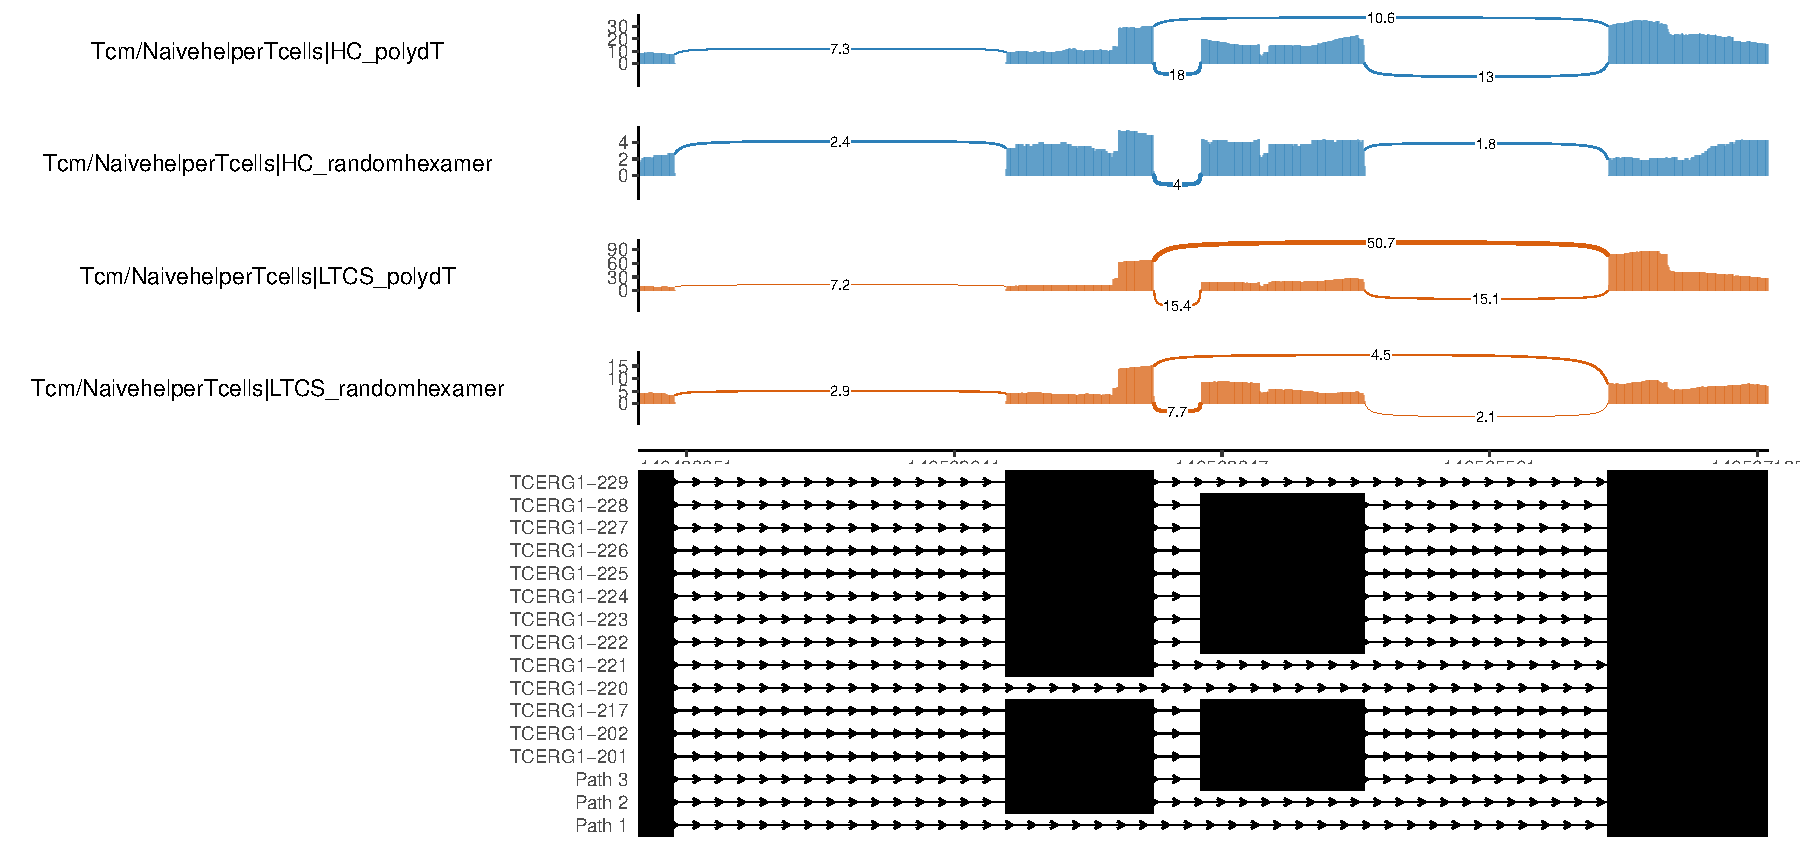
\includegraphics[width=1.15\textwidth,height=0.4\textheight,keepaspectratio]{figures/sashimi_ltcs_TCERG1_B7.pdf}}\\
(b)
\caption{TCERG1 block 7 in naive and central-memory helper T cells, HC against LTCS donors. Panels as in Fig.~\ref{fig:blood}e, with the whole gene in (a).}
\label{fig:tcerg1}
\end{figure}
\begin{figure}[p]
\centering
\makebox[\textwidth][c]{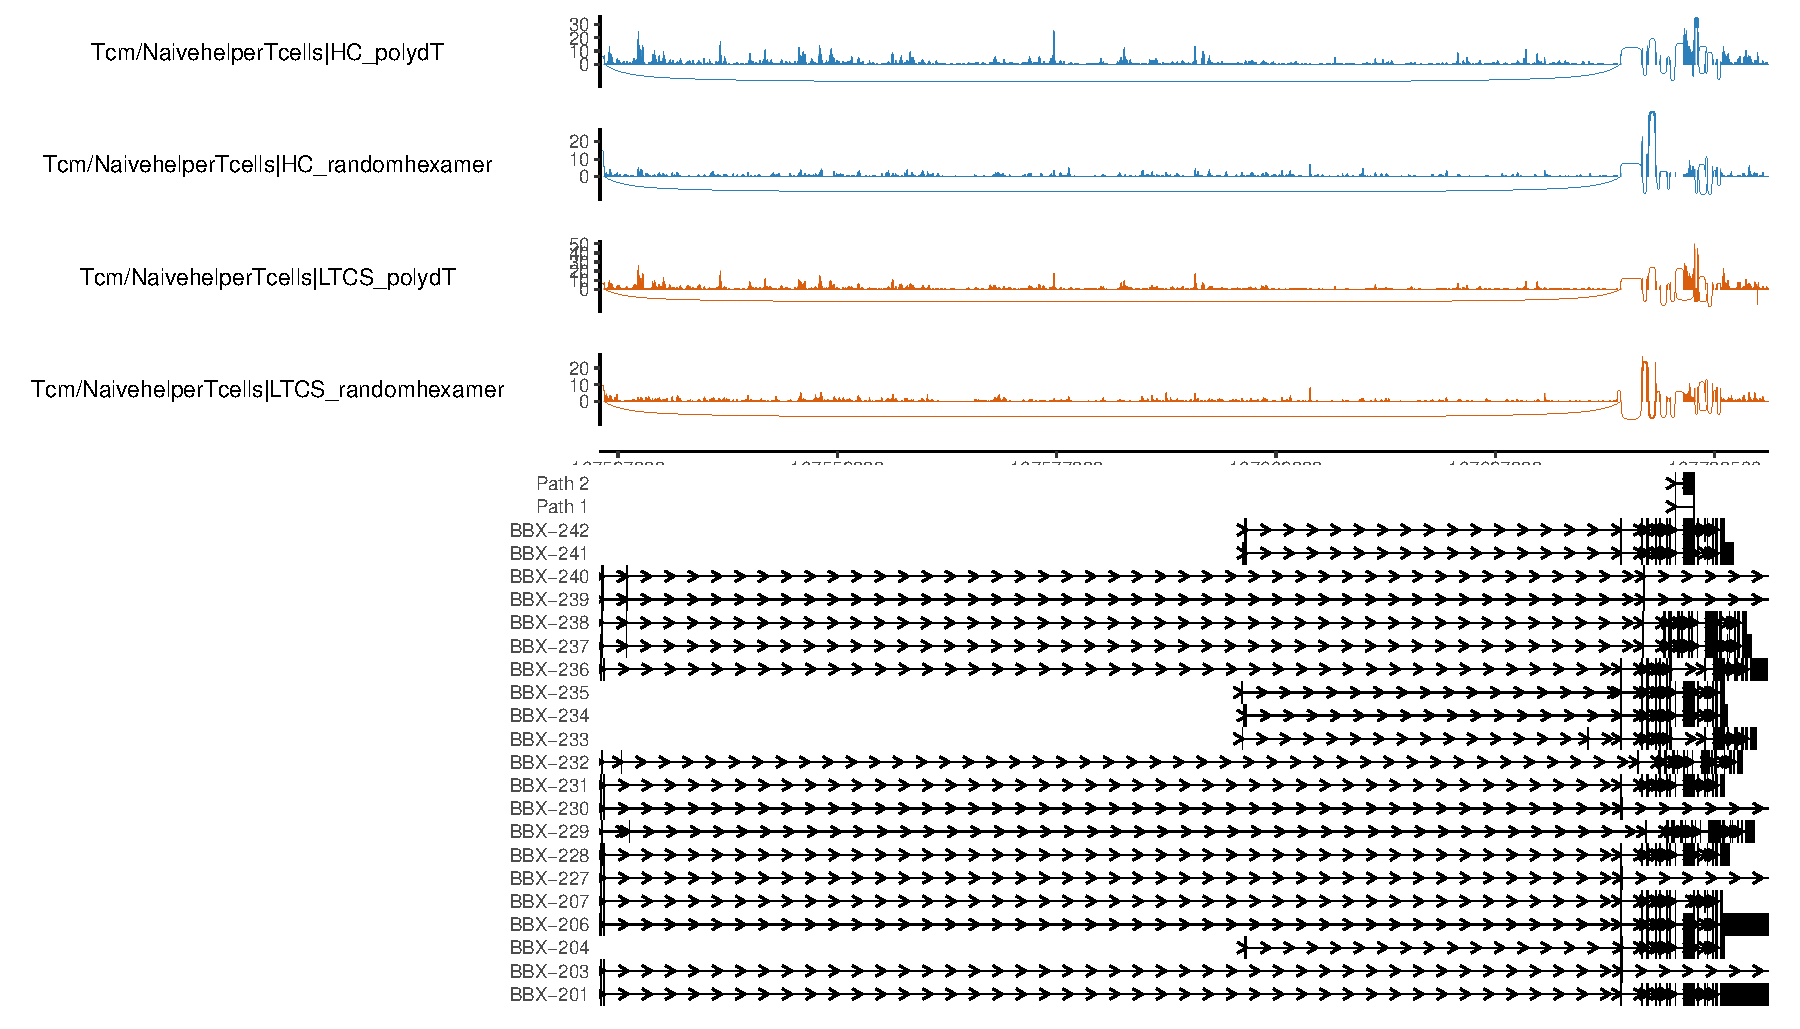
\includegraphics[width=1.15\textwidth,height=0.4\textheight,keepaspectratio]{figures/sashimi_ltcs_BBX_B4_gene.pdf}}\\
(a)\\[4pt]
\makebox[\textwidth][c]{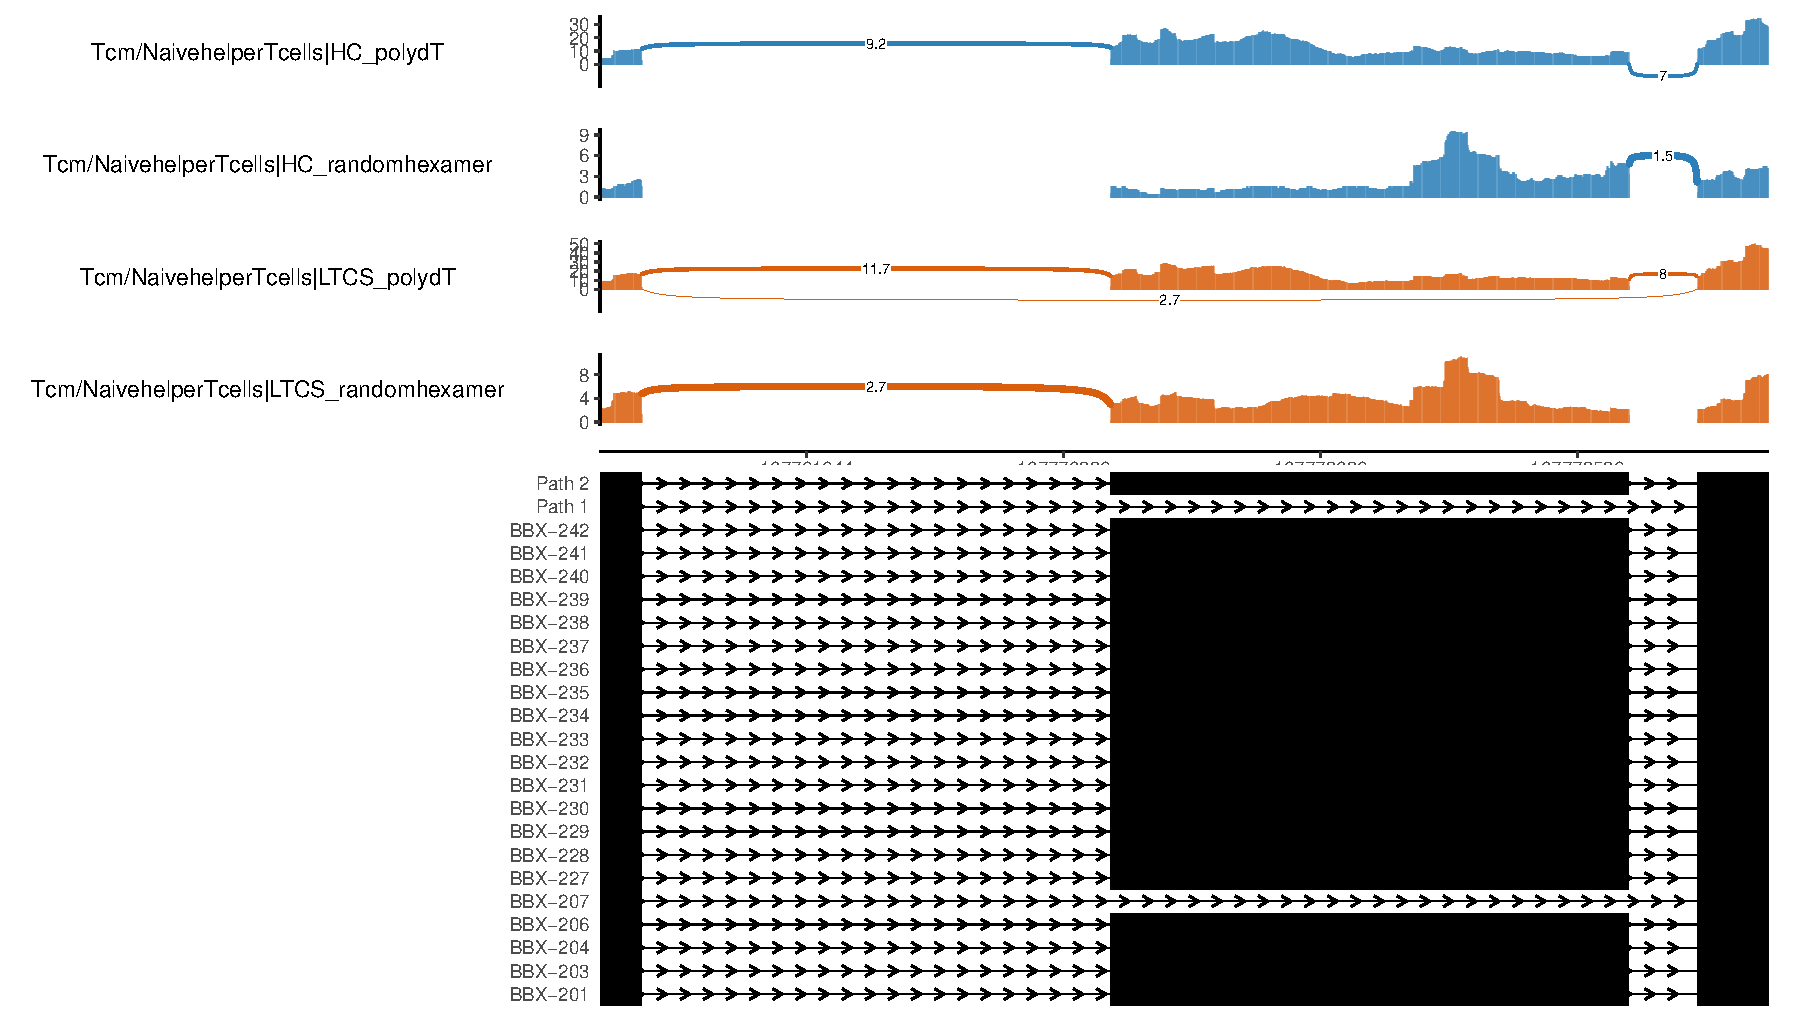
\includegraphics[width=1.15\textwidth,height=0.4\textheight,keepaspectratio]{figures/sashimi_ltcs_BBX_B4.pdf}}\\
(b)
\caption{BBX block 4 in naive and central-memory helper T cells, HC against LTCS donors. Panels as in Fig.~\ref{fig:blood}e, with the whole gene in (a).}
\label{fig:bbx}
\end{figure}
\begin{figure}[p]
\centering
\makebox[\textwidth][c]{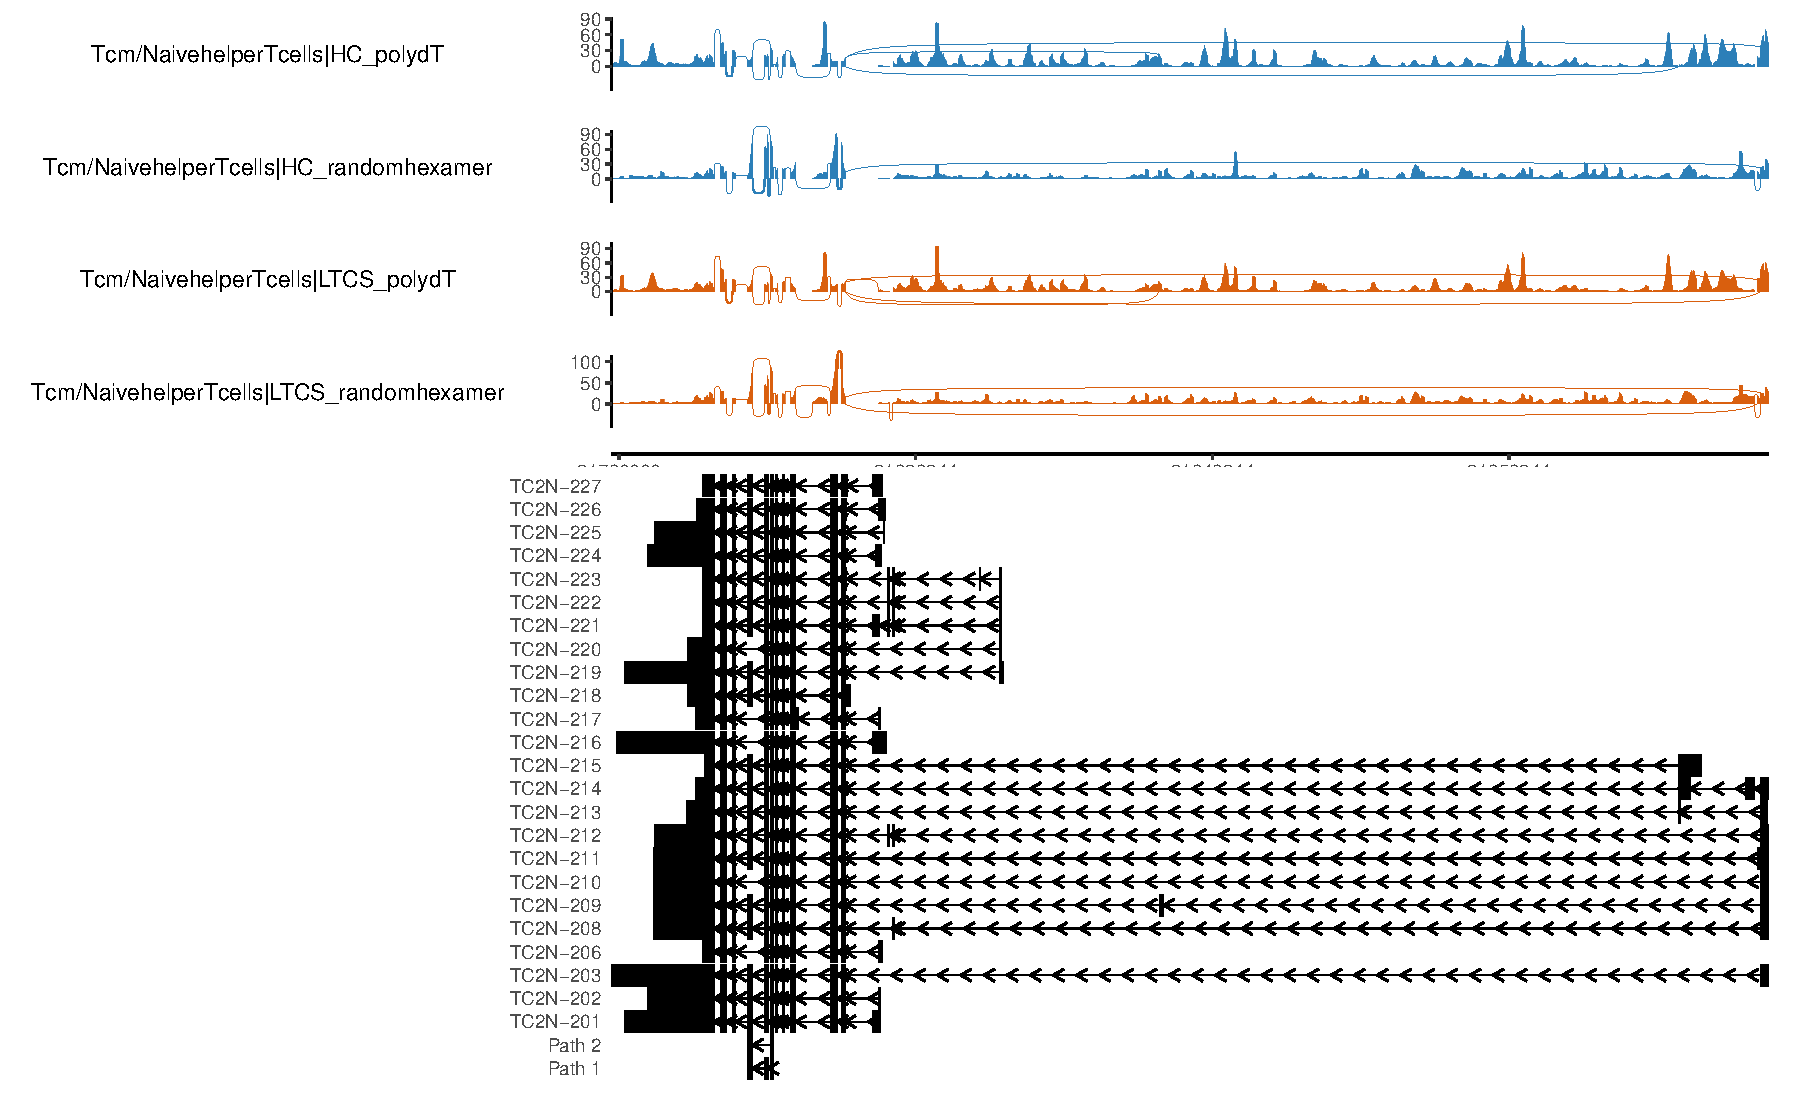
\includegraphics[width=1.15\textwidth,height=0.4\textheight,keepaspectratio]{figures/sashimi_ltcs_TC2N_N3_gene.pdf}}\\
(a)\\[4pt]
\makebox[\textwidth][c]{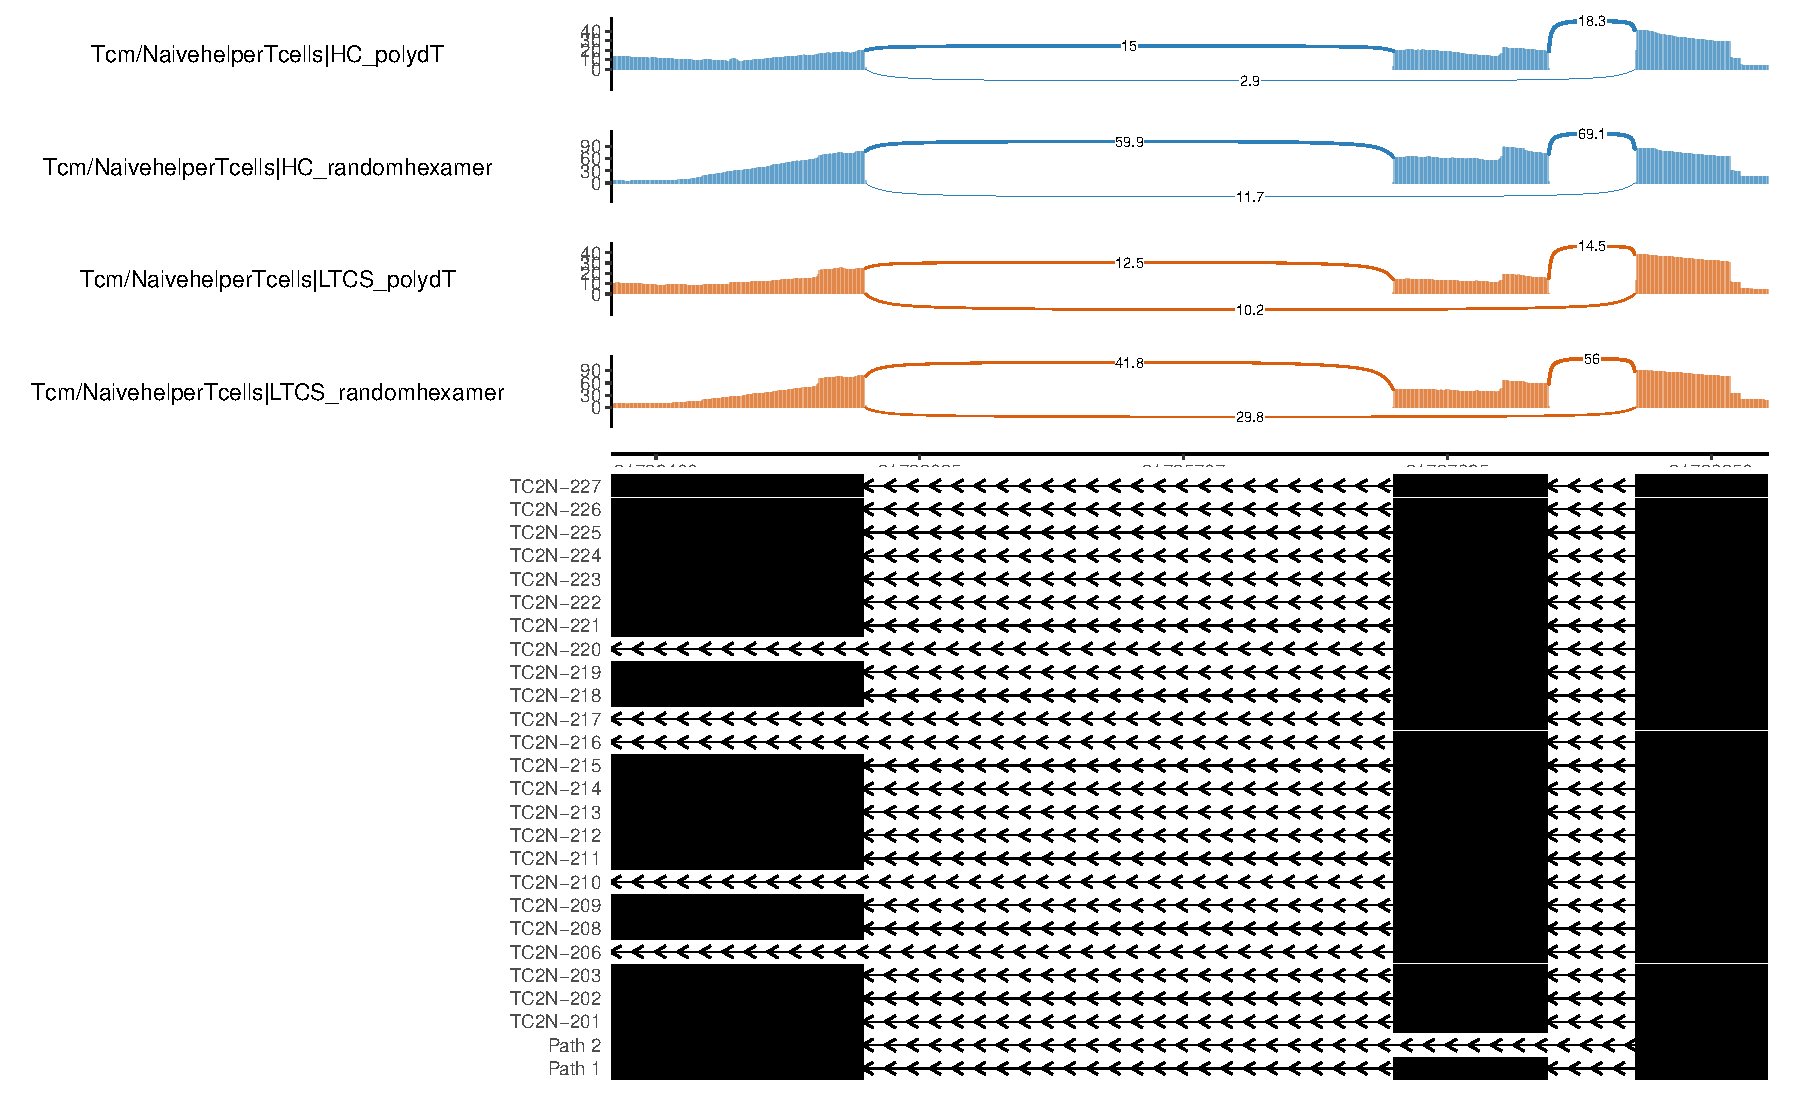
\includegraphics[width=1.15\textwidth,height=0.4\textheight,keepaspectratio]{figures/sashimi_ltcs_TC2N_N3.pdf}}\\
(b)
\caption{TC2N novel block 3 in naive and central-memory helper T cells, HC against LTCS donors. Panels as in Fig.~\ref{fig:blood}e, with the whole gene in (a).}
\label{fig:tc2n}
\end{figure}

\clearpage
\subsection*{Supplementary Tables}

\begin{table}[ht]
\centering
\small
\setlength{\tabcolsep}{4pt}
\begin{tabular}{lcccccc}
\toprule
 & LeafCutter & MAJIQ & SUPPA2 & SUPPA2-PA & rMATS & scQuint\\
\midrule
\multicolumn{7}{l}{\emph{Matched universe}}\\
Genes & 263 & 2{,}758 & 3{,}411 & 3{,}072 & 5{,}070 & 3{,}603\\
Tealeaf replicated & 63 & 201 & 124 & 130 & 158 & 179\\
Comparator replicated & 35 & 17 & 8 & 0 & 4 & 134\\
\midrule
\multicolumn{7}{l}{\emph{Comparator universe}}\\
Genes & 279 & 2{,}996 & 5{,}068 & 3{,}901 & 6{,}838 & 4{,}220\\
Tealeaf replicated & 63 & 196 & 101 & 115 & 136 & 172\\
Comparator replicated & 36 & 15 & 0 & 0 & 4 & 123\\
\midrule
Comparator $A_{100}$ & .918 & .944 & .870 & .625 & .898 & .912\\
\bottomrule
\end{tabular}
\caption{Replicated genes on each comparator's matched and comparator universes, and long-read direction. SUPPA2-PA is primer-aware SUPPA2. Tests called by the coverage-only null are removed for Tealeaf and every comparator except SUPPA2 and SUPPA2-PA (Section~\ref{sec:coverage-null}, which also gives the results without removal). Tealeaf has $A_{100}=0.946$ (95 of its 100 top-ranked evaluable tests agree with long reads; $A_{40}=0.963$, $A_{200}=0.942$).}
\label{tab:results}
\end{table}

\begin{table}[ht]
\centering
\footnotesize
\setlength{\tabcolsep}{4pt}
\begin{tabular}{lrrrrr}
\toprule
Event class & Tests & Discoveries & Novel path & LR agreement & Top 100\\
\midrule
cassette exon & 217{,}758 & 3{,}553 & 1{,}555 & 0.88 (449) & 36/37\\
alternative first exon & 101{,}666 & 2{,}840 & 2{,}207 & 0.89 (142) & 22/22\\
compound internal & 104{,}884 & 1{,}635 & 1{,}229 & 0.84 (77) & 1/1\\
alternative last exon & 57{,}878 & 941 & 648 & 0.86 (76) & 21/25\\
alternative first and last exons & 24{,}646 & 883 & 740 & 0.85 (47) & 9/9\\
alternative acceptor & 100{,}863 & 313 & 249 & 0.83 (41) & 2/2\\
alternative transcript end & 9{,}055 & 150 & 31 & 1.00 (11) & 1/1\\
alternative donor & 57{,}294 & 113 & 89 & 0.53 (15) & 0/0\\
multi-exon skipping & 8{,}988 & 99 & 57 & 0.90 (21) & 3/3\\
mutually exclusive exons & 2{,}701 & 82 & 11 & 0.88 (8) & 0/0\\
alternative transcript start & 2{,}994 & 60 & 8 & 0.75 (4) & 0/0\\
complex internal & 4{,}982 & 60 & 58 & 1.00 (3) & 0/0\\
retained intron & 1{,}244 & 13 & 13 & -- (0) & 0/0\\
\bottomrule
\end{tabular}
\caption{Full-data tests by event class. Novel path counts discoveries that retain an unannotated path. LR agreement is the fraction of long-read-evaluable discoveries whose direction agrees with the long reads (number evaluable in parentheses); Top 100 gives agreeing over all tests of the class among the 100 top-ranked long-read-evaluable tests.}
\label{tab:events}
\end{table}

\begin{table}[ht]
\centering
\small
\begin{tabular}{lrrr}
\toprule
 & GSE320507 & GSE327907 & GSE334840\\
\midrule
Donors (per half) & 38 (19) & 12 (6) & 8 (4)\\
Cells & 70{,}643 & 24{,}314 & 23{,}000\\
Cell types & 19 & 10 & 8\\
Read 1 length & 136 & 150 & 66\\
Read pairs (billions) & 1.84 & 11.7 & 2.52\\
\midrule
Full-data tests & 1{,}504{,}546 & 200{,}346 & 80{,}470\\
Discoveries & 2{,}340 & 472 & 15\\
Gene--pair discoveries & 1{,}847 & 377 & 13\\
\midrule
Genes tested in both halves & 10{,}079 & 8{,}640 & 5{,}211\\
Discoveries, half 1 / half 2 & 133 / 96 & 15 / 29 & 0 / 0\\
Replicated genes & 65 & 5 & 0\\
\bottomrule
\end{tabular}
\caption{Cell-type contrasts in three PBMC datasets. Cells are those of the contrasts (unstimulated or control cells for GSE327907 and GSE334840); read pairs are for all cells of the dataset. Discoveries are tests with BH-adjusted $p\le0.05$, and gene--pair discoveries (gene, cell-type pair) keys with Simes-combined adjusted $p\le0.05$. Half discoveries and replicated genes are gene-level, on the genes tested in both halves.}
\label{tab:pbmc}
\end{table}

\begin{table}[ht]
\centering
\small
\begin{tabular}{lrrr}
\toprule
 & GSE320507 & GSE327907 & GSE334840\\
\midrule
Long-read cell types (pairs) & 14 (91) & 7 (20) & 7 (20)\\
Evaluable tests & 44{,}359 & 17{,}488 & 11{,}932\\
Agreeing, top 40 & 39 & 38 & 35\\
Agreeing, top 100 & 99 & 96 & 82\\
Agreeing, top 200 & 197 & 177 & 152\\
$A_{100}$ & 0.988 & 0.967 & 0.865\\
Evaluable discoveries & 497 & 138 & 6\\
Agreement of discoveries & 0.88 & 0.94 & 1.00\\
Agreement of all evaluable tests & 0.54 & 0.54 & 0.52\\
\bottomrule
\end{tabular}
\caption{Long-read direction of full-data cell-type tests in three PBMC datasets, against molecules of a Parse PBMC long-read library. Long-read cell types and pairs are those with at least one evaluable test. Agreeing gives the number of the $r$ top-ranked evaluable tests whose direction agrees with the long reads.}
\label{tab:pbmc-lr}
\end{table}

\begin{table}[ht]
\centering
\small
\setlength{\tabcolsep}{4pt}
\begin{tabular}{lcccccc}
\toprule
 & LeafCutter & MAJIQ & SUPPA2 & SUPPA2-PA & rMATS & scQuint\\
\midrule
\multicolumn{7}{l}{\emph{Matched universe}}\\
Genes & 1{,}168 & 3{,}411 & 8{,}478 & 8{,}405 & 8{,}829 & 6{,}034\\
Tealeaf replicated & 56 & 69 & 57 & 57 & 65 & 55\\
Comparator replicated & 59 & 23 & 0 & 0 & 131 & 66\\
\midrule
\multicolumn{7}{l}{\emph{Comparator universe}}\\
Genes & 1{,}235 & 3{,}618 & 10{,}577 & 10{,}569 & 10{,}179 & 6{,}402\\
Tealeaf replicated & 56 & 68 & 56 & 53 & 60 & 54\\
Comparator replicated & 60 & 26 & 0 & 0 & 133 & 67\\
\midrule
Comparator $A_{100}$ & .989 & 1.000 & .555 & .460 & .575 & 1.000\\
\bottomrule
\end{tabular}
\caption{GSE320507 cell-type contrasts: replicated genes on each comparator's matched and comparator universes, and long-read direction against the Kinnex library, as in Supplementary Table~\ref{tab:results}. Tests called by the coverage-only null are removed for Tealeaf and every comparator except SUPPA2 and SUPPA2-PA. Tealeaf has $A_{100}=0.988$ (99 of its 100 top-ranked evaluable tests agree; $A_{40}=0.992$, $A_{200}=0.989$).}
\label{tab:pbmc-results}
\end{table}

\begin{table}[ht]
\centering
\small
\begin{tabular}{lrrrr}
\toprule
Contrast & Tests & $p<0.01$ & $p<0.001$ & Discoveries\\
\midrule
Random 26 vs 12 & 182{,}434 & 0.44\% & 0.041\% & 0\\
CONV vs HC & 62{,}155 & 0.70\% & 0.069\% & 0\\
LTCS vs CONV & 66{,}481 & 0.57\% & 0.032\% & 0\\
LTCS vs HC & 148{,}293 & 1.65\% & 0.460\% & 215\\
LTCS vs HC and CONV & 182{,}408 & 1.18\% & 0.251\% & 23\\
\bottomrule
\end{tabular}
\caption{Disease-group contrasts within cell types in GSE320507, full data. Tests that do not converge enter with $p=1$; discoveries are BH-adjusted $p\le0.05$ within each contrast.}
\label{tab:disease}
\end{table}

\begin{table}[ht]
\centering
\small
\begin{tabular}{lrrr}
\toprule
Method & Full data & Half 1 & Half 2\\
\midrule
Tealeaf & 185 / 24{,}834 & 99 / 11{,}393 & 85 / 10{,}590\\
LeafCutter & 4 / 1{,}220 & 0 / 628 & 1 / 350\\
scQuint & 248 / 29{,}391 & 110 / 13{,}606 & 103 / 13{,}129\\
rMATS & 1{,}435 / 17{,}114 & 1{,}598 / 12{,}836 & 1{,}126 / 10{,}738\\
MAJIQ & 4{,}199 / 6{,}158 & 5{,}932 / 13{,}765 & 13{,}625 / 21{,}434\\
\bottomrule
\end{tabular}
\caption{Brain tests removed by the coverage-only null over tests recomputed ($p<0.01$ on the data). MAJIQ counts are connections (edges) of local splice variants.}
\label{tab:coverage-removed}
\end{table}

\clearpage
\subsection*{Supplementary Notes}

\subsection{Differential intron retention}
\label{sec:ir}

Block tests do not test retention of a whole intron, since a path whose chain is the block window duplicates the precursor path and is removed (1{,}244 retained-intron tests remain, Table~\ref{tab:events}). Retention is therefore tested per annotated intron. In nuclei most intronic molecules are precursor RNA, so the retained fraction of an intron is compared with that of the other introns of its gene.

\subsubsection{Counts}

Introns are the junctions of the comprehensive GENCODE vM32 transcripts of the target genes. An intron is \emph{clean} if no exon boundary of any transcript, of any gene and on either strand, lies strictly inside it; clean introns are disjoint. For clean intron $i$, subject $u$ and cell type $c$, $r_{iuc}\in\mathbb N_0$ is the number of retained molecules, sense molecules with an unspliced read inside the intron at least 5 bases from both ends, and $n_{iuc}\in\mathbb N_0$ the number of spliced molecules, those with a junction equal to the intron. Molecules are distinct half-cell barcode and UMI pairs, and both primers are pooled. Poly(dT) priming at genomic A-runs inflates intronic coverage, intron-body poly(dT) molecules per position being 27.5-fold higher within 100 bases upstream of a sense A-run (at least 8 A in 10 bases) than more than 3 kb away, 3.4-fold at 200--300 bases and 2- to 2.7-fold up to 3 kb, against 1.2- to 1.9-fold for random-hexamer molecules. Poly(dT) intron-body molecules within 1 kb upstream of a sense A-run are removed. The gene baseline of row $(u,c)$ is $R_{iuc}=\sum_{j\neq i}r_{juc}$ and $N_{iuc}=\sum_{j\neq i}n_{juc}$, with $j$ over the other clean introns of the gene.

\subsubsection{Model and test}

A test is indexed by a clean intron $i$ and a cell-type pair $\{c_0,c_1\}$, with rows $(u,c)$, $c\in\{c_0,c_1\}$, that have $r_{iuc}+n_{iuc}\ge3$ and $R_{iuc}+N_{iuc}\ge3$; at least 4 subjects must have rows in both cell types. Dropping the index $i$, the model is the random-effects model of the block test (Section~\ref{sec:block}) with one path against the rest and exact rows, \[r_{uc}\mid\psi_{uc}\sim\operatorname{Binomial}(r_{uc}+n_{uc},\psi_{uc}),\qquad \psi_{uc}\mid v_u\sim\BetaDist\big(\kappa\mu_{uc},\kappa(1-\mu_{uc})\big),\qquad v_u\sim\mathcal N(0,\sigma^2),\] with \[\logit\mu_{uc}=\theta_0+\theta_1z_c+v_u+o_{uc},\qquad o_{uc}=\log\frac{R_{uc}+0.5}{N_{uc}+0.5},\] where $\psi_{uc}\in(0,1)$ is the retained fraction of the row, $z_c=\mathbf 1[c=c_1]$ and the offset $o_{uc}\in\mathbb R$ is fixed. $\theta_1$ is then the change in the intron's retention relative to its gene, and a change of the whole gene's unspliced fraction between cell types enters through $o_{uc}$. Integration, estimation, bounds and the convergence check are those of the block test, and the likelihood-ratio statistic $T$ compares fits with and without $\theta_1$.

\paragraph{Calibration.} In simulations of this model with $k$ subjects, $P(\chi^2_1>T)$ rejects 10--12\% of null tests at 0.05 for $k\le6$, and the signed root of $T$ on $t_{k-1}$ is conservative. On the data, the null is generated by refitting 15\% of the tests, chosen at random, with each subject's two cell-type labels exchanged with probability $1/2$. This null rejects 8--10\% at 0.05, 2--3\% at 0.01 and 0.2--0.6\% at 0.001 under $\chi^2_1$, at every number of subjects from 4 to more than 18. 15--27\% of null statistics are below $10^{-3}$, and above their 80th percentile they follow $\chi^2_1$ scaled by a constant. With $q_\alpha$ the upper-$\alpha$ quantile of the null statistics and $\chi^2_{1,\alpha}$ that of $\chi^2_1$, the scale is $\varrho=\frac13\sum_{\alpha\in\{0.05,0.01,0.001\}}q_\alpha/\chi^2_{1,\alpha}$, estimated in each cohort, and the p-value is $P(\chi^2_1>T/\varrho)$. $\varrho$ is 1.30 and 1.34 in the two halves and 1.34 in the full data. A scaled $t$ distribution fitted by maximum likelihood to the null signed roots matches the bulk of the null but has a heavier tail and leaves no discoveries.

\paragraph{Per-subject comparison.} As a simpler alternative, $x_{uc}=\log\{(r_{uc}+0.5)/(n_{uc}+0.5)\}-o_{uc}$ with variance $w_{uc}=\sum_{y\in\{r,n,R,N\}}(y_{uc}+0.5)^{-1}$ gives per-subject differences $d_u=x_{uc_1}-x_{uc_0}$ with variance $w_{uc_0}+w_{uc_1}$, combined over the $k$ subjects with both cell types by the DerSimonian--Laird random-effects mean, with the Hartung--Knapp variance (floored at the DerSimonian--Laird variance) and $t_{k-1}$.

\subsubsection{Evaluation}

Cerebellar granule neurons are left out of the evaluation. Relative to the median of the eight long-read cell types, their gene-wide log ratio of intron-body to spliced molecules is $-1.99$ with poly(dT) and $-2.07$ with random hexamers (astrocytes $-0.43$ and $-0.49$, other types within $\pm0.13$). At introns without retained short-read molecules a test with the gene offset takes the sign of this baseline difference, and in the 28 pairs these tests make up most of the top-ranked long-read-evaluable tests of the per-subject comparison below. The evaluation uses the 21 pairs of the other seven long-read cell types. Split replication is scored as in Methods, Section~\ref{sec:evaluation}, with intron p-values combined by Simes within a gene--cell-type pair and the pairs of a gene by Simes, on each method's own (gene, pair) keys. In the long-read data a molecule retains a clean intron when one of its exons contains the intron with 20 bases on each side, and splices it when one of its junctions equals the intron. The long-read effect is the difference of retained fractions between the cell types, and a test is evaluable if each cell type has at least 20 long-read molecules retaining or splicing the intron and either (i) at least 5 molecules in the two cell types retain it or (ii) the retained fractions differ by at least 0.05. Agreement is the fraction of the 100 top-ranked evaluable tests whose effect has the sign of the long-read effect. SUPPA2 retained-intron events $\mathrm{RI}{:}\mathrm{chr}{:}s_1{:}e_1\text{-}s_2{:}e_2$ (1-based) are mapped to the clean intron $[e_1,s_2-1)$, and MAJIQ, built with intron retention, to its intron edges; an intron in several local splice variants keeps its smallest p-value.

\begin{table}[ht]
\centering
\footnotesize
\setlength{\tabcolsep}{4pt}
\begin{tabular}{lrrrrr}
\toprule
Method & Genes & BH genes per half & Replicated & LR retained $\ge5$ & LR difference $\ge0.05$\\
\midrule
Beta-binomial, gene offset & 4{,}626 & 30, 26 & 10 & .61 (5{,}820) & .58 (516)\\
\quad pooled retained $\ge50$ & 4{,}146 & 34, 31 & 10 & .65 (637) & -- (95)\\
\quad rows by primer & 4{,}134 & 24, 14 & 8 & .54 (4{,}921) & .54 (423)\\
\quad random hexamer only & 3{,}813 & 15, 16 & 5 & .54 (2{,}279) & .57 (285)\\
Per-subject comparison & 4{,}626 & 7, 9 & 2 & .45 (5{,}820) & .81 (516)\\
\quad random hexamer only & 3{,}813 & 2, 2 & 0 & .56 (2{,}279) & .76 (285)\\
SUPPA2 & 198 & 0, 0 & 0 & .43 (657) & .57 (224)\\
Primer-aware SUPPA2 & 119 & 0, 1 & 0 & .45 (494) & .56 (184)\\
MAJIQ & 31 & 8, 20 & 6 & -- (69) & -- (22)\\
\bottomrule
\end{tabular}
\caption{Differential intron retention on the 21 long-read cell-type pairs without cerebellar granule neurons. Genes is the number of genes with a test in both halves, BH genes per half the genes with BH-adjusted Simes p at most 0.05 in each half, and Replicated the genes with BH-adjusted conjunction p at most 0.05. The last two columns give the fraction of the 100 top-ranked long-read-evaluable tests that agree with the long-read direction under the two evaluability rules (number evaluable in parentheses; -- when fewer than 100). The pooled retained filter keeps tests with at least 50 retained molecules over both cell types, without labels. Rows by primer split each row by primer, each with that primer's gene offset.}
\label{tab:ir}
\end{table}

Table~\ref{tab:ir} gives the results. The Beta-binomial test replicates 10 of 4{,}626 genes against 2 for the per-subject comparison, 0 for both forms of SUPPA2 and 6 of 31 for MAJIQ, which tests few introns. A label-blind filter on pooled retained molecules leaves replication unchanged, rows by primer lower $\varrho$ to 1.23--1.27 but leave fewer tests, and random-hexamer molecules alone halve replication. Long-read agreement of the top-ranked tests is between 0.54 and 0.65 for every Beta-binomial variant and does not favour one test, since the Beta-binomial leads under the retained-molecule rule and the per-subject comparison under the difference rule. Among tests with at least 10 retained short-read molecules and a long-read difference of at least 0.05 (201 tests), the pooled short-read changes in retained fraction, with or without the gene offset, agree with the long-read direction in 51--52\% of tests. With these data differential intron retention between cell types is underpowered, with few replicated genes and weak agreement between short-read and long-read retention changes of single introns.

\subsection{MAJIQ Heterogen under the coverage-only null}
\label{sec:majiq-null}

MAJIQ Heterogen compares two groups of samples with a Mann--Whitney test on per-sample posterior means of PSI. For connection $j$ of a local splice variant (LSV) with $J$ connections, sample $s$ with $x_{sj}\in\mathbb N_0$ reads on the connection and $n_s\in\mathbb N_0$ reads on the LSV has posterior mean $\hat\psi_{sj}=(x_{sj}+1/J)/(n_s+1)$. The prior adds one read spread over the $J$ connections, so at low coverage $\hat\psi_{sj}$ moves toward $1/J$ and takes few distinct values. When a gene is expressed at different levels in two cell types, the two groups of $\hat\psi_{sj}$ then differ without a difference in PSI. Because expression differences between cell types are shared by all subjects, such tests also replicate across subject halves.

The coverage-only null keeps each sample's LSV total $n_s$ and MAJIQ's per-sample quantifiability, draws $x^0_{sj}\sim\mathrm{Binomial}(n_s,p_{0j})$ with $p_{0j}=\sum_s x_{sj}/\sum_s n_s$ pooled over the samples of both groups, and recomputes the test on $(x^0_{sj}+1/J)/(n_s+1)$. The test is reproduced from the per-sample totals and connection reads in MAJIQ's coverage files, with the minimum number of samples per group of each run, as an asymptotic Mann--Whitney test with tie correction; its Spearman correlation with MAJIQ's p-values is 0.995 or more in every run (MAJIQ's p-values are smaller at complete separation, where it uses the exact distribution). Three null draws are made per test, and an edge with MAJIQ $p<0.01$ is removed when the median of its three null p-values is below 0.05. For long-read direction and discoveries, an LSV takes the smallest MAJIQ p-value over its remaining edges and is dropped when no edge remains.

\begin{table}[ht]
\centering
\small
\begin{tabular}{lrrr}
\toprule
Run & Tests & Reproduced test & Coverage-only null\\
\midrule
Brain, full data & 26{,}353 & 6{,}542 & 4{,}816\\
Brain, half 1 & 518{,}233 & 1{,}383 & 880\\
Brain, half 2 & 438{,}421 & 7{,}859 & 6{,}094\\
GSE320507, full data & 304{,}221 & 121{,}768 & 119{,}007\\
GSE320507, half 1 & 359{,}620 & 111{,}173 & 110{,}246\\
GSE320507, half 2 & 311{,}355 & 82{,}037 & 82{,}260\\
\bottomrule
\end{tabular}
\caption{MAJIQ Heterogen edge tests at BH 0.05 within contrast, for the reproduced test on the data and under the coverage-only null (one draw). The full-data brain run requires half of each group's samples and the half runs three samples, as in the evaluation.}
\label{tab:majiq-null}
\end{table}

Table~\ref{tab:majiq-null} gives the calls. Under the null, which has no difference in PSI, the test makes 74\% as many calls as on the data in the brain full data and about as many in GSE320507. The null rate follows the coverage ratio between the groups. In the GSE320507 full data, with $r$ the ratio of the median LSV totals of the two groups, tests with $|\log_2 r|\le0.5$, $0.5$--$1$, $1$--$2$, $2$--$3$ and above 3 are called at rates 0.006, 0.18, 0.71, 0.86 and 0.93 under the null and 0.013, 0.20, 0.72, 0.86 and 0.94 on the data; in brain half 2 the rates are 0, 0.0003, 0.016, 0.17 and 0.44 under the null and 0.001, 0.003, 0.026, 0.19 and 0.44 on the data. Calls with a large pooled PSI difference are rarely reproduced, 20 of 750 with a difference above 0.2 in GSE320507 and 6 of 471 in brain.

In GSE320507, MAJIQ without removal replicates 991 genes on its comparator universe against 70 for Tealeaf. The coverage-only null removes 96\% of its recomputed edges in each half, and 26 genes replicate after removal (Tealeaf 68). Restricting MAJIQ instead to tests with $|\log_2 r|\le1$ gives 15 replicated genes in both datasets (Tealeaf 190 in brain and 62 in GSE320507), and $|\log_2 r|\le0.5$ gives 8 (Tealeaf 143 and 41).

The count models of the other junction methods and of Tealeaf do not show this dependence. In GSE320507, junction counts redrawn within each LeafCutter cluster and each scQuint intron group from the proportions pooled over all pseudobulks, with each pseudobulk's observed total, give no BH discoveries for either method on the 171 cell-type pairs (on the data, 1{,}018 and 2{,}848). For Tealeaf, the count null of Section~\ref{sec:calibration} on 200 random full-data tests per block structure (subject concentration 20, no row variation) rejects at 0.05 for 0 to 6\% of converged internal and 2 to 4\% of terminal tests in every class of the molecule-total ratio between the two cell types, including ratios above eightfold, where the MAJIQ null calls 93\% of tests.

\subsection{rMATS under the coverage-only null}

Most rMATS calls in GSE320507 are mutually exclusive exons (83 to 87\% of the BH calls in each half), and 96\% of the called pairs have both exons in one annotated transcript, so the event compares junctions of different isoforms. With every event's inclusion count redrawn as above, pooled over all pseudobulks, PAIRADISE on four whole half-1 contrasts makes about as many BH calls of mutually exclusive exons as on the data (594 to 2{,}256 against 637 to 2{,}267) and more of skipped exons (40 to 180 against 17 to 79), and rejects 10 to 13\% of skipped-exon and 40 to 51\% of mutually-exclusive-exon tests at 0.05. Applied per test in the GSE320507 halves, the null removes 24 to 27\% of the recomputed rMATS tests, at similar rates in every event type, against 0.4 to 0.8\% for Tealeaf, LeafCutter and scQuint, whose replicated genes do not change (Tealeaf / comparator on the comparator universes, 56 / 60 for LeafCutter and 54 / 67 for scQuint). rMATS replicates 184 genes without removal and 133 after (Tealeaf 60 on both). In brain, rMATS replicates 4 genes with or without removal.

\subsection{Results without the coverage-only filter}
\label{sec:unfiltered}

Without removal the split replication of Supplementary Table~\ref{tab:results} is, for Tealeaf / comparator on the matched universe, 64 / 35 for LeafCutter, 201 / 27 for MAJIQ (2{,}764 genes) and 179 / 135 for scQuint, and on the comparator universe 64 / 36, 196 / 28 (3{,}003 genes) and 172 / 124; the SUPPA2, primer-aware SUPPA2 and rMATS columns are unchanged. Long-read agreement without removal is $A_{100}=0.938$ for MAJIQ (85 of 100 agree, 150 of 200) and 0.914 for scQuint (90 of 100), with 1{,}565 and 8{,}497 evaluable features; Tealeaf (33{,}887 evaluable), LeafCutter and rMATS have the same $A_{100}$. On the 28 long-read pairs, Tealeaf has 3{,}631 discoveries in 3{,}020 gene--cell-type pairs, scQuint 2{,}234 pairs and MAJIQ 873; over all pairs, Tealeaf has 10{,}742 discoveries in 9{,}037 pairs, scQuint 8{,}835, LeafCutter 890, MAJIQ 2{,}189 (on 170 pairs) and rMATS 570. The event classes of Table~\ref{tab:events} and the calibration of Section~\ref{sec:calibration} use the Tealeaf tests without removal.


\end{document}
